\documentclass
    [ ngerman
    , BCOR=10mm
    , openright
    , parskip=half
    , 11pt
    , oneside
    % , draft
    ]{scrreprt}

\usepackage{scrhack}
\usepackage{lmodern}
\usepackage[utf8]{inputenc}
\usepackage[T1]{fontenc}
\usepackage{datetime}
\usepackage[backend=biber,style=authoryear]{biblatex} % style=alphabetic
\usepackage[a4paper,top=3cm, bottom=3cm]{geometry}
\usepackage{setspace}
\usepackage[automark]{scrpage2}
\usepackage[multiple]{footmisc}
\setcounter{secnumdepth}{3}
\setcounter{tocdepth}{3}
% \usepackage{fancyhdr}
\usepackage{lipsum}
\usepackage{microtype}
\usepackage[clearempty]{titlesec}
\usepackage[ngerman]{babel}
\usepackage{acronym}
\usepackage{array}
\usepackage{pst-pdf}
\usepackage{multicol}
\usepackage[german]{algorithm2e}
\usepackage{yhmath}
\usepackage{amsmath}
\usepackage{subfig}
\usepackage{wrapfig}
\usepackage{blindtext}
\usepackage[colorlinks=false, pdfborder={0 0 0}]{hyperref}

\usepackage{graphicx}
\graphicspath{{./img/}}

\usepackage[german,vario]{fancyref}

%%%%%%%%%%%%%%%%%%%%%%%%%%%%%% User specified LaTeX commands.
%% http://www.schlosser.info/in-latex-mit-varioreffancyref-automatisch-ab-seite-statt-auf-seite-setzen/
\makeatletter
\let\@f@ref@sav=\@f@ref
\renewcommand*{\@f@ref}[4]{%
  \def\@curtlabtype{#3}%
  \protect\@f@ref@sav{#1}{#2}{#3}{#4}%
}%
\addto\extrasngerman{%
  \renewcommand\reftextfaraway[1]{%
    \ifthenelse{\equal{\@curtlabtype}{chap}}{ab Seite}{auf Seite}~\pageref{#1}}%
  \renewcommand\reftextafter{%
    \ifthenelse{\equal{\@curtlabtype}{chap}}{ab der nächsten Seite}{auf der nächsten Seite}}%
}
\makeatother
%% src: http://tex.stackexchange.com/a/70847
\newcommand*{\fancyreflstlabelprefix}{lst}

\fancyrefaddcaptions{german}{%
  \providecommand*{\freflstname}{Quelltext}%
  \providecommand*{\Freflstname}{Quelltext}%
}

\frefformat{plain}{\fancyreflstlabelprefix}{\freflstname\fancyrefdefaultspacing#1}
\Frefformat{plain}{\fancyreflstlabelprefix}{\Freflstname\fancyrefdefaultspacing#1}

\frefformat{vario}{\fancyreflstlabelprefix}{%
  \freflstname\fancyrefdefaultspacing#1#3%
}
\Frefformat{vario}{\fancyreflstlabelprefix}{%
  \Freflstname\fancyrefdefaultspacing#1#3%
}

%%%% format
\setlength{\parindent}{3em}
\setlength{\parskip}{\baselineskip}
% \onehalfspacing
% Layout
\pagestyle{scrheadings}
%\pagestyle{empty}
\clubpenalty = 10000
\widowpenalty = 10000
\displaywidowpenalty = 10000
\hbadness = 10000

%% Definitions
\newcommand{\projname}{VM-SVOGI}
\newcommand{\titel}{Virtual Mapping for Sparse Voxel Global Illumination}
\newcommand{\untertitel}{Virtual Mapping for Sparse Voxel Global Illumination}
\newcommand{\authorname}{Jan-Philip Loos}
\newcommand{\thesisname}{Master Thesis}
\newcommand{\institute}{Fachhochschule Wedel}
\newcommand{\Datum}{XXXX xx, 2015}
\newcommand{\chpref}[1]{chapter~\ref{#1}}


\ifpdf
  \usepackage{hyperref}
  \definecolor{darkblue}{rgb}{0,0,.5}
  \hypersetup
    { colorlinks=true
    , breaklinks=true
    , linkcolor=darkblue
    , menucolor=darkblue
    , urlcolor=darkblue
    , pdftitle={\projname -- \untertitel}
    , pdfsubject={\thesisname}
    , pdfauthor={\authorname}
    }
  \usepackage{pdflscape}
\else
  \usepackage{lscape}
\fi

%% Listings %%%%%%%%%%%%%%%%%%%%%%%%%%%%%%%%%%%%%%%%%%%%%%%%%%%%%%%%%
\usepackage{listings}
\usepackage{sourcecodepro} % now the default typewriter font
\KOMAoptions{listof=totoc} % necessary because of scrhack
\renewcommand{\lstlistlistingname}{Quelltextverzeichnis}
\renewcommand{\lstlistingname}{Quelltext}
\lstset
  { basicstyle=\tiny\ttfamily\footnotesize
  , breaklines=true
  , captionpos=b
  , showstringspaces=false
  , keywordstyle=\color{blue}
  , backgroundcolor=\color{black!3}
  }

% \lstnewenvironment{inlinehaskell}
% {\spacing{1}\lstset{language=haskell,nolol,aboveskip=\bigskipamount}}
% {\endspacing}

\lstnewenvironment{haskell}[1][]{
    \noindent
    \minipage{\linewidth}
    \vspace{0.5\baselineskip}
    \lstset
        { basicstyle=\footnotesize\ttfamily
        , language=Haskell
        , tabsize=2
        , frame=single
        , #1
        }
}{\endminipage}

\newcommand{\haskellinput}[2][]{
  \begin{spacing}{1}
  \lstinputlisting[language=Haskell,nolol,aboveskip=\bigskipamount,#1]{#2}
  \end{spacing}
}

\lstMakeShortInline[columns=fixed,language=Haskell]|
% \newcommand{\inlinehaskell}{
%   \lstinline[language=Haskell]
% }

\newcommand{\haskellcode}[2][]{\mylisting[#1,language=Haskell]{#2}}

\newcommand{\mylisting}[2][]{
\begin{spacing}{1}
\lstinputlisting[basicstyle=\footnotesize\ttfamily, frame=lines,tabsize=2,aboveskip=2\bigskipamount,#1]{#2}
\end{spacing}
}


\addbibresource{bib/haskell-engine.bib} 

\begin{document}
\pagenumbering{roman}

% \pagestyle{plain}
\pagestyle{scrheadings}
% \pagestyle{fancy}


%%%%%%%%%%%%%%%%%%%%%%%%%%%%%% Titlepage
\titlehead{
  \centering
  
\includegraphics[width=.5\textwidth]{img/fhw}\\
  \bigskip
  \textsc{\Large Fachbereich Informatik}
}

\subject{\thesisname}
\title{\titel}
\subtitle{\Large \untertitel}
\date{\vspace{-1cm}{\small Eingereicht:}\\\medskip\Datum}
\author{}
\publishers{\vfill
  \normalsize
  \begin{minipage}{13cm}
  
    \raggedright
    {\small Eingereicht von:} \\
    \smallskip
    {\Large \authorname\ (Mat.-Nr.: 9912)}\\
     Kielmannseggstra{\ss}e 65\\
     22043 Hamburg\\
     Tel.: (+49)~160~966\,511\,88\\
     E-mail: jloos@maxdaten.io\\
     \medskip
     Fachsemester: \warn{XX}\\
     Semester: \warn{XX}\\

    
    \bigskip
    \bigskip
       
    \begin{multicols}{2}
      \raggedright
      {\small Referent:}\\
      \smallskip
      {\Large Prof. Dr. C.-A. Bohn}\\
      Fachhochschule Wedel\\
      Feldstraße 143\\
      22880 Wedel\\
      Phone: 00000000\\
      E-mail: bo@fh-wedel.de\\
         
      \raggedleft
      {\small Korreferent:}\\
      \smallskip
      {\Large Prof. Dr. Uwe Schmidt}\\
      Fachhochschule Wedel\\
      Feldstraße 143\\
      22880 Wedel\\
      Phone: (041\,03)~80\,48-45\\
      E-mail: si@fh-wedel.de\\
    \end{multicols}
 \end{minipage}
}

\maketitle

% our back titlepage
\begin{titlepage}
\centering
{\huge \titel}\bigskip\\  
{\Large \untertitel}\bigskip\\
{\large \thesisname\ von\ \authorname}\bigskip\\
\KOMAoptions{titlepage=false}
\begin{abstract}
\warn{\blindtext}
\end{abstract}
\par\vfill
\authorname \bigskip\\
\ccbysa\\
Dieses Werk ist lizenziert unter einer Creative Commons Namensnennung\\
Weitergabe unter gleichen Bedingungen 4.0 International Lizenz.\bigskip\\
Layout done with {\rmfamily \LaTeXe}, {\sffamily \KOMAScript} and {\rmfamily B\textsc{ib}\LaTeX}.
\end{titlepage}
\clearpage

% \cleardoublepage

%%% blank site
\thispagestyle{empty}
\null\newpage


%%%%%%%%%%%%%%%%%%%%%%%%%%%%%% Table of Content

\thispagestyle{empty}
\tableofcontents
% \cleardoublepage

%%% blank site
\thispagestyle{empty}
\null\newpage


\listoffigures
\listoftables
\lstlistoflistings
\chapter{Abkürzungsverzeichnis}
\begin{acronym}
    \acro{PBR}{Physically Based Rendering oder Physically Based Shading}
\end{acronym}

\thispagestyle{headings}
\pagenumbering{arabic}


%%%%%%%%%%%%%%%%%%%%%%%%%%%%%% Einführung
\chapter{Einführung und Wegweiser}

Diese Einführung dient als Wegweiser durch diese Arbeit und soll einen kurzen Überblick über die folgenden Kapitel und deren Inhalt geben.

\section{Motivation}
In \fref{chap:engine-uebersicht} wird mit einer einer kleinen Übersicht über die aktuellen Strömungen der Spiele- und Grafik-Engine-Entwicklung begonnen. Spiele-Engines zählen schon länger mit zu den komplexesten und dynamischsten Softwareprojekten. Aus den Anforderungen an Spiele- und Grafik-Engines lassen sich Schlüsse und Erfahrungswerte ableiten, die sich generell auf andere komplexe Softwareporjekte übertragen lassen.

Abseits der Komplexität von Spiele-Engines gibt es seit wenigen Jahren Bestrebungen die bestehenden, über die Jahre gewachsenen, Grafikschnittstellen wie \textit{DirectX} oder \textit{OpenGL} flexibler zu gestalten aber auch in vielen Bereichen deutlich zu \warn{entschlacken}. Das \fref{chap:modern-opengl} betrachtet diese Entwicklung exemplarisch an \textit{OpenGL}, und konkretisiert den Begriff \textit{Modern OpenGL} mit praktischen Bezügen.

Viele Neuerungen ermöglichen oder erzwingen neue Denkansätze für die Entwicklung von Grafikanwendungen. In Kombination mit den Anforderungen und Bedingungen von komplexen Softwareprojekten wird in \fref{chap:haskell-modern-gl} anhand von Haskell analysiert, ob und wie funktionale Programmierung bei der Erfüllung der Anforderungen hilfreich sein kann.

\section{Ziel}
Der Kern der Arbeit wird damit befassen, eine flexible und komponierbare Grafikpipeline in Haskell zu entwickeln. In \fref{chap:ueberblick-pipeline} werden eine Hand voll abstrakter funktionaler Konzepte erläutert und dazu verwendet, eine möglichst hohe Komponierbarkeit der Pipeline-Bausteine zu erreichen. Es wird anhand von kleinen Beispielen demonstriert, wie sich diese Bausteine entwickeln und leicht zu zu größeren Systemen zusammensetzen lassen. Die kurz vorgestellte sogenannte Arrow-Notation soll dabei helfen, komplexe Systeme übersichtlich und verständlich zu halten.

Als aktueller Stand der Technik unter den Echtzeit Rendering-Verfahren gilt das Konzept des \acl{PBR}. Dieses Verfahren wird in theoretischen und praktischen Grundlagen in \fref{chap:pbr} vorgestellt. Praktisches Ziel wird es sein, das \ac{PBR} Konzept mithilfe des zuvor entwickelten Pipeline-Konzepts zur Anwendung zu bringen.

\section{Ergebnis}
In \fref{chap:anwendung} wird exemplarisch ein Renderschritt der Pipeline als Baustein implementiert, und in \fref{lst:src-pipeline} im Appendix das zusammengesetzte Gesamtsystem der Implementierung abgebildet. Darüber hinaus ist das Gesamtprojekt zu dieser Arbeit als DVD im Appendix in \fref{chap:dvd} angefügt.

Die entwicklete \ac{PBR}-Pipeline wird in \fref{chap:analyse} sowohl auf ihr Echtzeitverhalten als auch grafische Qualität beurteilt. Zusätzlich werden die produktiven Gesichtspunkte, wie zum Beispiel Flexibilität und Wartbarkeit, beleuchtet. Probleme und Stolpersteine, die sich während der praktischen Umsetzung möglicherweise aufgetan haben, werden ebenso kurz benannt und eingeordnet.

Abgeschlossen wird der schriftliche Teil der Arbeit in \fref{chap:ausblick} mit einem kleinen Überblick über zukünftige Ansätze und Bereiche, in denen die Grafik-Engine sich sinnvoll erweitern oder anwenden ließe.

\warn{Image}


%%%%%%%%%%%%%%%%%%%%%%%%%%%%%% Engines
\chapter{Aktuelle Engineentwicklung}
\label{chap:engine-uebersicht}

%% Zitat:
% https://twitter.com/CompSciFact/status/527816734863265792
\epigraph{Even if your code was perfect when you released it, it still needs to be maintained because the world around it is changing.}{Unbekannt}

Spiele- und Grafikengines sind inzwischen äußerst komplexe Softwareprojekte. Früher wurden Spiele von Einzelpersonen oder kleinen Teams entwickelt, heute sind Teamstärken von über 100 Entwicklern keine Seltenheit. Komplexe Softwareprojekte erfordern neue Projektstrukturen, und dem entsprechend haben sich die Projektstrukturen im Laufe der Zeit gewandelt. Mit der Professionalisierung der Branche sind auch die Anforderungen an die Software zumindest klar definiert: Das Softwareprojekt ist langfristing angelegt, soll dem entsprechend robust und flexibel, wartbar, zugänglich und verständlich sein. Projektstrukturen sind inzwischen häufig auf kurze Iterationszyklen ausgelegt, Die dem Entwicklerteam ermöglichen sollen, auf die sich verändernde Umwelt und den neuen Anforderungen und Gegebenheiten flexibel zu reagieren.

Gerade im letzten Jahr hat sich auf dem Markt der kommerziellen Spiele- und Grafikengines einiges verändert. Die wichtigsten Entwickler von kommerziellen Engines, wie \textit{Epic Games}, \textit{Unity} oder \textit{Crytek}, haben ihre Projekte der Allgemeinheit geöffnet, während früher noch sechsstellige Beträge für den Einblick in den Quelltext zu zahlen waren. Inzwischen rufen die Entwickler direkt zur Mitarbeit an ihrer Engine auf. Das bringt für beide Seiten Vorteile. Zwar muss der beitragende Entwickler auf seine Rechte am Code verzichten\footnote{https://www.unrealengine.com/eula}, doch kann er direkten Einfluss auf Entwicklung nehmen. Und auf der anderen Seite kann das Unternehmen den Eifer der Entwickler kommerziell verwerten aber auch neue fähige Mitarbeiter rekrutieren.

Zusätzlich hat sich der Fokus der aktuellen Engines deutlich verschoben. Während noch vor ein paar Jahren die Editoren noch recht komplex zu bedienen waren und meist immer noch tiefergehende Programmierkenntnisse erforderlich waren, sind die aktuellen Editoren deutlich einsteigerfreundlicher geworden. Erste Prototypen oder einfache Spiele sind in Editoren wie dem \textit{UnrealEd} über das Blueprint genannte System ohne eigentliche Programmierkenntnisse umsetzbar. Komplexere und spezifische Blueprints werden später wieder von den Programmierern umgesetzt, die dann von Game-Designer zur Anwendung gebracht werden können.

\begin{figure}
\centering
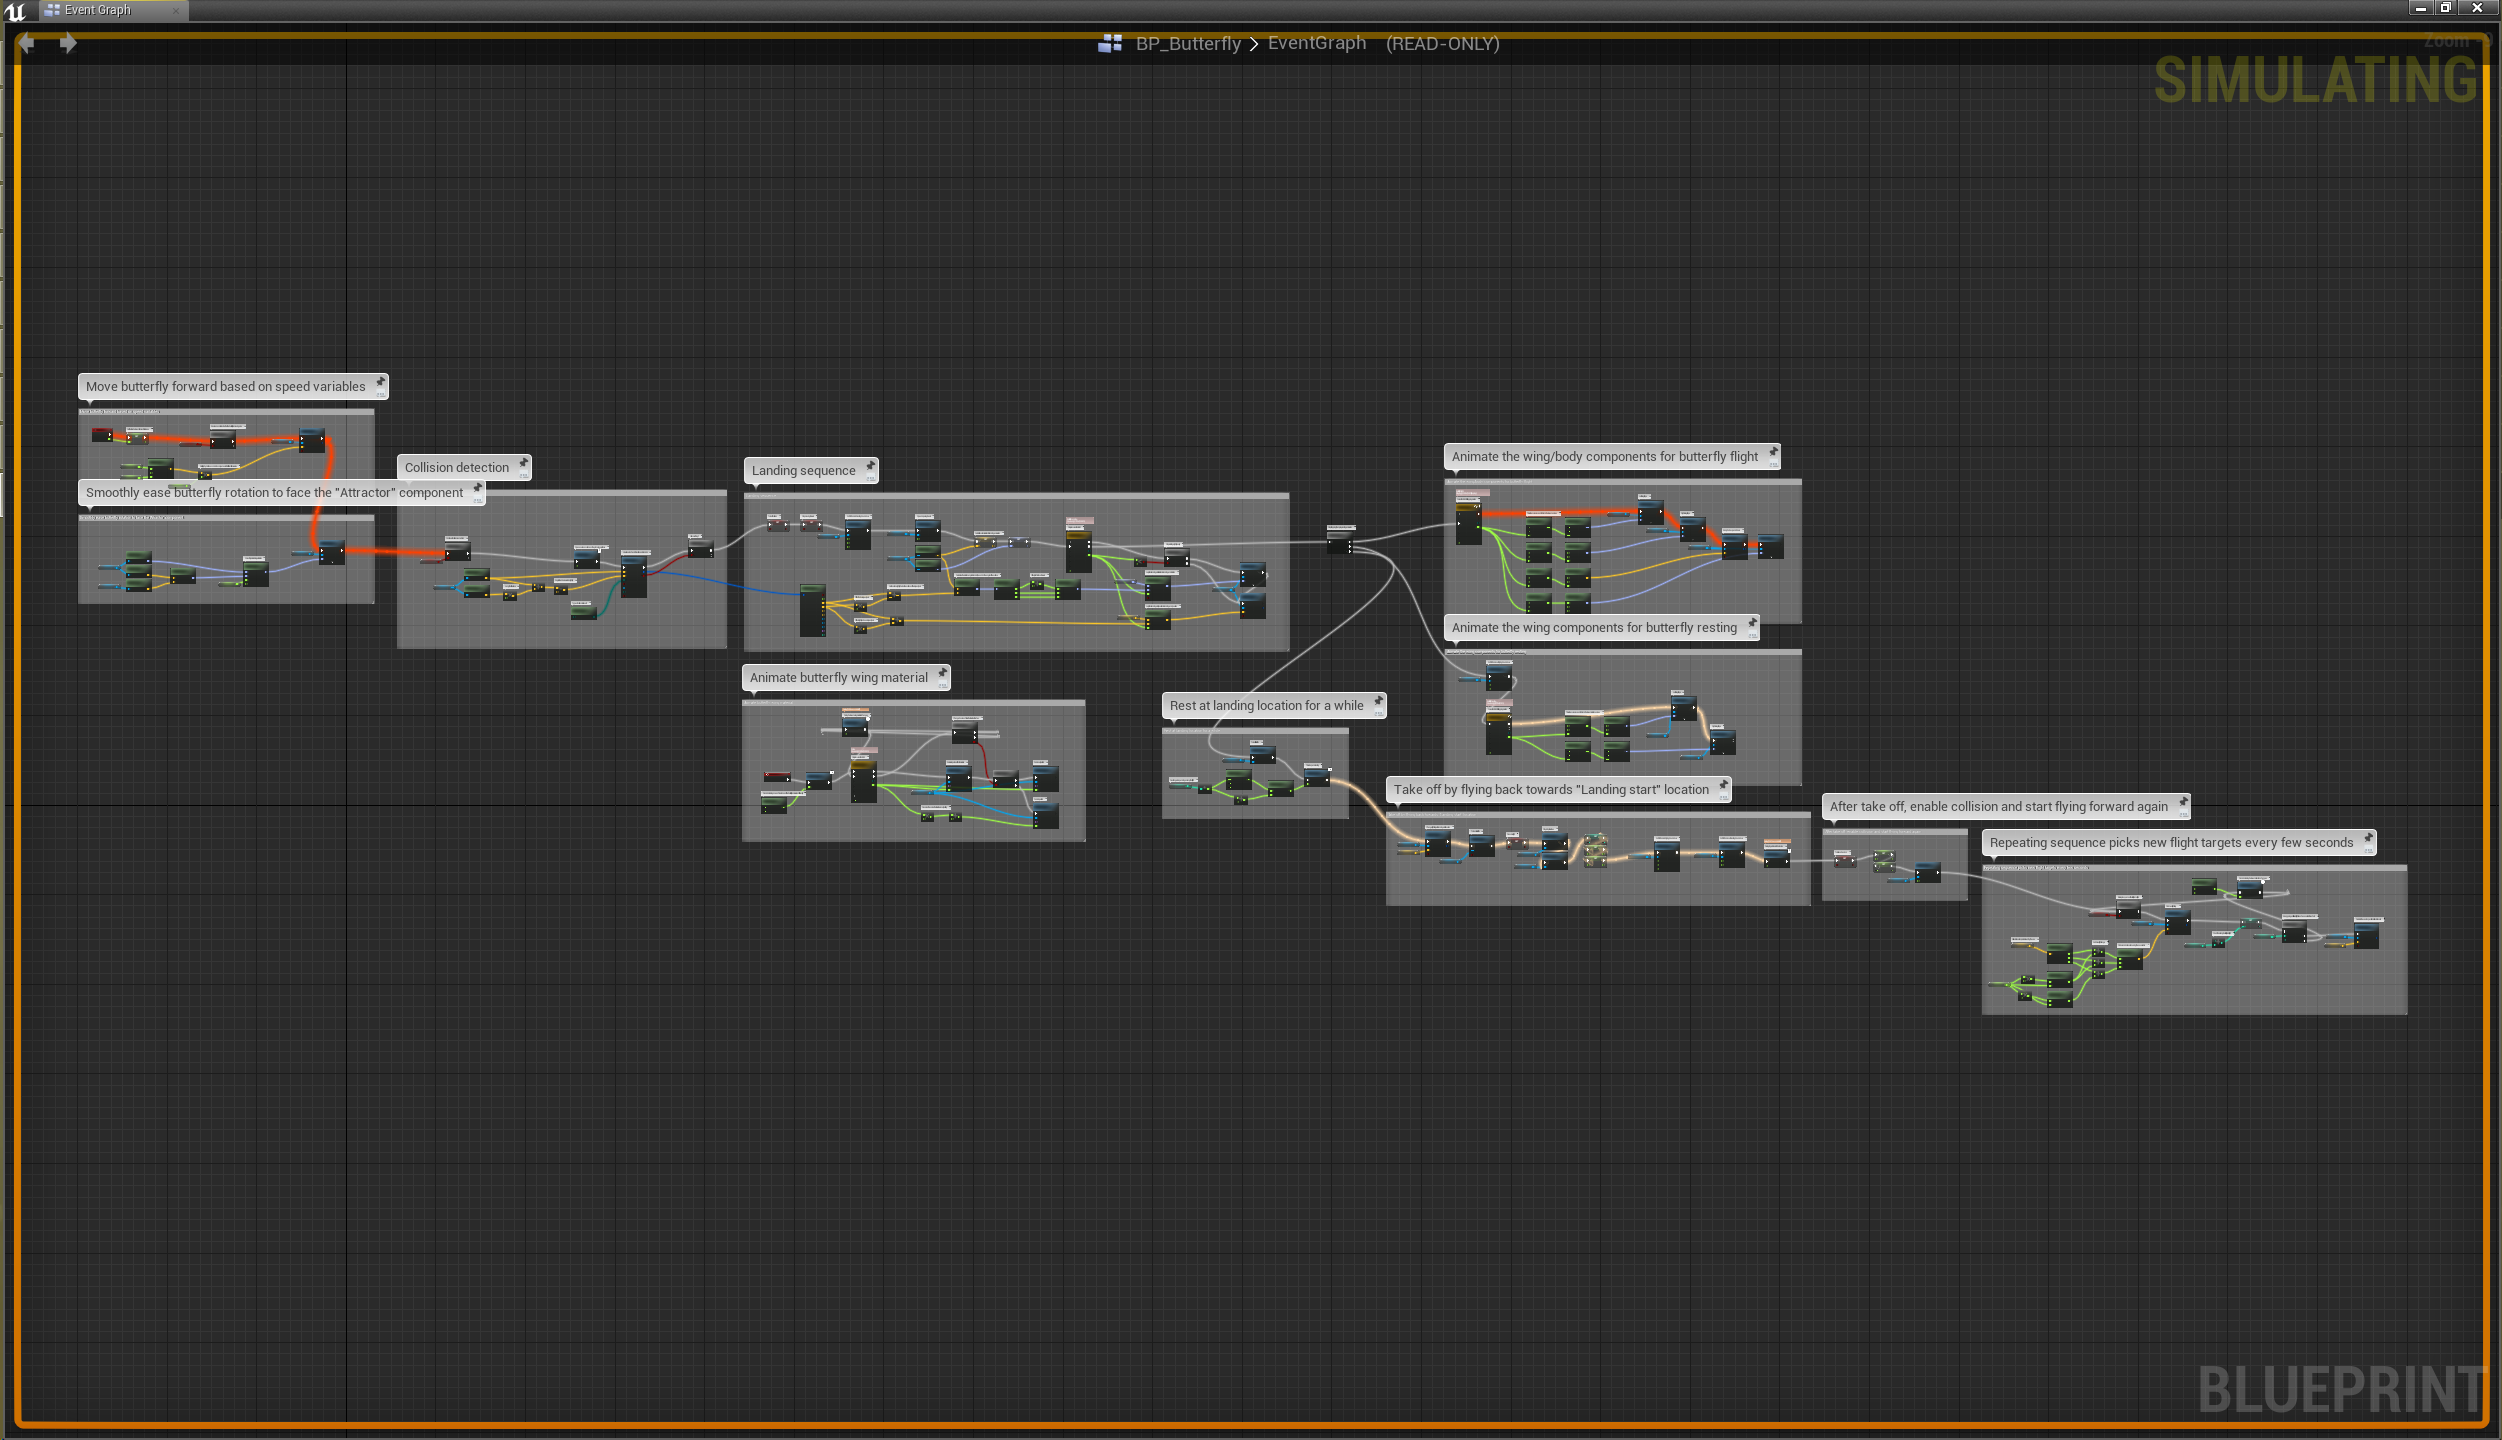
\includegraphics[width=\textwidth]{ue4-blueprint}
\caption{Unreal Engine 4 Blueprint Beispiel}
\end{figure}



\section{Grafik-Engines in Haskell}

\subsection{HGamer3D}

\textit{HGamer3D}\footnote{http://www.hgamer3d.org/} basiert auf (nich kompletten) Haskell-Bindings zu \textit{Ogre}\footnote{http://www.ogre3d.org/}. Ogre ist eine objektorientierte Open-Source Grafik-Engine geschrieben in C++. Ohne weiter auf die Fähigkeiten der Ogre Engine einzugehen, stellt sich oft die Adaptierunung von imperativen Bibliotheken auf funktionale Konzepte als aufwändig und nicht immer optimal heraus. Insbesondere das Erzeugen von Bindings zu komplexen \acsp{API}s ist immer noch eine hohe Hürde.

Auch wenn Ogre als Framework viele Strukturen und Lösungsansätze für gängige Probleme in der 3D Computergrafik und Spieleprogrammierung bereitstellt, ließen sich viele Ansätze auch direkt funktional umsetzen, ohne große und schwerfällige \acsp{API}s zähmen zu müssen.

Zum Beispiel verfolgen beide Welten zum Teil gänzlich andere Grundprinzipien. So sind Daten in Haskell prinzipiell unveränderlich während in C++ Daten prinzipiell veränderlich sind. Haskell erlaubt unter anderem deswegen andere Ansätze der Nebenläufigkeit (Concurrency). Speziell Nebenläufigkeiten stellen immer noch in komplexen Softwareprojekten eine große Hürde dar. Die Adaption einer C++-Biblithek kann das Ausnutzen vieler Vorteile von Haskell behindern (weitere Ausführungen in \fref{sec:warum-haskell}).

Zusätzlich entstehen durch Bindings zu externen Biblitheken neue Abhängigkeiten, die oft eine Anpassung der Tool-Chain erfordern, da sie nicht in das bestehende Ökosystem passen. Dies erhöht die Komplexität des Gesamtsystems. Die Erfahrung des Autos hat gezeigt, dass eigentlich jedes externes Binding früher oder später zu Komplikationen führt, spätestens dann, wenn die Anwendung die Entwicklungsumgebung verlässt. Doch lässt sich nicht jede Abhhängigkeit zu anderen Sprachen vermeiden. Insbesondere in der Grafikprogrammierung mit OpenGL werden die eigentlichen Bindings zu der OpenGL-API benötigt. Zusätzlich muss noch ein platformabhängiger Render-Kontext erzeugt werden.

Meinung des Autors: Es sollten möglichst wenige Fremdabhängigkeiten aus anderen Sprachen genutzt werden, leider ist dies nicht immer möglich (Weitere Ausführungen in \fref{sec:probleme-haskell}). Mit den Ogre Bindings wird die eine komplexe schwer funktional bezwingbare \acs{API} (z.B. OpenGL) mit einer anderen ersetzt.

\subsection{LambdaCube 3D}

\textit{LambdaCube 3D}\footnote{https://lambdacube3d.wordpress.com/} ist eine in Haskell definierte und beeindruckende \ac{DSL}, die es erlaubt Grafikanwendungen bis hin zum Shader komplett in Haskell zu formulieren. Da OpenGL eine komplexe und übersichtliche \acs{API} ist, ist die \ac{DSL} entsprechend komplex und unübersichtlich. Zusätzlich basiert das OpenGL Backend noch auf der Version 3.2. Die Dokumentation beschränkt sich auf den Blog und eine handvoll Beispielen, so dass es schwer ist einen Zugang zu der DSL zu erhalten.

Aber generell stellt sich die bei OpenGL die Frage, wie sinnvoll es ist die komplexe \acs{API} in einer anderen Sprache komplett abzubilden, mit all ihren erlaubten und nicht erlaubten Zuständen, die zusätzlich noch treiberspezifisch sind. Hinzu kommen diverse Erweiterungen, die oft Verhaltensweisen der \acs{API} massiv beeinflussen.

Die persönliche Einschätzung des Autors ist, dass sich OpenGL nicht in einem vertretbaren Aufwand komplett abbilden lässt. Der Aufwand wäre ungefähr mit dem vergleichbar, den Grafikkartenhersteller bei der Implementierung ihrer Grafikkartentreiber betreiben (weitere Ausführungen in \fref{chap:modern-opengl}). Deswegen sollte eine Auswahl der direkten OpenGL Bindings getroffen werden um sie punktuell in funktionale Konzepte zu gießen.

% \subsection{Elm}

% \subsection{Gloss}
% Gloss (2d) ist ein schönes Beispiel dafür wie sich mit einem OpenGL backend und mit der konzentration auf das wesentliche eine klare funktionale api schaffen lässt die einfach anzuwenden ist.


%%%%%%%%%%%%%%%%%%%%%%%%%%%%%% Überblick Modern OpenGL (4.0+)
\chapter{Überblick über Modern OpenGL}
\label{chap:modern-opengl}

\section{Von Fixed Pipeline zu Shadern}
Mit der Abkehr von der Fixed Pipeline begann die Ära von Modern OpenGL. Seit dem ist es möglich mit eigenen Shader-Programmen, in OpenGL meist geschrieben in GLSL, die einzelnen Stufen der Renderpipline anzupassen. Anfangs beschränkten sich die Stufen auf den Vertex sowie Fragment Shader. Im Laufe der Zeit sind jedoch eine Vielzahl von weiteren programmierbaren Shader-Stufen hinzu gekommen.

\begin{wrapfigure}{r}{0.5\linewidth}
\begin{centering}
	
\includegraphics[width=.5\textwidth]{OpenGL_Nov14}
\end{centering}
\end{wrapfigure}

Die Abkehr von der Fixed Pipeline erlaubte völlig neue Konzepte im Echtzeit-Rendering, anfangen von eigenen, anstatt fest vorgegeben, Beleuchtungsmodellen (siehe \fref{chap:pbr}) hin zu ausschließlich Fragment Shader basierten Grafikdemos\footnote{https://www.shadertoy.com/view/Xtf3Rn} sowie gänzlich neuen Echzeit-Rendering Konzepten\footnote{http://iquilezles.org/www/articles/raymarchingdf/raymarchingdf.htm}.

Während ursprünglich der Szene-Graph fest von OpenGL vorgegeben war und Vertices mindestens einmal jeweils und \textit{einzeln} von der CPU auf die GPU geladen werden mussten, änderte sich auch dies fundamental. Mit dem Ende der Fixed Pipeline wurden auch Buffer-Objekte immer wichtiger, so dass sich ganze Speicherbereiche direkt befüllen oder manipuliert ließen. Der Overhead, Vertices zur Grafikkarte zu schicken, reduzierte sich entsprechend deutlich. Inzwischen gibt es eine Vielzahl von unterschiedlichen Buffer-Typen für unterschiedliche Zwecke, die es sogar erlauben vollständig von Compute Shadern befüllt werden zu können.

Schließlich konnte der bis dato wesentliche Flaschenhals und limitierende Faktor, der Bus zur Grafikkarte, optimal genutzt werden, und war oft nur noch in initialen oder sporadischen Befüllungsvorgängen limitierend. Wie so oft tat sich entsprechend ein neuer Engpass auf. Dieser lag nun, und liegt oft noch immer, in der Implementierung der API, dem Treiber.

\section{Treiber Overhead \& Flexibilität}
\label{sec:overhead-und-flexibilitaet}

Dabei ist die OpenGL API und ihre Treiberimplementierung nicht per se ein Flaschenhals, doch erlaubt die gewachsene und rückwärtskompatibel gehaltene API unterschiedliche Pfade zum annähernd gleichen Ziel. Einige ältere Pfade bringen oft mehr Overhead mit sich, neuere erlauben die effektive Reduzierung der API Aufrufe (siehe \fref{fig:opengl-pfade}). \warn{erhöhung Flexibilität erwähnen} Die \ac{AZDO} Initiative von AMD, nVidia und Intel versucht seit ein bis zwei Jahren die schnelleren Pfade bei den Entwicklern bekannter zu machen. In einem knappen Überblick im folgenden dargestellt und in \fref{chap:haskell-modern-gl} auf ein mögliches Zusammenspiel mit Haskell genauer analysiert.

\begin{figure}
	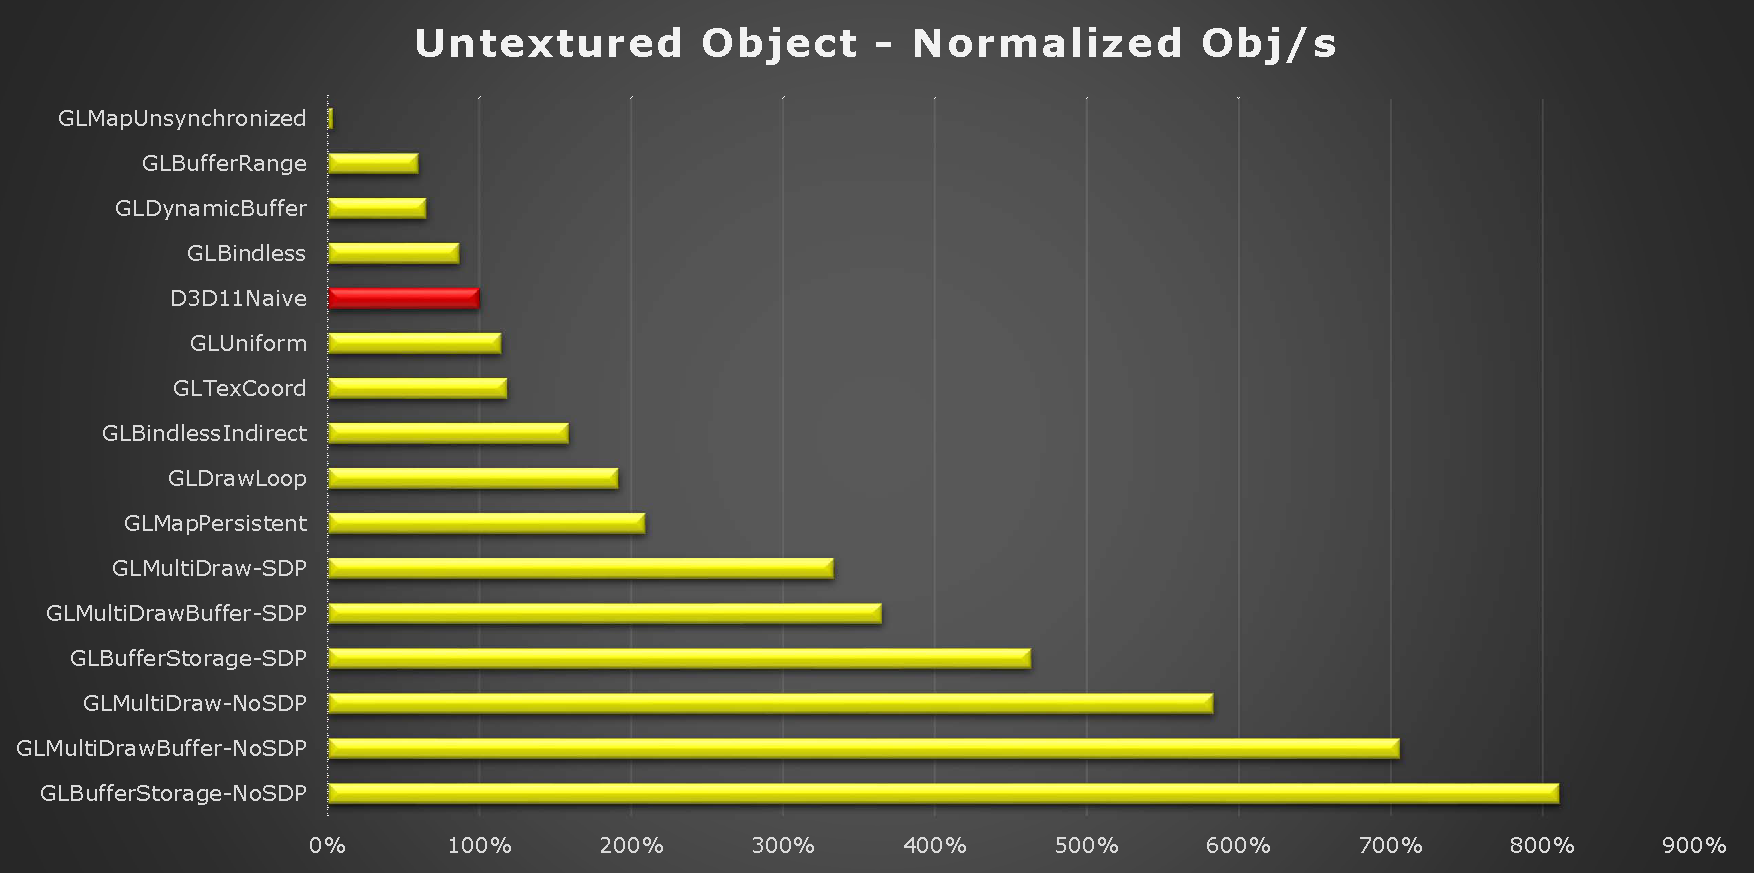
\includegraphics[width=\textwidth]{opengl-spread}
	\caption[Unterschiede in den OpenGL Renderpfaden]{Unterschiede in den OpenGL Renderpfaden \parencite[Seite 98]{Everitt2014}}
	\label{fig:opengl-pfade}
\end{figure}

\paragraph{\acl{MDI}} 
\ac{MDI} beschreibt das Ausführen von mehreren Draw-Calls mit einen API Aufruf. Anstatt für jedes Objekt die notwendigen Aufrufparameter des Draw-Calls separat anzugeben, werden die für alle Objekte notwendigen Parameter in einem OpenGL Buffer (\textit{Command Buffer}) zusammengefasst. Der einzelne indirekte Draw-Call entspricht im wesentlichen nur noch einem Aufruf mit einem Zeiger auf den Inhalt des Command Buffers. Die Parameter können entweder von der CPU aus bestimmt werden oder direkt auf der GPU (z.B. durch View-Frustum Culling auf der GPU). Das Konzept des indirekten Renderns fasst das indexbasierte Rendern und instanziiertes Rendern zusammen\footnote{https://www.opengl.org/wiki/Vertex\_Rendering\#Indirect\_rendering}. Der Command-Buffer in Verbindung mit dem Draw-Call beschreibt ausschließlich die Gestalt des für allen Objekte gemeinsamen \textit{Vertex}-Buffers. Da nun für jedes Objekt kein seperater Draw-Call ausgeführt wird, können auch keine individuellen Daten per Object (zum Beispiel Transformationsmatrizen) an die Shader übergeben werden. Das macht es erforderlich entsprechende Daten gebündelt in einem Array oder \ac{SSBO} dem Shader zu übergeben. Der indizierte Zugriff kann im Shader dann über eingebaute Variablen erfolgen. Dies reduziert zusätzlich den Overhead.

\paragraph{\acl{DSA}} Ein weiterer Schritt zur Reduzierung des Treiber Overheads ist die \ac{DSA} Erweiterung von OpenGL \parencite{Killgard2014} die in den nächsten Jahren mit OpenGL 4.5 Einzug halten wird. Die unterschiedlichen OpenGL Objekte besitzen meistens einen eigenen internen Zustand. Soll dieser Zustand aktualisiert oder abgefragt werden, müssen die Objekte zuvor über Selektoren gebunden werden. Dies ist oft nicht nur fehleranfällig sondern sorgt für wenig intuitiven und lärmenden Quelltext. Zusätzlich erhöht es den API Overhead. 

Mit \ac{DSA} fällt das Selektieren von Objekten vor dem Zugriff auf den Zustand weg und es werden neue Operationen bereit gestellt, die das entsprechende OpenGL Objekt als Parameter erwarten. So lässt sich der Zustand abfragen und manipulieren ohne dass das Objekt vorher im globalen Zustand gebunden werden muss. Dies reduziert den Overhead etwas. Im wesentlichen vereinfacht es die Programmierung mit OpenGL Objekten und erlaubt die Kapselung von Funktionalitäten und erleichtert damit die Umsetzung von komponierbaren Bibliotheken \fref{chap:haskell-modern-gl}.

\paragraph{Separate Program Objects} Auch wenn \ac{DSA} erst mit OpenGL 4.5 breiten Einzug ins \textit{Core} Profil genommen hat, fand die Erweiterung |ARB_separate_program_objects| \parencite{Killgard2011} schon mit Version 4.1 ihren Weg in das \textit{Core} Profil. Zuvor mussten die unterschiedlichen Shader Stufen (Vertex, Geoemetry, Fragment usw.) in ein monolithisches Programm übersetzt werden. Mit der Erweiterung können die einzelnen Stufen unabhängig von einander übersetzt werden. Die Program-Objekte lassen sich dann, unter der Berücksichtungen der Schnittstellen, frei zu einer Programm-Pipeline zusammen setzen. Zusätzlich führt die Erweiterung \ac{DSA} für die Program-Objekte ein, so dass nicht mehr vor der Uniform-Variablenzuwesung die Shader-Objekte gebunden werden müssen. Stattdessen können die Zuweisungen direkt mit dem Program-Objekt durchgeführt werden \warn{link section: \fref{chap:haskell-modern-gl}}.

% ### http://www.g-truc.net/post-0320.html

\section{Vulkan}

\textit{Vulkan} (vormals \textit{glNext}) und \textit{SPIR-V} ist der nächste Schritt (oder Versuch) der \textit{Khronos Group} sich der über Jahrzente gesammelten Altlasten der OpenGL-API zu entledigen. Vulkan wurde im März 2015 als frischer Neustart der Grafik-API angekündigt. Noch ist die Spezifikation am entstehen, aber das erklärte Ziel von Vulkan ist die Reduzierung des CPU Overheads, die breitere Ermöglichung von Multi-Threading und die Abschaffung des impliziten OpenGL Context hin zu einer expliziten API. Neben \textit{Vulkan} wurde \textit{SPIR-V} als eine neue Shader \ac{IL} bzw. Zwischensprache vorgestellt. SPIR-V soll neue Freiräume schaffen eigene Shader-Sprachen sowie Analsyse- und Debuggingtools zu entwickeln\parencite{Olson2015}.

Die Gründe für einen harten Schnitt in der API sind auf zwei Seiten zu suchen. Zum einen ist für den API-Anwender die OpenGL-API wie bereits erwähnt voller Fallstricke. Auf der anderen Seite sind die aktuellen OpenGL Treiber zu einem großen Flickenteppich verkommen. Viele Treiberimplementierungen sind voller Weichen und und Spezialfällen, um bekannte Fehler in der Anwendung der API abzufangen oder potenziell langsame Pfade in schnellere Pfade zu übersetzen \parencite{gamedevnet:glnext}.

\begin{figure*}
\centering
	
\includegraphics[height=2cm]{Vulkan_Mar15}
	
\includegraphics[height=2cm]{SPIR_Nov14}
\end{figure*}




%%%%%%%%%%%%%%%%%%%%%%%%%%%%%% Loesungen durch Haskell
% \chapter{Lösungsansätze durch Funktionale Programmierung}\label{chap:loesungen-durch-fp}

\epigraph{"`In our profession, we desperately need all the help we can get. If a clean shop floor reduces accidents, and well-organized shop tools increase productivity, then I’m all for them."'}{James O. Coplien, aus dem Vorwort zu \spacedlowsmallcaps{Clean Code: A Handbook of Agile Software Craftsmanship}}

Wie schon in \fref{chap:engine-uebersicht} beschrieben, sind Spiele- und Grafik-Engines äußerst komplexe Softwareprojekte. Auch wenn Haskell oft als reine akademische Sprache angesehen wird, findet Haskell inzwischen praktische Anwendung in unterschiedlichen Bereichen. Haskell besitzt dabei einige Vorzüge, die viele andere Sprachen nicht bieten oder nur unter großem Aufwand bieten können.

\section{Statische Typisierung}\label{sec:statische-typisierung}

Die statische Typisierung elimiert eine ganze Kategorie von Fehlerquellen, die sich  in untypisierten oder dynamisch typisierten Sprachen zeigen. Die statische Typisierung und das Fehlen von implizieten Seiteneffekten sorgt für eindeutige und klare Signaturen. Auch wenn in der Praxis nicht jede Funktion formal auf ihre Korrektheit bewiesen werden kann, erleichtern die klaren Signaturen und die statischen Typen die Ad-hoc Beweisführung (Reasoning), die jeder Entwickler automatisch im Kopf beim Lesen oder Schreiben von Programmen mitführt. Viele Implementierungen von Funktionen ergeben sich oft schon aus der Signatur.

Haskell eliminiert durch das Typ-System viele gängige Fehlerquellen in Software. \texttt{NULL} Referenzen werden vom Erfinder Tony Hoare rückblickend selber als "`[...] my billion-dollar mistake"' bezeichnet\footnote{http://www.infoq.com/presentations/Null-References-The-Billion-Dollar-Mistake-Tony-Hoare}. Sie bilden immer noch eine der größten Fehlerqullen in Software, wenn die Sprache implizte \texttt{NULL} Referenzen erlaubt. 

\begin{quote}
"`Static analysis helps, but NULL problems remain the top fault in our codebase."'\footnote{\label{note:carmack-null}https://twitter.com/id\_aa\_carmack/status/325019679720615936}
\end{quote}

Durch die explizite Kennzeichnung von optionalen Werten durch |Maybe| schließt Haskell kategorisch eine der größten Fehlerquellen in Softwareprojekten noch zum Übersetzungszeitpunkt aus. Generell gilt, dass Fehler, die schon zur Übersetzungszeit auftreten, einen geringeren kritischen Einfluss auf das Entwicklungs- bzw. Produktionssystem haben als Laufzeitfehler. Es ist trivial zu verhindern, dass Kompilierungsfehler überhaupt schon in das Entwicklungssystem gelangen\footnote{Beispielsweise durch ein \textit{Continious Integration} System}. Dahingegend ist es keine Seltenheit, dass Laufzeitfehler den Entwicklunszyklus lange genug unentdeckt überstehen, bis sie in das Produktionssystem gelangen. Das ist ein starkes Argument für die Philosophie, möglichst viele Fehlerquellen zum Kompilierungszeitpunkt auszuschließen.

\section{Haskell als Kommunikationsmittel}

Haskell gilt als eine sehr ausdrucksstarke Programmiersprache. Viele funktionale Konzepte erlauben einen neuen und oft höheren Abstraktionsgrad, als zum Beispiel rein Objekt orientierten Sprachen. Funktionale Programmierung erzwingt und begünstigt die Zerlegung von Problemen in kleine Teilprobleme. Kleine Teilprobleme sind einfacher zu verstehen und leichter zu warten. Die klaren ausdrucksstarken Signaturen bilden eine solide Basis für die Kommunikation zwischen den Entwicklern über den Programmcode. 

\section{Komposition}

Die genannten wesentlichen Eigenschaften erlauben in Kombination das Schreiben von wiederverwendbaren und komponierbaren Funktionen.Der Grad der Komponierbarkeit von Systembestandteilen ist eine nicht direkt messbare Größe und lässt sich nicht formal definieren. Intuitiv gilt ein System und seine Bestandteile als gut komponierbar, wenn sich die Bestandteile ohne großen Aufwand frei kombinieren lassen. Durch die Kombination von gut komponierbaren Elementen sollte die Komplexität des Kombinats nicht übermäßig ansteigen. Im Ideal entspricht die Komplexität des Kombinats der Summe der Komplexitäten der Teilkomponenten \parencite[Seite 19]{Blackheath2013}.

Kleine übersichtliche und gut komponierbare Elemente führen zu verständlicheren, zugänglicheren und wartbaren Gesamtsystemen \parencite[Seite 12 ff.]{Stewart2015}. Dies zeigt sich dadurch, dass bereits viele kleine spezialisierte Projekte in Haskell entwickelt wurden, die sich leicht zu einem größeren Projekt zusammensetzen lassen. Die referenzielle Transparenz und das Fehlen von impliziten Seiteneffekten spielen hierbei eine wesentliche Rolle. Zusätzlich ist die Verständigung über klare funktionale bzw. mathematische Konzepte und Regeln eindeutig. Ein |Functor| bleibt ein |Functor| und die Anwendung eines |Functor|s ist überall verständlich. Diese Konzepte erhöhen die Kompositionsfähigkeit und Wiederverwendbarkeit der entwickelten Elemente.

\section{Nebenläufigkeiten}
\label{sec:nebenlaeufigkeiten}

Tim Sweeny von \textit{Epic Games} nennt das "`Shared State Concurrency"' Model aus C++, Java oder C\# eine "`Huge productivity burden"' und weiter sagt er: "`Purely Functional is the right default"'\footnote{\cite[Vgl.][Seite 42 u. Seite 56]{Sweeney2006}\label{note:sweeney-mainstream}}. John Carmack, Gründer von \textit{id Software} und nun CTO bei \textit{Oculus VR}: "`[...] banning mutable shared state. Easier said than done, of course."'\footref{note:carmack-null}.

Die Veränderlichkeit von Daten (mutable) stellt ein großes Hindernis für elegante Nebenläufigkeit in den genannten Sprachen dar. Hinzu kommt, dass Funktionen bzw. Methoden in den genannten Sprachen keine Garantie geben können, dass sie auf ihren Daten garantiert seiteneffektsfrei arbeiten. Das macht es aufwändig Nebenläufige System zu entwickeln, da Nebenläufigkeit mit einem großen Synchronisierungs- und Verwaltungsaufwand verbunden ist.

\begin{quote}
"`In a concurrent world, imperative is the wrong default!"'\footref{note:sweeney-mainstream}
\end{quote}

% Neben den grundsätzlichen Gegebenheiten für elegante Nebenläufigkeit in Haskell, bietet Haskell STM


%%%%%%%%%%%%%%%%%%%%%%%%%%%%%% Funktionale Progammierung & Modern GL
\chapter{Funktionale Programmierung \& Modern OpenGL}
\label{chap:haskell-modern-gl}

\begingroup
% \setlength\intextsep{0pt}
\section{Anwendung von Haskell mit Modern OpenGL Konzepten}\label{sec:haskell-gl-anwendung}

Die in \fref{sec:overhead-und-flexibilitaet} genannten Erweiterungen wurden entweder mit dem Ziel entwickelt die \textit{OpenGL} \ac{API} zu vereinfachen oder den \ac{API} Overhead zu reduzieren. Wie diese neuen Konzepte mit Haskell harmonieren wird im folgenden beschrieben.

\paragraph{Direct State Access \& Separate Program Objects} Die Verwendung von Buffern für Daten und Kommandos (\ac{MDI}) und der dadurch reduzierte API Overhead soll neue Spielräume für die CPU eröffnen. Dies wird oft damit beworben, dass die CPU wieder "`interessantere"' Aufgaben übernehmen kann, ansatt Zeit mit dem Aufrufen der Grafik-\ac{API} zu verschwenden. Die neuen Spielräumen können aber auch dazu genutzten werden, neue Ansätze zur Produktivitätssteigung zu wählen. Die generelle Reduzierung des Overheads kommt dabei auch Haskell zugute.

\begin{wrapfigure}{r}{0.5\linewidth}
\centering
\fbox{
\begin{minipage}[t]{0.9\linewidth}
\begin{smaller}
\paragraph{Quine}
Quine\footnote{https://github.com/ekmett/quine/} ist ein kleines Hobby Projekt von Edward Kmett. Aktuell basiert das Projekt auf den neuen \textit{OpenGL} Haskell-Bindings der \texttt{gl} Bibliothek. Die Demo Szenen sind aktuell nur Fragment-Shader Demos von Shadertoy\footnote{https://www.shadertoy.com/}. Langfristiges Ziel von Quine ist laut Edward Kmett eine Bibliothek in Haskell zu erschaffen die eine Sammlung der Best-Practices von Modern OpenGL zugänglich macht. Der Autor dieser Arbeit beteiligt sich an dem Projekt und hat schon kleinere allgemeine Teile aus dem hier beschriebenen Projekt nach Quine portiert.
\end{smaller}
\end{minipage}
}
\end{wrapfigure}

Zusätzlich lässt sich Haskell dazu als Hebel nutzen, die bessere Modularität von \ac{DSA} besser auszuschöpfen. Die \textit{Separate Program Objects} lassen sich dabei schon in \textit{OpenGL} 4.1 als Vorboten von \ac{DSA} betrachten. Wie bereits beschrieben lassen sich über diese \textit{OpenGL} Erweiterung die Uniform Variablen der einzelnen Shader-Stufen direkt über das Program-Objekt setzen. In Verbindung mit einer |StateVar| (siehe Beispielimplementierung \fref{sec:src-statevar}) und wenigen zusätzlichen Definitionen, lassen sich in Haskell elegante Schnittstellendatentypen für Shader definieren, die sich in Zukunft automatisch generieren ließen. \ref{lst:uniform-beispiel} gibt ein Beispiel, wie sich eine Shader-Schnittstelle über funktionale Konzepte zusammensetzen lässt. Ein relevanter Auszug findet sich in \fref{lst:uniform-beispiel-auszug}:

\haskellcode[caption={Shader-Schnittstelle (Auszug)},label={lst:uniform-beispiel-auszug},firstline=67]{src/uniform-beispiel.hs}
\endgroup

Der Beispielcode zeigt, wie die Funktion |fragmentInterface| mit Hilfe der |Applicative| Implementierung der |UniformVar| das Shader Interface modular zusammensetzt. Das werden einzelne Bausteine wie |materialUniform| und |intUniform| komponiert. Details zur |Applicative| Klasse in Haskell finden sich im nächsten \fref{chap:ueberblick-pipeline}. Die Basisbausteine für die GLSL Uniform Basistypen wurden beispielsweise bereits in Quine (siehe Kasten) implementiert.


\paragraph{Vulkan} Mit \textit{Vulkan} sollen neue Möglichkeiten geschaffen werden, die Buffer in Multi-Threading Systemen zu verwenden. Haskell besitzt herausragende Multi-Threading Eigenschaften, wie in \fref{sec:nebenlaeufigkeiten} umrissen wurde. In vielen imperativen Sprachen stellt Multi-Threading immer noch eine besondere Herausforderung dar (siehe \fref{sec:nebenlaeufigkeiten}). Viele Engines verwenden deswegen Multi-Threading nur zögerlich und äußerst vorsichtig \parencite[Seite 42]{Sweeney2006}. Haskell zeigt, dass viele Grundprinzipien für Nebenläufigkeiten die erste Wahl sind. Konzepte wie |MVar|s oder \ac{STM} könnten das Synchronisieren von Buffer-Objekte über mehrere Threads hinweg vereinfachen \parencite{Marlow2012}.

\section{Grafik-Engines in Haskell}

C bzw. C++ ist der Industriestandard in der Grafik- und Spieleprogrammierung. Alle kommerziell relevanten Spieleengines sind in C++ entwickelt, unter ihnen: \textit{CryEngine}, \textit{Unreal Engine 4}\footnote{\cite{EpicGames2014}} oder \textit{idTech 5}\footnote{idTech 4 wechselte auf C++, idTech 5 basiert auf idTech 4 \parencite{IdSoftware2011}}. Doch gibt es auch Open-Source Engines die in anderen Sprachen implementiert wurden. Die folgende Betrachtung beschränkt sich auf jene Engines, die entweder direkt in Haskell umgesetzt wurden oder deren Bindings auf bestehende Open-Source Engines aus anderen Sprachen basieren. Zusätzlich gibt der Autor zu jedem Projekt eine subjektive Einschätzung über die Probleme der gewählten Lösungen und warum der Autor der Meinung ist, dass eine möglichst rein funktionale Lösung entwickelt werden sollte. Letzter Punkt wird in \fref{chap:resultat} noch genauer ausgeführt.

\subsection{HGamer3D}

\textit{HGamer3D}\footnote{http://www.hgamer3d.org/} basiert auf (nicht vollständigen) Haskell-Bindings zu \textit{Ogre}\footnote{http://www.ogre3d.org/}. \textit{Ogre} ist eine objektorientierte Open-Source Grafik-Engine geschrieben in C++. Ohne weiter auf die Fähigkeiten der Ogre Engine einzugehen, stellt sich oft die Adaptierunung von imperativen Bibliotheken auf funktionale Konzepte als aufwändig und nicht immer optimal heraus. Die Notwendigkeit Haskell-Bindings zu komplexen C++ \acsp{API} manuell erzeugen zu müssen setzt hohe Hürden.

Auch wenn \textit{Ogre} als Framework viele Strukturen und Lösungsansätze für gängige Probleme in der 3D Computergrafik und Spieleprogrammierung bereitstellt, ließen sich viele Ansätze auch direkt funktional umsetzen, ohne große und schwerfällige \acsp{API} adaptieren zu müssen. Die Adaption einer C++-Biblithek kann das Ausnutzen vieler Vorteile von Haskell behindern (z.B. Nebenläufigkeit, oder referenzielle Transparenz).

Zusätzlich entstehen durch Bindings zu externen Bibliotheken neue Abhängigkeiten, die oft eine Anpassung der Tool-Chain erfordern, da die Abhängigkeiten nicht in das bestehende Ökosystem passen. Dies erhöht die Komplexität des Gesamtsystems. Die Erfahrung des Autors hat gezeigt, dass externe Bindings oft zu Komplikationen führen, spätestens dann, wenn die Anwendung die Entwicklungsumgebung verlässt. In der Praxis lassen sich aber selten Abhhängigkeiten zu anderen Sprachen komplett vermeiden. Insbesondere in der Grafikprogrammierung mit \textit{OpenGL} werden die eigentlichen Bindings zu der \textit{OpenGL}-API benötigt. Zusätzlich muss ein plattformabhängiger Render-Kontext erzeugt werden. Dessen Erzeugung ist nicht Teil von \textit{OpenGL} und erfordert eine weitere sprachfremde Komponente.

\paragraph{Meinung des Autors} Es sollten möglichst wenige Fremdabhängigkeiten aus anderen Sprachen genutzt werden, leider ist dies nicht immer möglich (Weitere Ausführungen in \fref{sec:probleme-haskell}). Mit den \textit{Ogre} Bindings wird die eine komplexe schwer funktional bezwingbare \acs{API} (\textit{OpenGL}) mit einer anderen ersetzt. Vorteil ist unbestritten, dass die Engine ausgereift ist und vieles nicht erst neu implementiert werden muss.

\subsection{LambdaCube 3D}

\textit{LambdaCube 3D}\footnote{https://lambdacube3d.wordpress.com/} ist eine in Haskell definierte und mächtige \ac{DSL}, die es erlaubt Grafikanwendungen bis hin zum Shader komplett in Haskell zu formulieren. Da \textit{OpenGL} eine komplexe und unübersichtliche \acs{API} ist, ist die \ac{DSL} entsprechend komplex und unübersichtlich. Zusätzlich basiert das \textit{OpenGL}-Backend noch auf der Version 3.2, sodass viele neue Shader-Möglichkeiten (z.B. Compute Shader ab 4.3) gar nicht abgedeckt sind. Die Dokumentation beschränkt sich auf den Blog und eine handvoll Beispielen. Das erschwert das Erlernen der DSL deutlich.

Auch generell stellt sich bei \textit{OpenGL} die Frage, wie sinnvoll es ist die komplexe \acs{API} in einer anderen Sprache komplett abzubilden. \textit{OpenGL} besitzt viele erlaubte und nicht erlaubten Zustände. Die erlaubten und nicht erlaubten Zustände sind zudem mitunter treiberspezifisch. Hinzu kommen diverse Erweiterungen, die die Verhaltensweise der \acs{API} massiv beeinflussen und gültige und ungültige Zustände hinzufügen oder entfernen können (siehe \fref{sec:vulkan}).

\paragraph{Meinung des Autors} \textit{OpenGL} lässt sich nicht in einem vertretbaren Aufwand komplett abbilden. Der Aufwand wäre ungefähr mit dem vergleichbar, den Grafikkartenhersteller bei der Implementierung ihrer Grafikkartentreiber betreiben (weitere Ausführungen in \fref{sec:vulkan}). Deswegen sollte eine Auswahl der direkten \textit{OpenGL} Bindings getroffen werden um sie punktuell in funktionale Konzepte zu gießen.

% \subsection{Elm}

% \subsection{Gloss}
% Gloss (2d) ist ein schönes Beispiel dafür wie sich mit einem \textit{OpenGL} backend und mit der konzentration auf das wesentliche eine klare funktionale api schaffen lässt die einfach anzuwenden ist.


%%%%%%%%%%%%%%%%%%%%%%%%%%%%%% Entwicklung einer Grafikengine in Haskell
\chapter{Überblick über das Rendersystem der Engine}
\label{chap:ueberblick-pipeline}

Auf Grund des Umfangs des Projekts ist es nicht möglich einen all umfassenden Überblick über die Engine zu geben. Die Betrachtung im Detail beschränkt sich im Folgenden auf die entwickelte Renderkomponente der Engine und die dahinter stehenden Konzepte und Überlegungen. Es wird anhand der Quelltextbeispiele demonstriert, dass sich der Umfang der funktionalen Konzepte überschaubar gestaltet. Und dennoch ermöglichen diese Konzepte eine hohe Flexibilität. Sobald die Konzepte verstanden sind, erhöht die Kompaktheit dieser Konzepte die Lesbarkeit und erleichtert den Zugang zu strukturellen ähnlich gelagerten Problemen.

\section{Das Rendersystem}

% anforderung
Moderne Renderverfahren, wie zum Beispiel Deferred Rendering, bestehen aus mehreren einzelnen Renderschritten. In der Regel erzeugt jeder Renderschritt Daten, oft in Form von Texturen oder Buffern. Die Daten dienen den nachfolgenden Renderschritten als Basis für weitere Berechnungen. Daraus ergibt sich ein Abhängigkeitsnetzwerk aus Eingabe und Ausgaben einzelner Renderschritte. Ein Renderschritt kann wiederum aus kleineren Renderschritten zusammengesetzt sein.

Bei der Entwicklung der Renderkomponente wurde das Ziel verfolgt, dass sich die einzelen Renderschritte möglichst komponierbar anwenden lassen. Zusätzlich sollen die einzelen Renderschritte die Möglichkeit erhalten ihren inneren Zustand selbst zu verwalten und Implementierungsdetails zu verbergen. Auf Kompositionsebene sollen Implementierungsdetails möglichst vermeidbar sein.

Die Konzeption des Renderystems startet mit einer formal abstrakten Definition auf Basis eines Mealy Automatens. Die formale Definition wird mit weiteren abstrakten funktionalen Konzepten schrittweise erweitert. Kleine praxisnahe Beispiele demonstrieren, wie die Erweiterungen die Flexibilität und Komponierbarkeit der Renderschritte erhöhen.

\subsection{Mealy als formale Basis}

Das Rendersystem basiert auf dem Konzept eines Mealy Automatens \parencite{Mealy1955}. Ein Mealy Automat ist ein \acl{FST}, ein spezieller endlicher Automat, der nicht nur seine Eingabesprache vom Eingabeband akzeptiert, sondern auch eine Ausgabe auf einem Ausgabeband erzeugt. Ein Transduktor übersetzt die Eingabesprache in eine Ausgabesprache. Bei dem Mealy Automaten, als spezielle Form eines \ac{FST}, definiert sich die Ausgabe über den momentanen Zustand und die Eingabe auf diesem Zustand. Formal lässt sich ein Mealy Automat $\mathbfcal{M}$ als 6-Tupel wie folgt definieren:

\begin{definition}
\begin{align}
\mathbfcal{M} = \left( Q, \Sigma, \Omega, \delta, \lambda, q_0 \right)
\label{def:mealy-formal}
\end{align}
\begin{align*}
	\text{mit}\\
	Q &: \text{Endliche Menge von Zuständen} \\
	\Sigma  &:\text{Endliches Eingabealphabet} \\
	\Omega  &:\text{Endliches Ausgabealphabet} \\
	\delta  &:\text{Zustandsübergangsfunktion}\ Q \times \Sigma \rightarrow Q \\
	\lambda &:\text{Ausgabefunktion}\ Q \times \Sigma \rightarrow \Omega \\
	q_0 &: \text{Startzustand}
\end{align*}
\end{definition}

Die Definition ließe sich noch um die Menge der finalen Endzustände $F \subseteq Q$ hin zu einem 7-Tupel erweitern. In unserem Konzept verzichten wir auf definierte Endzustände, da wir prinzipiell jede Eingabe akzeptieren. Nicht akzpetierbare Eingaben stellen wir als externe Ausnahmefälle (Exceptions) dar. Ein vereinfachtes Beispiel für eine nicht akzeptierbare Eingabe ist die Eingabe $\bot$, nach der unser gesamtes System in einen undefinierten Zustand $\bot$ wechselt.

\paragraph{Abstrakte Definition in Haskell}
\label{sec:abstrakte-definition-haskell}

Ein Mealy Automat lässt sich in Haskell abstrakt wie in \fref{lst:haskell-mealy} definieren. {\ttfamily a} beschreibt die Eingabe als Äquivalent zum Eingabealphabet $\Sigma$ der formalen Definition und analog beschreibt |b| die Ausgabe als Äquivalent zum Ausgabealphabet $\Omega$. Die Zustandsübergangsfunktion $\delta$ und die Ausgabefunktion $\lambda$ ergibt sich aus der jeweils konkreten Implementierung des Mealy. Die Menge der Zustände $Q$ wird jeweils von der konkreten Mealy Implementierung gekapselt, wie in \fref{lst:state-mealy-beispiel} anhand eines Beispiels veranschaulicht wird.

Im Gegensatz zur formalen Definition eines Mealy Automatens lässt sich feststellen, dass die in Haskell gewählte Form des Mealy Automatens weit mehr als nur ein endlicher Automat ist. Die Mächtigkeit des Ein- und Ausgabealphabets ist in der Haskell-Definition nicht beschränkt. Beispielsweise lässt sich ein Haskell-Mealy Automat als Zählmaschine umsetzen. Die Maschine akzeptiert die Menge der natürlichen Zahlen (abzählbar unendlich) und zählt zum Beispiel die geraden Zahlen. Daraus folgt, dass bei dem Haskell-Mealy Automaten die Menge der Zustände unendlich sein kann.

\begin{haskell}[label={lst:haskell-mealy},caption={[Definition Mealy in Haskell]Definition Mealy in Haskell\protect\footnotemark}]
newtype Mealy a b = Mealy { runMealy :: a -> (b, Mealy a b) }
\end{haskell}
\footnotetext{https://hackage.haskell.org/package/machines-0.4.1/docs/Data-Machine-Mealy.html}

Für diese Definition einer Meleay existieren einige nützliche Klassen. Die Klassen werden an dieser Stelle übersprungen, da 
später für die erweiterte monadische Definition eigene Implementierungen entwickelt werden (\fref{sec:konkret-rendersystem}).

Allgemein lässt sich die Funktionsweise von |Mealy| wie folgt beschreiben:\\
|runMealy| führt mit einer Eingabe vom Typ |a| den |Mealy| aus und erzeugt eine Ausgabe vom Typ |b| und einen neuen Mealy-Automaten, der die selbe Eingabesprache in die selbe Ausgabesprache übersetzt. Im einfachsten Fall ist der neu erzeugte Mealy Automat exakt der gleiche aus dem vorherigen Schritt. Ist dies für das gesamte Eingabealphabet gegeben, gilt der Automat als zustandslos.

Für die Konstruktion eines Mealy Automaten mit lokalem Zustand folgt aus der formalen Definition \ref{def:mealy-formal} die Notwendigkeit einer Zustandsübergangsfunktion $\delta$ und einem Startzustand $q_0$. Hiefür definieren wir uns in \fref{lst:state-mealy-ctr} die Hilfsfunktion |localStateMealy|. Der erste Parameter |s -> a -> (b, s)| beschreibt die Kombination der beiden Funktionen $\delta$ und $\lambda$, der zweite Parameter den Startzustand $q_0$.

\begin{haskell}[label={lst:state-mealy-ctr},caption={[Konstruktion Mealy mit lokalem Zustand]Hilfsfunktion zur Konstruktion eines Mealy-Automatens mit lokalem Zustand}]
localStateMealy :: (s -> a -> (b, s)) -> s -> Mealy a b
localStateMealy stateTransition initState = run initState where
  run state = Mealy (\input -> 
    let (output, state') = stateTransition state input 
    in (output, run state'))
\end{haskell}

Mit Hilfe der Funktion |localStateMealy| wird ein Mealy Automat erzeugt, der bei jeder Ausführung die |stateTransition| Funktion auf die aktuellen Eingabe |input| und den momentanen Zustand |state| anwendet, um eine Ausgabe |output| und einen neuen Zustand |state'| zu erzeugen. |output| und der rekursiv mit dem neuen Zustand erzeugte Meleay-Automat werden als Resultat zurück geliefert.

In \fref{lst:state-mealy-beispiel} konstruieren wir einen einfachen Mealy-Automaten der ganzzahlige Eingaben akkumuliert und ausgibt. Abschließend wird in \fref{lst:state-mealy-ausfuehrung} ein Ausführungsbeispiel für |sumMealy| demonstriert.

\begin{haskell}[label={lst:state-mealy-beispiel},caption={[Beispiel Mealy Automat mit lokalem Zustand]Beispiel Mealy Automat mit lokalem Zustand}]
sumMealy :: Mealy Int Int
sumMealy = localStateMealy sumInState 0 where
	sumInState state input = (state, state + input)
\end{haskell}

\begin{haskell}[label={lst:state-mealy-ausfuehrung},nolol,caption={Ausführung Mealy Automat mit lokalem Zustand}]
> let m0 = sumMealy
> let (a,m1) = runMealy m0 5
> a
0
> let (b,m2) = runMealy m1 8
> b
5
> let (c,m3) = runMealy m2 0
> c
13
\end{haskell}

\subsection{Konkrete Definition des Rendersystems}
\label{sec:konkret-rendersystem}

In diesem Abschnitt wird die Anforderungen an das Rendersystem konkretisiert. Aus der konkreten Anforderungen wird die Notwenigkeit abgleitet, die bisherige Haskell Definition der Mealy zu erweitern. Abschließend werden eine Reihe funktionaler Konzepte für die erweiterte Version des Mealy Automatens entwickelt. Es wird aufgezeigt, wie diese Konzepte bei der Komposition der Mealy Automaten helfen, une wie sich die kleinen Bausteine zu einem Rendersystem zusammensetzen lassen.

\subsubsection{Informelle Spezifikation}
Ein konkretes Rendersystem soll sich aus mehreren Renderschritten, gennannt Renderpasses\footnote{oder Passes, Singular Pass}, zusammensetzen. Durch die rekursive Definition kann ein Renderpass wiederum ein beliebig komplexes Rendersystem darstellen, so dass zwischen Rendersystem und Renderpass nur semantisch unterschieden wird. Jeder konkrete Pass soll einen konkret definierten Eingabetypen und einen konkret definierten Ausgabetypen besitzen. Ein Renderpass übersetzt die Eingabe in eine Ausgabe und kapselt alle dafür notwendigen Zustände und Vorgänge. Zustandsveränderungen sollen nicht direkt von außen vorgenommen werden können. Zu dem internen Zustand eines Renderpasses gehören beispielsweise Ressourcen wie Framebuffer oder Shader. Der interne Zustand soll nur vom Renderpass selbst sichbar gemacht werden können, und dass auch nur, wenn (ein Teil-) Zustand vom Renderpass in die Ausgabe geleitet wird. Direkte Veränderungen des internen Zustands sind von vornherein ausgeschlossen, da in Haskell Daten unveränderlich\footnote{ausgenommen über Konstrukte wie \texttt{MVars} oder \texttt{IORefs}} sind.

Die Definition des Mealy-Typens aus \fref{lst:haskell-mealy} dient als gedankliche Grundlage für die folgende Definition des Rendersystem, da mit \ref{lst:state-mealy-ctr} gezeigt wurde, dass sich Zustände kapseln lassen. Aus den Anforderungen an das Rendersystem OpenGL-Methoden aufzurufen zu können ergibt sich, dass das Konzept des Mealy-Typen noch um einen monadischen Basistypen erweitert werden muss. Wird eine |IO| basierte Monade als monadischer Basistyp verwendet, erlaubt das die Ausführung von |IO| Operationen innerhalb der Mealy. Damit die Mealy auf keinen konkreten monadischen Typen festlegen werden muss, wird das Rendersystem als monadischer Transformator (Monad-Transformer) konstruiert. Die Form des monadischen Transformators erlaubt es, Operationen aus einer anderen Monade, der Basismonade, in unsere Ausführung zu heben (lifting). So kann das Rendersystem, beispielsweise über eine |Writer|-Monade, die Fähigkeit erhalten, Vorgänge zu protokollieren und über üine |Reader|-Monade können sich die Renderschritte eine unveränderliche Umgebung (Environment), zum Beispiel als Konfiguration, teilen. Durch das sogenannte `Stacken' von Monaden ist es möglich die Eigenschaften der unterschiedlichsten Monaden unter einer Monade zusammenzufassen, es entsteht ein Monad-Stack, mit allen kombinierten Eigenschaften jeder Monade. Werden zum Beispiel die |ReaderT|\footnotemark und |WriterT|\footref{note:reader-writer-trans} Monaden gestackt, entsteht eine Monade die sowohl eine unveränderliche Umgebung bereitstellt und als auch Vorgänge protokollieren kann\footnote{http://en.wikibooks.org/wiki/Haskell/Monad\_transformers}.

\footnotetext{\label{note:reader-writer-trans}Monadische Transformater Version von \texttt{Reader} bzw. \texttt{Writer}}

\subsubsection{Definition}

Aus den oben gegebenen Anforderungen kann jetzt die Definition für |RenderSystem| in \fref{lst:definition-rendersystem} formuliert werden. |m| entspricht der Basismonade, |i| ist der Typparameter für die Eingabe in das Rendersystem und respektive |o| der Typparameter für die Ausgabe. Das Ausführen eines |RenderSystems| liefert, im Gegensatz zum Mealy Automaten, als Ergebnis eine monadische Operation mit der Ausgabe |o| und dem neuen |RenderSystem| für die nächste Ausführung. In \fref{lst:rendersystem-beispiel-reader} wird exemplarisch ein einfaches zustandsloses |RenderSystem| auf Basis der |Reader|-Monade definiert und in \fref{lst:rendersystem-ausfuehrung-beispiel} die Funktionsweise demonstiert. Das |RenderSystem| gibt den momentanen Integerwert der Umgebung auf stdout aus und liefert den Eingabewert unverändert zurück. Der Integerwert der Reader-Monade könnte zum Beispiel einen globalen Frame-Counter repräsentieren.

\begin{haskell}[label={lst:definition-rendersystem},caption={Definition Rendersystem}]
newtype RenderSystem m i o = RenderSystem { runRenderSystem :: i -> m (o, RenderSystem m i o) }
type RenderPass = RenderSystem -- nur ein semantischer Alias
\end{haskell}

\begin{haskell}[label={lst:rendersystem-beispiel-reader},caption={Beispiel Rendersystem mit ReaderT IO als Basismonade}]
type PrintPass = RenderPass (ReaderT Int IO)

printFrame :: PrintPass a a
printFrame = RenderSystem (\i -> do
  env <- ask
  liftIO (print (show env))
  return (i,printFrame))
\end{haskell}

\begin{haskell}[label={lst:rendersystem-ausfuehrung-beispiel},caption={Ausführungsbeispiel Rendersystem}]
> (a,r0) <- runReaderT (runRenderSystem printFrame "Hallo") 0
"0"
> a
"Hallo"
> (b,r1) <- runReaderT (runRenderSystem r0 "Welt!") 1
"1"
> b
"Welt"
\end{haskell}

Da in der Praxis häufiger unterschiedliche Formen von |RenderPass|es konstruieren werden müssen, werden in \fref{lst:renderpass-ctr} drei Hilffunktionen für die Konstruktion der drei wesentlichen Ausprägungen definiert:

\begin{enumerate}
\item zustandslos und unveränderlich
\item zustandsbehaftet unveränderlich
\item voll dynamisch
\end{enumerate}

\begin{haskell}[label={lst:renderpass-ctr},caption={Konstruktoren für einen RenderPass}]
-- 1. zustandslos und unveraenderlich
mkStaticRenderPass :: Monad m => (i -> m o) -> RenderPass m i o
mkStaticRenderPass f = r where r = RenderSystem (liftM (,r) . f)

-- 2. zustandsbehaftet und unveraenderlich
mkStatefulRenderPass :: Monad m => (s -> i -> m (o,s)) -> s -> RenderPass m i o
mkStatefulRenderPass f = go where
  go s = RenderSystem (\i -> do
    (o, t) <- f s i
    return (o, go t))

-- 3. voll dynamisch
mkDynamicRenderPass :: (i -> m (o, RenderPass m i o)) -> RenderPass m i o
mkDynamicRenderPass = RenderSystem
\end{haskell}


%%%
% Klassen
%%%

\subsubsection{Klassen-Instanzen}
\label{sec:rendersystem-klassen-instanzen}

In \fref{sec:abstrakte-definition-haskell} wurde bereits erwähnt, dass sich für den Mealy-Typen nützliche Klassen-Instanzen implementieren lassen. Die konkreten Implementierungen für den Mealy-Typen wurden übersprungen aber in diesem Kapitel werden äquivalente Implementierungen für unseren Typen |RenderSystem| entwickelt. Aus didaktischen werden nur die jeweils minimal notwendigen Definitionen angegeben, vollständige Definition finden sich im Projekt-Modul |Yage.Rendering.RenderSystem|.

Praktische Anwendungen werden in \fref{chap:anwendung} gegeben, doch eine umfassende Übersicht kann auf Grund des Umfangs nicht gegegeben werden. Umfassende Beispiele finden sich ebenso im Projekt beispielsweise im Modul \linebreak|Yage.Rendering.Pipeline.Deferred|.


%%%
% Functor
%%%

\paragraph{Functor} 
Funktoren, im Folgenden Functor genannt, beschreiben in der Kategorientheorie einer strukturerhaltene Abbildung (Homomorphismus) zwischen zwei Kategorien. In Haskell ist die Klasse der Functoren wie in \fref{lst:class-functor} definiert. Das erste intuitive Verständnis eines |Functor|s in Haskell ist eine Containerstruktur, deren Inhalt von einem Typen |a| auf den Typen |b| überführt werden kann, ähnlich dem |map| für die Listen. Zur Klasse der Functoren gehören darüber hinaus noch weit mehr Strukturen. Zum Beispiel lassen sich auch die Ergebnisse von Funktionen homomorph in eine andere Kategorie überführen ohne die Struktur der Berechnung zu verändern.

\begin{haskell}[label={lst:class-functor},caption={Functor Klasse\protect\footnotemark},nolol]
class Functor f where
  fmap :: (a -> b) -> f a -> f b 
\end{haskell}
\footnotetext{http://hackage.haskell.org/package/base-4.7.0.2/docs/Data-Functor.html}

\Fref{lst:rendersystem-functor} definiert eine Functor Instanz für den |RenderSystem| Typen. Beschrieben wird die Überführung des Ergebnistypens |o| in einen neuen Ergebnistypen |c| (siehe konkrete Signatur für |fmap|). Die Implementierung verdeutlicht, dass die Struktur der Berechnung nicht verändert wird. Es wird lediglich der Ausgabetyp des \linebreak|RenderSystem| in einen neuen Ausgabetyp überführt. Diese Functor Instanz ermöglicht es beispielsweise den Ausgabetypen eines |RenderPass|es, mit Hilfe einer Tranformationsfunktion |f| als Adapter, in den Eingabetypen eines nachfolgenden \linebreak|RenderPass|es zu überführen.

\begin{haskell}[label={lst:rendersystem-functor},caption={Functor Instanz für RenderSystem}]
instance Monad m => Functor (RenderSystem m i) where
  fmap :: (o -> c) -> RenderSystem m i o -> RenderSystem m i c
  fmap f (RenderSystem sys) = RenderSystem (sys >=> \ (o,sys') -> return (f o, fmap f sys'))
\end{haskell}


%%%
% Applicative
%%%

\paragraph{Applicative}
Applikative, im Folgenden Applicatives, sind eine spezielle Ausprägung von Functoren. Ein Applicative wird über zwei Operationen definiert: |pure| bettet einen Wert in den Kontext |f| ein und der Sequenz-Operator |(<*>)| wendet eine Berechnung im Kontext |f| auf einen Wert in |f| an und kombiniert das Resultat \parencite[Kapitel~2]{Paterson2008}. Applicative sind weniger mächtig als Monaden, da sie nur das Sequenzieren von kontextfreien Operationen erlauben. Sie werden gerne dazu verwendet kleine Bausteine als Kombinatoren zu bauen, um sie kontextfrei aufeinander anzuwenden. In Haskell sind Applicatives wie in \fref{lst:class-applicative} definiert.

\begin{haskell}[label={lst:class-applicative},caption={Applicative Klasse\protect\footnotemark},nolol]
class Functor f => Applicative f where
  pure :: a -> f a
  (<*>) :: f (a -> b) -> f a -> f a
\end{haskell}
\footnotetext{http://hackage.haskell.org/package/base-4.7.0.2/docs/Control-Applicative.html}

Für das |RenderSystem| wird in \fref{lst:rendersystem-applicative} die Applicative Instanz definiert. Auch hier wird anhand der Implementierung von |(<*>)| deutlich, dass die in |sysf| eingebettete Funktion auf den in |sysa| eingebetteten Wert ohne Berücksichtung des Kontext angewendet wird. |pure| entspricht einem |RenderSystem|, dass ungeachtet der Eingabe konstant den Wert |b| zurück liefert und unter keinen Umständen das Verhalten wechselt. Mit Hilfe der Appliacative Instanz des |RenderSystem|-Typens können mehrere Rendersysteme zu einer größeren Struktur kombiniert werden, sofern die Rendersysteme nicht von einander direkt abhängen.

\Fref{lst:rendersystem-applicative-beispiel} zeigt an einem Beispiel, wie über die Applicative Instanz ein |RenderPass| |sceneToTexture|  über die Applicative Kombinatoren zu einem größeren |RenderPass| kombiniert wird. Der komponierte |RenderPass| |sceneToCubeTexture|, rendert eine Szene mithilfe sechs Kameras, die jeweils entlag der positiven und negativen 3D Weltachsen ausgerichtet sind. Dynamisch erzeugte Cubemaps werden beispielsweise als Environment-Maps (Umgebungstexturen) verwendet, um dynamische Spiegelungen der Umgebung auf Objekten darzustellen.

\begin{haskell}[label={lst:rendersystem-applicative},caption={Applicative Instanz für RenderSystem}]
instance Monad m => Applicative (RenderSystem m i) where
  pure b = r where r = RenderSystem (return . const (b,r))
  RenderSystem sysf <*> RenderSystem sysa = RenderSystem (\i -> do
    (f, mf) <- sysf i
    (a, ma) <- sysa i
    return (f a, mf <*> ma))
\end{haskell}

\begin{haskell}[label={lst:rendersystem-applicative-beispiel},caption={Applicative RenderSystem Beispiel}]
data Cube a = Cube{left,right,top,bottom,front,back :: a}
-- dummy
data Camera
data Scene
data Texture

sceneToTexture :: Camera -> RenderPass IO Scene Texture
sceneToTexture = ...

scene :: Scene
scene = ...

-- Cube with cameras along the +/- world axis directions
cubeViews :: Cube Camera
cubeViews = ...

-- Renders a scene into a cube map
sceneToCubeTexture :: RenderPass IO Scene (Cube Texture)
sceneToCubeTexture = Cube
	`fmap` sceneToTexture (left cubeViews)
	<*> sceneToTexture (right  cubeViews)
	<*> sceneToTexture (top    cubeViews)
	<*> sceneToTexture (bottom cubeViews)
	<*> sceneToTexture (front  cubeViews)
	<*> sceneToTexture (back   cubeViews)
\end{haskell}


%%%
% Profunctor
%%%

\paragraph{Profunctor}
Während die vorhergehenden Klassen nur Operationen auf dem letzten Argument des Typens definierten, gehört  |RenderSystem| auch noch weiteren Klassen an, die sich für die letzten beiden Argumente definieren lassen. Ein Functor in zwei Argumenten wird auch Bifunctor genannt. Jedes Argument gehört einer eigenen Functor-Kategorie an, die auch voneinander unterschiedlich sein können aber nicht müssen. Zusammmen bilden die beiden Functor-Kategorien ($C$ und $D$) eine Produktkategorie ($C \times D$) \parencite{MacLane1998}.

Ein spezieller Bifunctor ist der Profunctor, dessen erstes Argument contravariant und zweites Argument covariant ist. Ein covarianter Functor entspricht der üblichen Haskell |Functor| Klasse mit einem Morphismus von der Ausgangskategorie hin zur Zielkategorie. Die Contravarianz entspricht dahingehend einem umgekehrten Morphismus, von der Zielkategorie zur Ausgangskategorie. Die Haskell Definition der Klasse |Profunctor| findet sich in \fref{lst:class-profunctor}

\begin{haskell}[label={lst:class-profunctor},caption={Profunctor Klasse\protect\footnotemark},nolol]
class Profunctor p where
  dimap :: (a -> b) -> (c -> d) -> p b c -> p a d
\end{haskell}
\footnotetext{https://hackage.haskell.org/package/profunctors-3.2/docs/Data-Profunctor.html}

Anschaulicher wird die Funktionsweise eines |Profunctor|s wieder bei der Implementierung der |Profunctor| Instanz für das |RenderSystem|. Das zweite covariante Argument des Bifunctors ist der Parameter |o| für den Ausgabetypen des |RenderSystem|s und wird analog zu der Functor Instanz implementiert, mit |g| als Morphismus. Der neue erste Parameter des Bifunctors entspricht dem contravarianten Argument. Der umgekehrte Morphismus |f| wird im Gegenzug auf den Eingabewert angewendet, bevor das entsprechende |RenderSystem| mit der Eingabe ausgeführt wird.

Mit der Profunctor Instanz können wir nicht nur elegant den Ausgabetyp unseres Rendersystems konvertieren, sondern auch auch zu einem allgemein definierten Rendersystem neue Varianten erzeugen die auf unterschiedlichen Eingaben arbeiten, solange wir eine Konvertierungsfunktion für die Eingabe definieren können. Die interne Funktionsweise des Rendersystems bleibt trotz etwaiger Konvertierungen von Ein- und Ausgaben die selbe, es werden lediglich die Schnittstellen einem externen Format angepasst.

\begin{haskell}[label={lst:rendersystem-profunctor},caption={Profunctor Instanz für RenderSystem}]
instance Monad m => Profunctor (RenderSystem m) where
  dimap :: (i -> a) -> (b -> o) -> RenderSystem m a b -> RenderSystem m i o
  dimap f g (RenderSystem sys) = RenderSystem (\i -> do
    (o,sys') <- sys (f i)
    return (g o, dimap f g sys'))
\end{haskell}


%%%
% Category
%%%

\paragraph{Category}

Die |Category| beschreibt die Klasse von Strukturen deren Morphismus sich über beide Argumente komponieren lassen. Die grundlegenste |Category| in Haskell ist die der Funktionen und ihre Komponierbarkeit. Unäre Funktionen |(->)| beschreiben einen Morphismus, der das Argument der Funktion einem Funktionswert zuordnet. Unäre Funktionen sind in Haskell analog zur mathematischen Funktionskomposition komponierbar. Dies wird dadurch ausgedrückt, dass unäre Funktionen der |Category| Klasse angehören. In \fref{lst:class-category} wird die Definition der Klasse ausgeschrieben. Sie besteht aus dem Identitätsmorphismus |id| und der rechts zu links Komposition |(.)|.

\begin{haskell}[label={lst:class-category},caption={Category Klasse\protect\footnotemark},nolol]
class Category cat where
  id :: cat a a
  (.) :: cat b c -> cat a b -> cat a c
\end{haskell}
\footnotetext{https://hackage.haskell.org/package/base-4.7.0.2/docs/Control-Category.html}

Auch |RenderSystem| beschreibt einen Morphismus von der Eingabe |i| zur Ausgabe |o|. Folglich gehört auch |RenderSystem| der Klasse der Category an. \fref{lst:rendersystem-category} listet die Implementierng der |Category| Klasse für |RenderSystem|. 

Der Identitätsmorphismus ist ein |RenderSystem|, dass die Eingabe unverändert ausgibt. Die Komposition ist dadurch implementiert, dass  zuerst die am weitesten rechts stehende Eingabe |a| in das rechte |RenderSystem| |mab| eingeben wird und die entsprechende Ausgabe |b| an das linke |RenderSystem| |mbc| weiter geleitet wird, um die finale Ausgabe |c| zu erhalten. Da die jeweiligen |RenderSysteme| sich dynamisch verändern können, werden die neu erzeugten RenderSysteme ebenso komponiert (mit |mbc' . mab'|). 

Die erlaubt auf elegenate Weise unterschiedliche Stufen eines |RenderSystems| hintereinander zu schalten und zu einem größeren Gesamtsystem zu komponieren. \Fref{lst:rendersystem-komposition-beispiel} zeigt an einem Beispiel, wie ein, durch die Komposition zweier unabhängig von einander definierten Textur-Filter, neuer Filter |bloom| erzeugt werden kann.

\begin{haskell}[label={lst:rendersystem-category},caption={Category Instanz für RenderSystem}]
instance Monad m => Category (RenderSystem m) where
  id = RenderSystem (return . (,id))
  RenderSystem mbc . RenderSystem mab = RenderSystem (\a -> do
    (b, mab') <- mab a
    (c, mbc') <- mbc b
    return (c, mbc' . mab'))
\end{haskell}

\begin{haskell}[label={lst:rendersystem-komposition-beispiel},caption={Beispiel einer Komposition von RenderSystem}]
-- Passes colors with Luma above 'threshold'
lumaFilter :: Float -> RenderSystem IO Texture Texture
lumaFilter treshold = ...

-- Filters 'Texture' with a gaussian-kernel of kernelsize x kernelsize
gaussianFilter :: Int -> RenderSystem IO Texture Texture
gaussianFilter kernelsize = ...

bloom :: RenderSystem IO Texture Texture
bloom = gaussianFilter 64 . lumaFilter 0.4
\end{haskell}


%%%
% Semigroup
%%%

\paragraph{Semigroup}

Eine \textit{Semigroup} bzw. \textit{Halbgruppe} ist eine algebraische Struktur mit einer assoziativen binären Verknüpfung. Sie gilt als Verallgemeinerung eines Monoiden, für die kein neutrales Element benötigt wird und respektive einer \textit{Group} bzw \textit{Gruppe}, für die kein inverses und kein neutrales Element benötigt wird. Die definition der Klasse ist in \fref{lst:class-semigroup} angegeben.

\begin{haskell}[label={lst:class-semigroup},caption={Semigroup Klasse\protect\footnotemark},nolol]
class Semigroup a where
  (<>) :: a -> a -> a -- fuer Monoiden 'mappend'
\end{haskell}
\footnotetext{https://hackage.haskell.org/package/semigroups-0.16.2.2/docs/Data-Semigroup.html}

Die Implementierung in \fref{lst:rendersystem-semigroup} verknüpft zwei |RenderSysteme|, indem beide auf der gleichen Eingabe sequenziell ausführt werden. Die Resultate werden abschließend mit |(<>)| verknüpft.

\begin{haskell}[label={lst:rendersystem-semigroup},caption={Semigroup Instanz für RenderSystem}]
instance (Applicative m, Semigroup o) => Semigroup (RenderSystem m i o) where
	sysX <> sysY =  RenderSystem (\i -> 
		liftA2 (<>) (runRenderSystem sysX i) (runRenderSystem sysY i))
\end{haskell}

\Fref{lst:rendersystem-semigroup-beispiel} ist ein Beispiel dafür, wie die Resulate aus mehreren Render-Schritten zu einer größeren assoziative Struktur zusammengefügt werden können. In diesem Fall wird mehrfach |downsample| auf eine Textur ausgeführt, um anschließend die herunter gerechneten Texturen zu einer Mipmap-Chain zu kombinieren. 

\begin{haskell}[label={lst:rendersystem-semigroup-beispiel},caption={Beispielanwendung Semigroup für RenderSystem}]
import Data.List.NonEmpty
-- | MipmapChain mit einem Basis Element und einer Liste von Mipmap Stufen
-- Instanz von Semigroup
type MipmapChain = NonEmpty

mkBase :: b -> MipmapChain b
mkBase b = b :| []

downsample :: Int -> RenderSystem IO Texture Texture
downsample factor = ...

generateMipmap :: RenderSystem IO Texture (MipmapChain Texture)
generateMipmap = fmap mkBase id 
	<> fmap mkBase (downsample (2^1)) 
	<> fmap mkBase (downsample (2^2)) 
	<> fmap mkBase (downsample (2^3))
\end{haskell}


%%%
% Arrow
%%%

\paragraph{Arrow}

|Arrows| sind eine weitere abstrakte Darstellungsform von Morphismen. Während |Category| die Komponierbarkeit von Morphismen beschreibt, beschreiben Arrows den Morphismus an sich. In Haskell wird ein Arrow über die Operation |arr| und |first| definiert. Zusätzlich gehört zur Arrow Klasse auch die Kompositionsoperation, welche aber schon durch die Spezialisierung von |Category| definiert ist. |arr| stellt den direkten Bezug zu dem grundlegenden Morphismus der unären Funktionen |(->)| und der Arrow Struktur her und hebt einen einfachen Morphismus in den Kontext des |Arrow|s. |first| ist eine Variante, neben dem gespiegelten |second|, der sogenannten Sideline Operation \parencite[Kapitel 1]{Asada2010}. Über |first| kann ein Morphismus |a b c| auf die erste Komponente des Argumentes angewendet werden, während die zweite Komponente unverändert durchgereicht wird. Erwähnenswert ist abschließend, dass jeder |Arrow| auch als |Profunctor| dargestellt werden kann \parencite[Kapitel 3]{Asada2010}.

\begin{haskell}[label={lst:class-arrow},caption={Arrow Klasse\protect\footnotemark},nolol]
class Category a => Arrow a where
  arr :: (b -> c) -> a b c
  first :: a b c -> a (b, d) (c, d)
\end{haskell}
\footnotetext{https://hackage.haskell.org/package/base-4.7.0.2/docs/Control-Arrow.html}


\begin{haskell}[label={lst:rendersystem-arrow},caption={Arrow Instanz für RenderSystem}]
instance Monad m => Arrow (RenderSystem m) where
  arr f = RenderSystem (\i -> return (f i, arr f))
  first sys = RenderSystem (\ (b,d) -> do
    (c, sys') <- runRenderSystem sys b
    return ((c,d), first sys'))
\end{haskell}

%%%
% ArrowChoice
%%%

\paragraph{ArrowChoice}

Vor einem abschließenden Beispiel für die Anwendung der |Arrow| Implementierung unter Verwendung der Arrow-Notation \footnotemark, wird im Folgenden noch für |RenderSystem| die |ArrowChoice| Klasse implementiert, um weitere Möglichkeiten der Arrow Notation nutzen zu können. |Arrow|s die auch |ArrowChoice| implementieren, können in der Arrow Notation |if| und |case| Konstrukte als syntaktischen Zucker verwenden. Die Definition der |ArrowChoice| Klasse ist in \fref{lst:class-arrowchoice} angeben. |left| beschreibt dabei eine Operation die eine Operation auf das Argument anwendet, wenn das Argument mit |Left| markiert wurde. Wurde das Argument mit |Right| markiert, bleibt es unverändert.

\footnotetext{https://downloads.haskell.org/~ghc/7.8.2/docs/html/users\_guide/arrow-notation.html}

\begin{haskell}[label={lst:class-arrowchoice},caption={ArrowChoice Klasse\protect\footnotemark},nolol]
class Arrow a => ArrowChoice a where
  left :: a b c -> a (Either b d) (Either c d)
\end{haskell}
\footnotetext{https://hackage.haskell.org/package/base-4.7.0.2/docs/Control-Arrow.html\#g:5}

Die Implementierung von |ArrowChoice| für unser |RenderSystem| in \fref{lst:rendersystem-arrowchoice} ist trivial. Wurde die Eingabe mit |Left| markiert, wird die Eingabe auf unser |RenderSystem| angewendet und die Ausgabe wird wiederum mit |Left| markiert. Mit |Right| markierte Eingaben passieren das RenderSystem unverändert und ohne Seiteneffekte.

\begin{haskell}[label={lst:rendersystem-arrowchoice},caption={ArrowChoice Instanz für RenderSystem}]
instance Monad m => ArrowChoice (RenderSystem m) where
  left sys = RenderSystem (\case
    Left i  -> do
      (b, sys') <- runRenderSystem sys i
      return (Left b, left sys'))
    Right i -> return (Right i, left sys)
\end{haskell}


%%%%%%%%%%%%%%%%%%%%%%%%%%%%%% PBR
\chapter{Physically Based Rendering}
\label{chap:pbr}

\acl{PBR} beschreibt ein relativ neues Oberflächenmaterial- und Beleuchtungskonzept in der Spieleindustrie. Es basiert auf der Analyse der physikalischen Eigenschaften von Licht und Materialien von \cite{Gotanda}. Disney analysierte die unterschiedlichen beitragenen Komponenten der \ac{BRDF} und entwickelte für das Unternehmen ein festes Beleuchtungsmodell \parencite{Burley2012}. Während Disney ein festes Beleuchtungsmodell entwickelte, gibt \ac{PBR} keine festen Modelle vor. Es ist als ein Paradigma zu verstehen, das erlaubt die Wechselwirkung von Licht, Oberflächen und Betrachter allgemeingültig und möglichst akkurat zu simulieren \parencite[Kapitel 1]{Rousiers2014}. \ac{PBR} führt dabei auch kein weiteres Beleuchtungsmodell ein, sondern lässt sich mit unterschiedlichen Approximationen der BRDF nutzen. Die Beleuchtunsmodelle, die in der Praxis Verwendung finden, sind auch nicht neu. Trotzdem bedeutet die Umstellung auf ein \ac{PBR} Verfahren eine komplette Umstellung der Produktions- und Renderpipeline. Dieses Kapitel gibt einen kurzen Überblick über die Prinzipien von \ac{PBR} und die Beweggründe, warum es sich lohnen könnte, dieses Konzept praktisch umzusetzen.

\section{Gründe für Physically Based Rendering}
\label{sec:pbr-warum}

Die Fähigkeiten einer Grafikengine werden anhand der Plausibilität und dem Realismus der gerenderten Bilder beurteilt. Um entsprechende Bilder in Echtzeit rendern zu können, müssen Kompromisse eingegangen werden. Während offline Renderverfahren mehr Freiheiten haben sich dem Realismus anzunähern, sorgen die Approximationen der Ad-hoc Shading Modelle \parencite{Martinez2010} oft für Probleme.

Der Künstler produziert 3D Modelle und die zugehörigen Texturen oft in einer von der Echtzeitengine isolierten Software Umgebung, das ihr eigenes realistisches Beleuchtungsmodell besitzt. In den Ad-Hoc Modellen gibt in der Regel nur wenige Oberflächenparameter, die zusätzlich in keinem physikalischen Zusammenhang zueinader gesetzt werden. Viele unterschiedlichen Parameter lassen sich gar nicht direkt in einen physikalen Zusammenhang setzen, da sie überwiegend unabhängig von einander eingeführt wurden. Zum Beispiel wird das Ob und Wie Oberflächen die Umgebung spiegeln in den Ad-Hoc Modellen unabhängig vom sonstigen Lichtreflexionsverhalten der Oberfläche (z.B. Spekularer Wert) gesteuert. Dies führt oft zu physikalisch inkorrekten Beleuchtungen und führt zu vielen Spezialfällen und vielen Iterationen auf Künstlerseite, bis das Objekt mit der gewünschten Oberflächenbeleuchtung in der speziellen Szeneneinstellung dargestellt wird. Ändern sich die Beleuchtungsparameter und Szeneneinstellungen sind die mühsam justierten Einstellungen wieder hinfällig.

Mit \ac{PBR} werden die klassischen Ad-hoc zusammengestellten Beleuchtungsmodelle verworfen, damit Modelle entworfen werden können, deren Parameter sich in einem physikalisch sinnvollem Zusammenhang setzen lassen. Nur dadurch lassen sich Spezialfälle vermeiden und es lässt sich eine visuelle Konsistenz herstellen. Visuelle Konsistenz bedeutet in diesem Zusammhang, dass sich einmal konfigurierte Oberflächeneigenschaften in unterschiedlichen Beleuchtungssituationen realistisch plausibel und verhersagbar verhalten. Durch die Allgemeingültigkeit des Beleuchtungsmodells wird die Wiederverwendbarkeit und Komponierbarkeit der Oberflächenmaterialien erhöht\parencite[Seite 1]{Burley2012}.

Dies wird dadurch erreicht, dass die Eigenschaften der Lichtquellen, die Oberflächeneingenschaften und der Betrachter von einander entkoppelt werden. Ziel ist meist ein einheitliches Beleuchtungsmodell zu entwickeln, das für alle möglichen Szeneneinstellungen geeignet ist und in sich konsistent ist.

\section{Theoretische Grundlagen}
\label{sec:pbr-grundlagen}

Beleuchtungsmodelle werden unter dem Begriff \acf{BRDF} zusammengefasst. Allgemein beschreibt eine \ac{BRDF} das Reflexionsverhalten von Oberflächen. Sie lässt sich aus den zwei getrennten Termen für die diffuse $f_d$ und spekulare Reflexion $f_s$ zusammensetzen \parencite[Kapitel 3.1.2, Seite 7]{Rousiers2014}, so dass sich beide Terme getrennt von einander betrachten lassen. Das erlaubt die Wahl von unterschiedlichen Modellen und spezialisierten Approximationen für jeweils $f_d$ und $f_s$.

Damit die physikalischen Eigenschaften der Oberflächen möglichst realistisch abgebildet werden können, wird ein geeignetes Beleuchtungsmodell (\ac{BRDF}) als Grundlage für die Lichtberechnung benötigt. Die klassischen Modelle, wie Phong oder Blinn-Phong, bieten hierbei wenige physikalische Einflussgrößen, und sind deswegen ungeeignet. Bei Phong bzw. Blinn-Phong wird beispielsweise der spekulare Beitrag von empirischen Parametern beeinflusst, die sich weder intutiv greifen noch sich direkt aus physikalischen Oberflächeneingenschaften ableiten lassen. Im Folgenden betrachten wir das Cook-Torrance Modell als Grundlage für unsere \ac{PBR} Implementierung und verwenden die in \fref{tab:pbr-notation} genannte Notation.

\begin{align}
	% \caption{Dekonstruierte BRDF}
	f(\vV,\vL) &= f_d(\vV,\vL) + f_s(\vV,\vL)
	\label{eq:brdf-dekonstruiert}
\end{align}

\begin{table}
\centering
\begin{tabular}{c l}
\hline
	$\vV$ 		& Richtungsvektor zum Betrachter \\
	$\vL$ 		& Richtungsvektor zur Lichtquelle \\
	$\vN$ 		& Oberflächennormale \\
	$\vH$ 		& Winkelhalbierende ($\frac{V + L}{\|V + L\|}$) \\
	$\vR$ 		& Reflexion von $L$ an $N$ \\
	$m$ 	 	& Rauheitswert der Oberfläche (\textit{Roughness}) \\
 	$f$ 		& \textit{BRDF} \\
	$f_d$ 		& Diffuser Term der \textit{BRDF} \\
	$f_s$ 		& Spekularer Term der \textit{BRDF}\\
\hline
\end{tabular}
\caption[Notation \textit{BRDF}]{Notation}
\label{tab:pbr-notation}
\end{table}

\begin{figure}[H]
	\label{fig:brdf}
	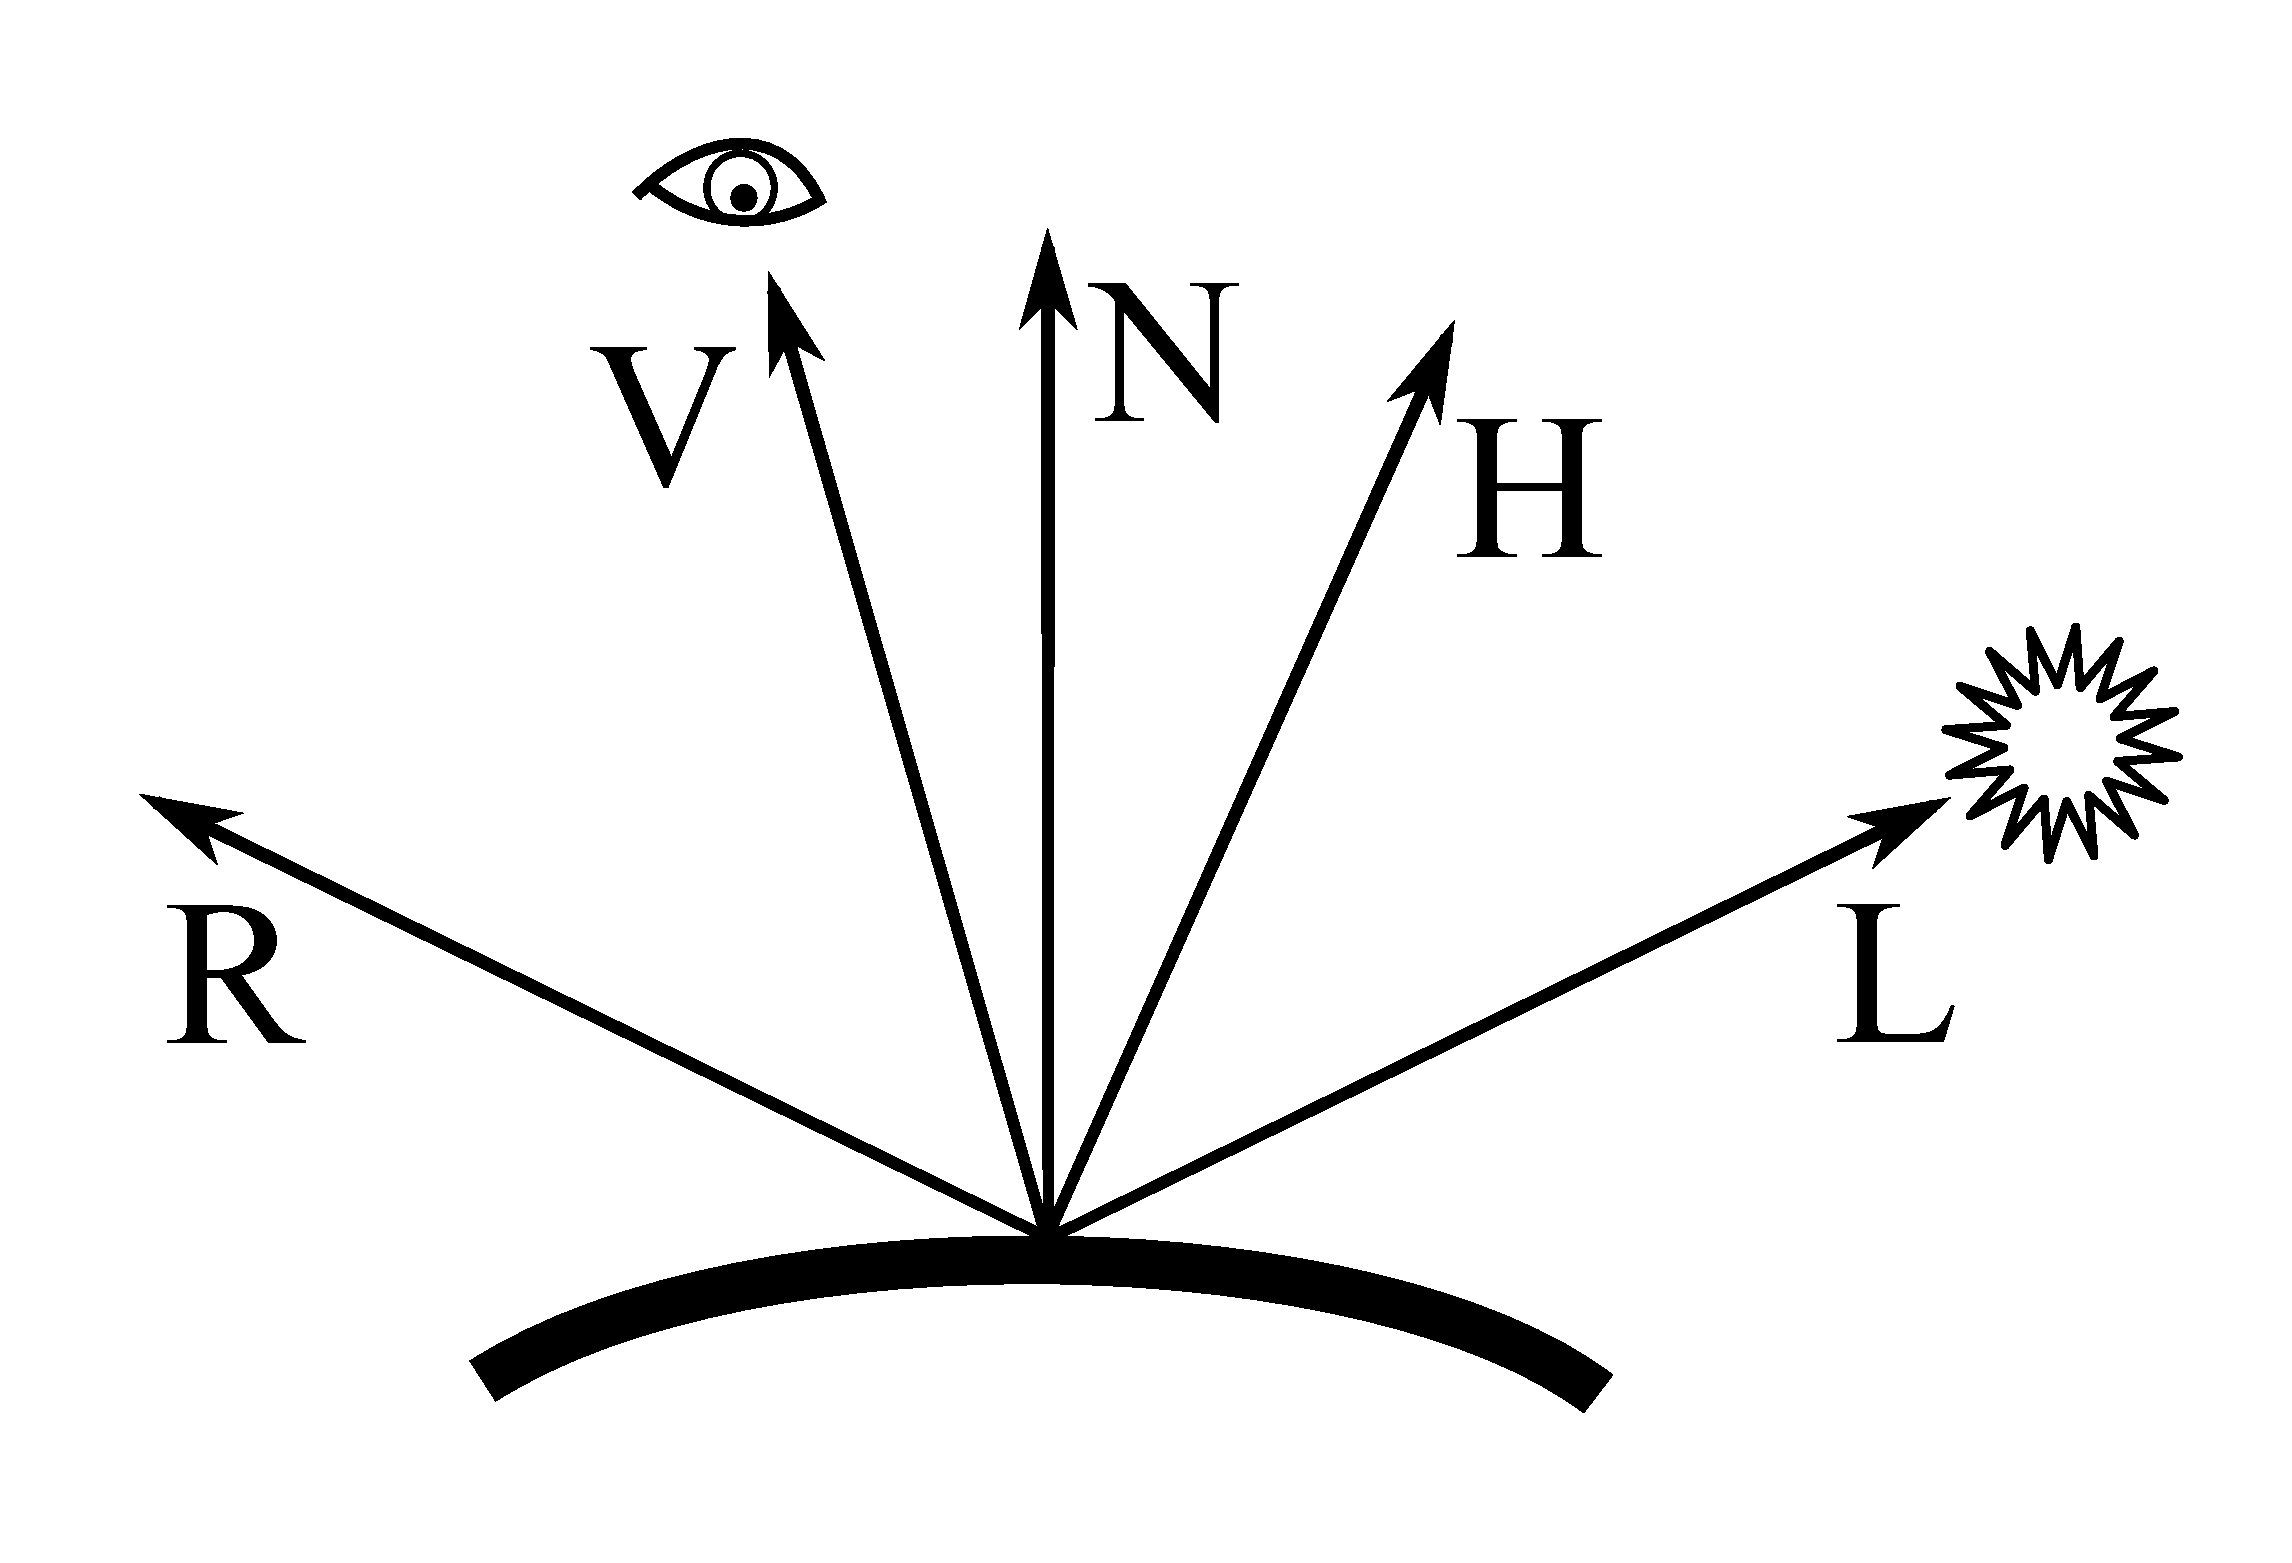
\includegraphics[width=\textwidth]{brdf}
	\caption[Bidirectional Reflectance Distribution Function]{Bidirectional Reflectance Distribution Function $f$\protect\footnotemark}
\end{figure}

\footnotetext{Quelle: http://commons.wikimedia.org/wiki/File:Blinn\_Vectors.svg}
\clearpage

\subsection{Cook-Torrance Modell}

Das Reflexionsverhalten von Oberflächen wird in der Realität wesentlich von der Oberflächenbeschaffenheit des Materials aber auch dem Material an sich bestimmt. Ein realistisches Reflexionsmodell muss diese Oberflächenbeschaffenheiten und das Material berücksichtigen. Je mehr Oberflächenparameter in das Beleuchtungsmodell einfließen können, desto realistischer und plausibler das Ergebnis.

Beispielsweise spiegeln polierte Oberflächen die Umgebung und erhalten Glanzlichter bei direkter Beleuchtung. Irreguläre rauhe Oberflächen streuen das einfallende Licht ungleichmäßig in alle Richtungen. Wachs oder Haut lässt das Licht zum Teil in das Material eindringen und zerstreut es. Die glänzenden Reflexionen von metallischen Oberflächen werden durch die Leitfähigkeit des Materials bestimmt (siehe \fref{sec:pbr-dielektisch}).

Viele Material- und Oberflächenparameter sind im Offline-Verfahren, und besonders in Echtzeitverfahren, nicht simulierbar. In Echtzeitverfahren ist es beispielsweise nicht praktikabel die mikroskopischen Unebenheiten, genannt \textit{Mikrofacetten} oder \textit{Microfecets} (siehe \fref{fig:microfacet}), exakt zu berechenen. Entsprechend wurden einige approximierende Microfacet Modelle entwickelt, die die Interaktion des Lichts mit den Facetten, realistisch abbilden können.

\begin{figure}
	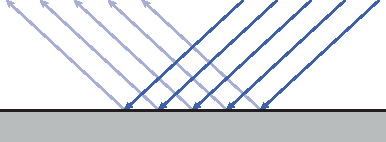
\includegraphics[width=.5\textwidth]{roughness0}
	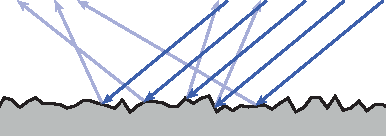
\includegraphics[width=.5\textwidth]{roughness1}
	\caption[Rauheit]{links: $m = 0$; rechts $m = 1$}\label{fig:microfacet}
\end{figure}

Eines von ihnen ist das Cook-Torrance Modell \parencite{Cook1981}, welches mit dem Ziel entwickelt wurde die physikalischen Reflexionseigenschaften von rauhen und glatten Oberflächen realistischer abzubilden, als die klassischen Modelle es ermöglichen \parencite[Seite 40]{Ngan2004}. Da sich das Cook-Torrance Modell auf spekulare Reflexionen konzentriert, verwenden wir das Cook-Torrance Modell auschließlich zur Berechnung des spekularen Anteils $f_s$ der BRDF. Der diffuse Anteil $f_d$ wird durch das klassische Lambert'sche Modell abgebildet und nicht weiter betrachtet. Denkbar sind aber auch andere Modelle für die diffuse Reflexion. In \fref{eq:cook-torrance-model} wird das Modell formal dargestellt
.
\begin{align}
	\label{eq:cook-torrance-model}
	% \caption{Cook-Torrance Illumination}
	f_s(\vV,\vL) = \frac{\mathcal{F}(\vV,\vL)D(\vV,\vL)G(\vV,\vL)}{4(\vN \cdot \vV)(\vN \cdot \vL)}
\end{align}

Der spekulare Beitrag $f_s$ wird durch die drei Faktoren bestimmt: Dem Fresnel $\mathcal{F}$ Term, der Mikrofacetten Richtungsverteilung (Microfacet Distribution Function), $D$ und der geometrischen Abschwächung (Geometrical Attenuation) $G$. Die Auswahl der konkreten Approximationen folgt der aus \cite[Seite 3]{Karis2013}.

\subsubsection[Fresnel]{Fresnel $\mathcal{F}$}
Der Fresnel Effekt beschreibt die Beobachtung, dass Oberflächen stärker reflektieren, umso flacher der Betrachtungswinkel wird. Als Approximation wurde die \textit{Schlick Approximation} \parencite{Schlick1994} gewählt. In \cite{Lagarde2012} wurde eine weitere Modifikation vorgeschlagen, um den Berechnungsaufwand im Shader zu reduzieren. Diese findet hier ebenso ihre Anwendung und wird für unsere Implementierung übernommen. $F_0$ beschreibt die Reflektanz (als Farbwert) für parallel zur Normale $\vN$ einfallendes Licht.

\begin{align}
	\label{eq:fresnel-schlick}
	\mathcal F(\vV,\vL) = F_0  + (1 - F_0) 2^{(-5.55473 (\vV \cdot \vH) - 6.98316 (\vV \cdot \vH))}
\end{align}


\subsubsection[Mikrofacetten Normalverteilung]{Mikrofacetten Normalverteilung $D$} 
Die Funktion $D$ beschreibt die statistische Normalverteilung der Ausrichtung der Mikrofacetten entsprechend der Winkelhalbierenden $\vH$. Die Mikrofacetten von glatten Oberflächen sind überwiegend gleich ausgerichtet, so dass Licht hauptsächlich entlang $R$ reflektiert wird. Raue Oberflächen besitzen eher zufällig ausgerichtete Mikrofacetten, so dass das reflektierte Licht breiter gestreut wird. Die Rauheit der Oberfläche wird mit $m$ im Intervall $[0,1]$ ausgedrückt. Zur Approximation von $D$ finden sich wiederum eine Vielzahl von Modellen. Die Implementierung verwendet das als \textit{GGX} in \cite{Walter2007} vorgestellte Modell (siehe \fref{eq:ggx}).

\begin{align}
	\label{eq:ggx}
	D(\vV,\vL) = \frac{m^4}{ \pi \left(\left( \vN \cdot \vH \right)^2\left(m^4 - 1\right) + 1\right)^2}
\end{align}


\subsubsection[Geometrische Abschwächung]{Geometrische Abschwächung $G$} 
$G$ beschreibt einen Faktor, der die Tatsache simuliert dass Mikrofacetten sich gegenseitig einfallendes oder reflektiertes Licht blockieren und sich somit gegenseitig schattieren ($G_1(\vL)$) oder Reflexionen maskieren ($G_1(\vV)$) können. Verwendet wird eine modifizierte Version der \textit{Schlick} Approximation, damit sie sich dem physikalisch präziseren Smith Modell annähert. Eine genauere Analyse des Smith Modells findet sich in \cite[Kapitel 6, Seite 33]{Heitz2014}.

\begin{align}
	\label{eq:geometric-schlick}
	k &= \frac{(m + 1)^2}{8}\\
	G_1(\vV) &= \frac{\vN \cdot \vV}{(\vN \cdot \vV)(1-k)+k}\\
	G_1(\vL) &= \frac{\vN \cdot \vL}{(\vN \cdot \vL)(1-k)+k}\\
	G(\vV,\vL) &= G_1(\vV) G_1(\vL)
\end{align}


\subsubsection{Dielektische und metallische Materialien}\label{sec:pbr-dielektisch}

\begin{figure}
	
\includegraphics[width=.5\textwidth]{dielectric}
	\includegraphics[width=.5\textwidth]{metallic}
	\caption[Dielektische und metallische Materialien]{links: Plastik; rechts: Messing}
	\label{fig:dielectric-metallic}
\end{figure}

In der Natur lassen sich Substanzen bezüglich ihrer Leiteigenschaften in drei Kategorien einteilen: Nichtleiter (Dielektrikum oder Isolatoren), Halbleiter und Leiter (u.A. metallische Substanzen). Ohne auf die physikalischen Details einzugehen (Details in \cite[Abschnitt: Glanz und Farbe der Metalle]{Zawischa2011}) unterscheiden sich metallische und dielektrische Materialien in ihrem spekularem Reflexionsverhalten. Dielektrische Materialien besitzen ausschließlich weiße spekulare Reflexionen\footnote{unter weißem Licht} während metallische Materialien über ein Farbspektrum spekular reflektieren \parencite[Abschnitt: Specular]{Lagarde2011a}(siehe \fref{fig:dielectric-metallic}).

In der Implementierung wird dies über eine Justierung des $F_0$ Wertes aus dem Fresnel-Term $\mathcal{F}$ abgebildet. Für metallische Materialien wird $F_0$ auf die Grundfarbe (Albedo) des Materials gesetzt und die Grundfarbe auf schwarz, ansonsten wird $F_0$ auf weiß gesetzt (Die Idee basiert auf der \textit{Unreal Engine 4} Implementierung, Stand 2015).

\section{Praktische Umsetzung}
\label{sec:pbr-umsetzung}

Wie Eingangs erwähnt erfordert die Umstellung auf \ac{PBR} eine Anpassung in der Produktion und der Render"-pipeline. Während Diffuse- bzw. Albeo-Texturen sowie Normalentexturen bereits üblich sind, ist es für die Albedo Texturen wichtig, dass sie von jeglicher vorberechneter Beleuchtung bereinigt sind, damit die grundlegenden Texturen in allen Beleuchtungssituationen anwendbar sind (Details in \cite{Lagarde2011}). Die Implementierung der \ac{PBR} Pipeline wird im \fref{sec:src-pipeline} aufgelistet. Im Folgenden eine kurze Übersicht über die praktischen Grundlagen der Implementierung.

\subsection{Eingangsparameter}

\begin{figure}
\centering
	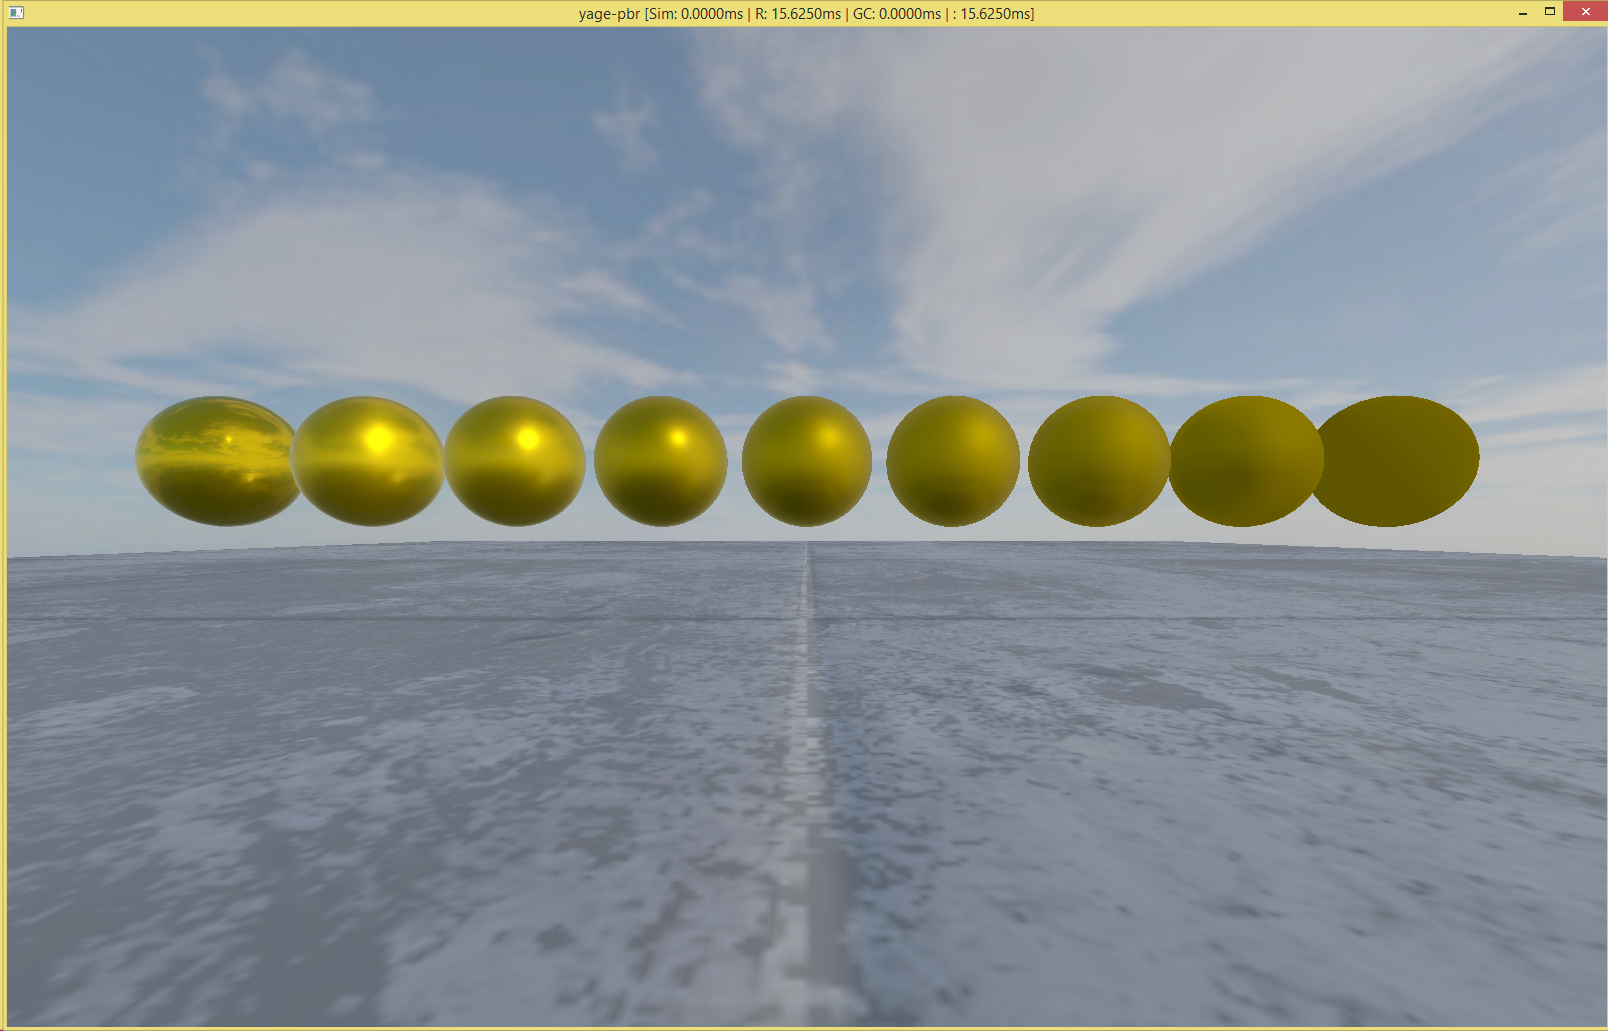
\includegraphics[width=\textwidth]{shots/pbr02}
	\caption{Von links nach recht ansteigender Rauheitswert}
	\label{fig:pbr-roughness}
\end{figure}

Als Eingangsparameter verwendet die Pipeline der Implementierung dieser Arbeit folgende Größen:
\begin{itemize}
\item Albedo-Textur im sRGB Farbraum (\fref{fig:pbr-albedo-tex})
\item Normalen-Textur mit Oberflächennormale im Tangenten-Raum kodiert in RGB (\fref{fig:pbr-normale-tex})
\item Roughness-Textur ($m$) in Graustufen (\fref{fig:pbr-roughness-tex})
\item Metallic-Textur in Graustufen für die Unterscheidung von dielektrischen und metallischen Oberflächen (\fref{fig:pbr-metalmask-tex})\footnote{Entspricht einer Maske, 0 = nicht metallisch, 1 = metallisch}
\end{itemize}

\begin{figure}
\centering
\begin{subfigure}{0.24\textwidth}
	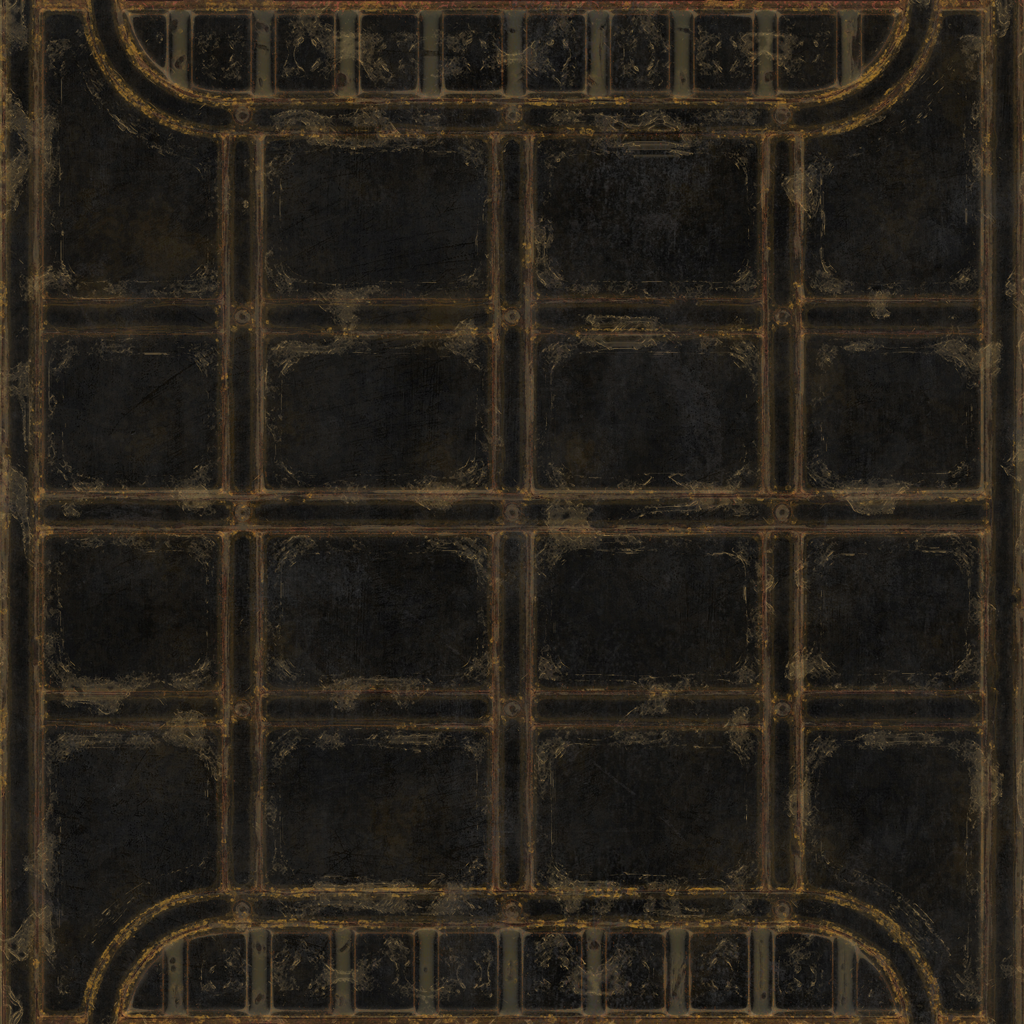
\includegraphics[width=\textwidth]{Door_IronDungeonDoor_1k_alb}
	\caption{Albedo-Textur}\label{fig:pbr-albedo-tex}
\end{subfigure}
\begin{subfigure}{0.24\textwidth}
	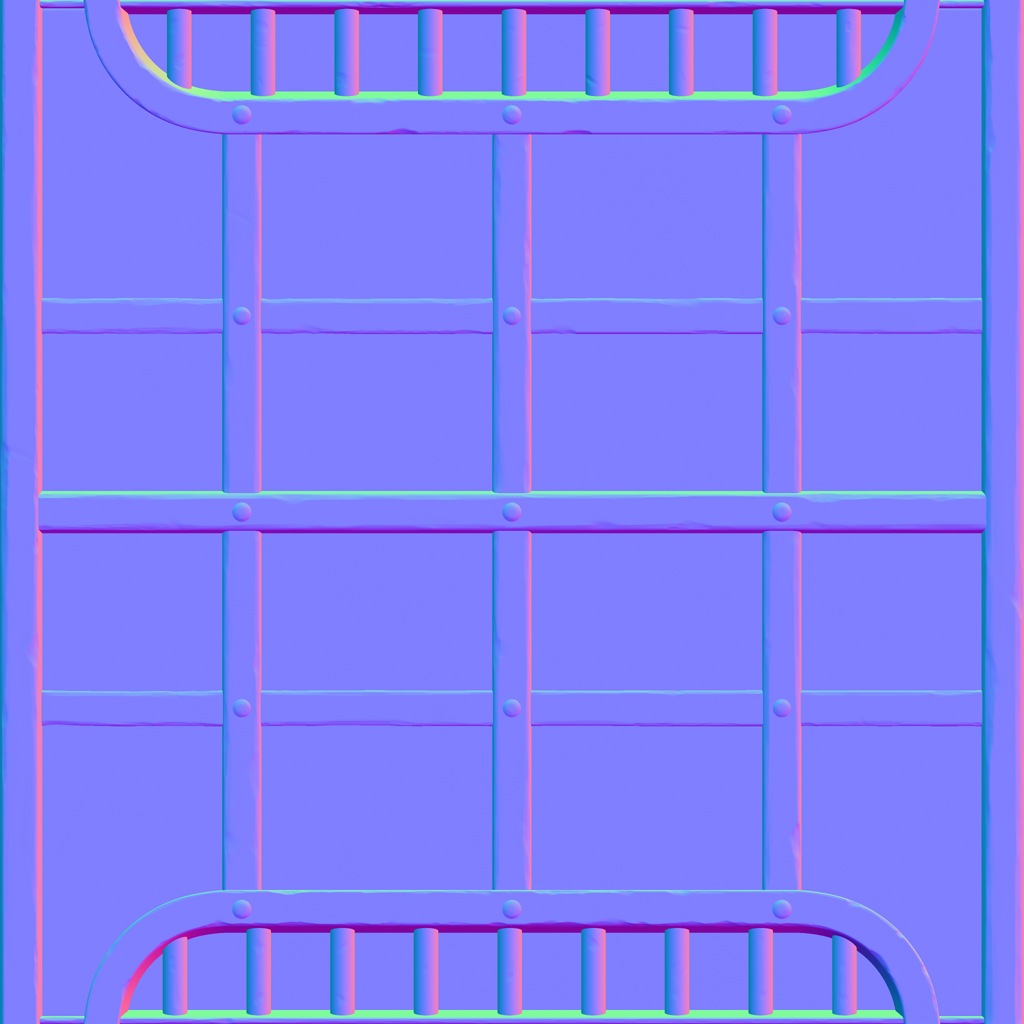
\includegraphics[width=\textwidth]{Door_IronDungeonDoor_1k_n}
	\caption{Normalen-Textur}\label{fig:pbr-normale-tex}
\end{subfigure}
\begin{subfigure}{0.24\textwidth}
	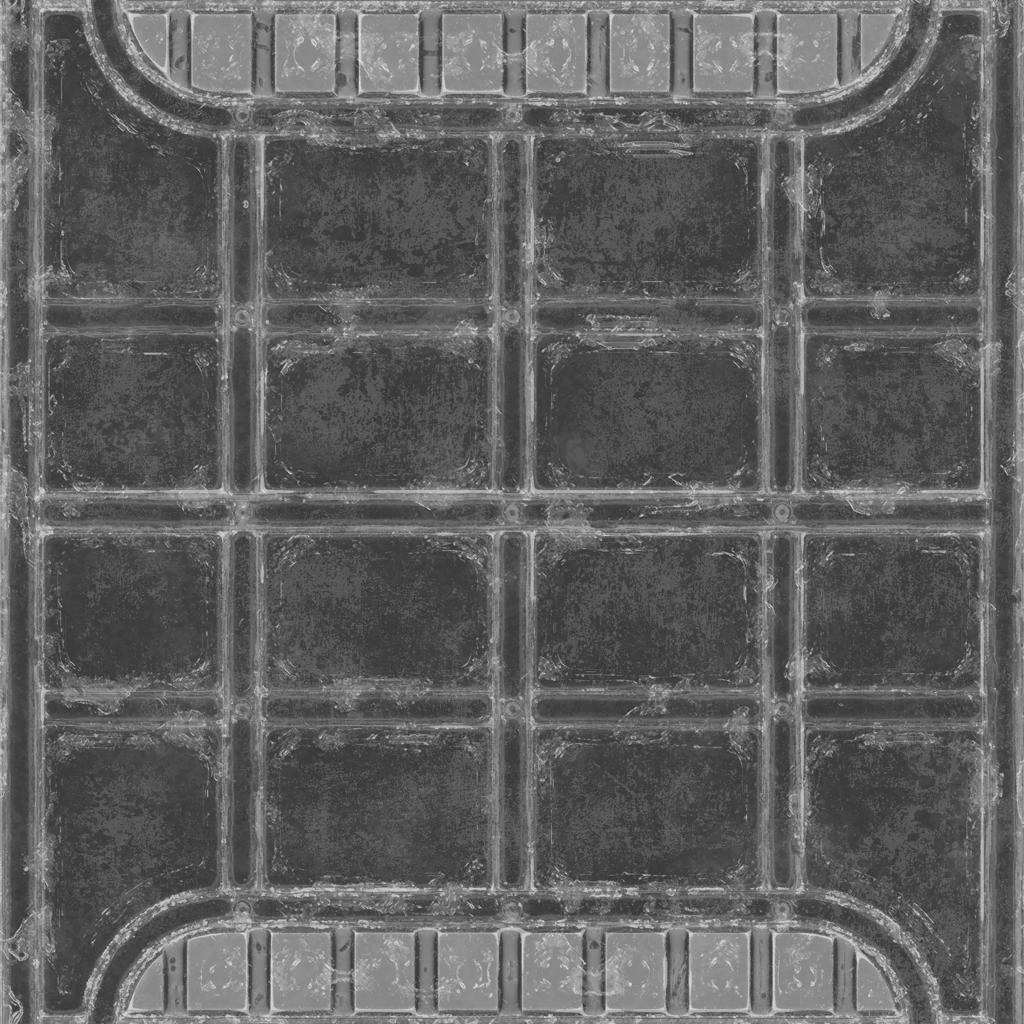
\includegraphics[width=\textwidth]{Door_IronDungeonDoor_1k_g}
	\caption{Roughness-Textur}\label{fig:pbr-roughness-tex}
\end{subfigure}
\begin{subfigure}{0.24\textwidth}
	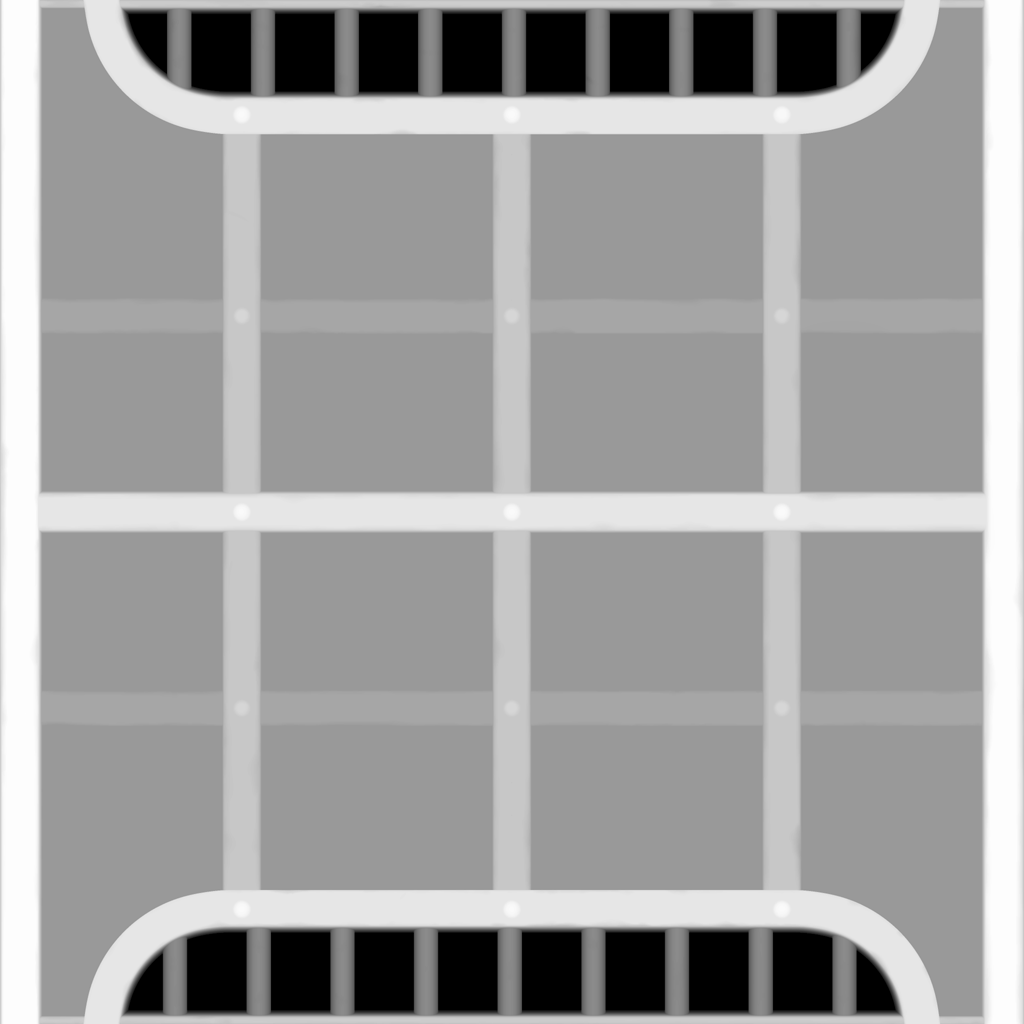
\includegraphics[width=\textwidth]{Door_IronDungeonDoor_1k_h}
	\caption{Metal-Mask-Textur}\label{fig:pbr-metalmask-tex}
\end{subfigure}
\caption{Beispiel eines Textur-Sets}
\label{fig:pbr-texturen}
\end{figure}


\subsection{Renderverfahren}

Als Renderverfahren wurde das als \textit{Deferred Shading} bekannte Verfahren gewählt, da es effizienter als \textit{Forward Shading} in der Lichtberechnung mit vielen Lichtern ist. Dazu wird vor der Berechnung der Schattierung der Oberflächen die Geometrie gerendert. In diesem Renderschritt werden die Oberflächenattribute wie Albedo-Farbe, Roughness und Normale in Texturen gerendert, kombiniert oft \textit{G-Buffer} genannt. Dieser \textit{G-Buffer} dient anschließend im Shading Renderschritt als Grundlage für die Berechnung. In diesem Schritt werden die Lichter mit Stellvertreter Geometrien gerendert. Für jedes so erzeugte Fragment wird die gewählte \ac{BRDF} mit Hilfe der Lichtparameter und der Parameter aus dem G-Buffer ausgewertet. In der fortlaufenden Pipeline werden die Farbwerte im HDR-Raum behandelt. Im abschließenden Tone-Mapping Schritt werden die Farbwerte vom HDR-Raum auf den linearen (s)RGB Raum übertragen. Weiterführende Details finden dazu finden sich in der Implementierung zu dieser Arbeit oder in \cite{Shishkovtsov2005}.

\subsection[Indirekte Beleuchtung]{Indirekte Beleuchtung mit \acl{IBL}}\label{sec:pbr-ibl}

Bisher wurde nur die direkte Beleuchtung von Materialien betrachtet. Aber ein weiterer wesentlicher Beitrag zum realistischen Eindruck ist die sogenannte indirekte Beleuchtung. Indirekte Beleuchtung beschreibt die physikalische Tatsache, dass Objekte nicht nur direkt von Lichtquellen beleuchtet werden, sondern selbst wieder Licht reflektieren. Entweder trifft das reflektierte Licht in das Auge des Betrachters, so dass Objekte für uns sichtbar werden, oder wiederum auf andere Objekte. Letzteres führt dazu, dass Oberflächen, durch das von anderen Oberflächen reflektierte Licht, zusätzlich beleuchtet werden \warn{Bild}. Diese wechselseitige Interreflexion wird unter dem Begriff indirekte Beleuchtung zusammengefasst.

Bisher haben wir in \fref{eq:brdf-dekonstruiert} ausschließlich die \ac{BRDF} mit direkter Beleuchtung betrachtet, aber die \ac{BRDF} lässt sich wie in \ref{eq:brdf-indirect-dekonstruiert} um Beiträge aus ambienten bzw. indirekten Beleuchtungstermen erweitern. Da spekulare Reflexionen kein Sonderfall von glatten Oberflächen sind \parencite{Hable2010}, lohnt ein generelles Verfahren zur Berechnung des indirekten Beitrags $f_{indirect}$. 

\begin{align}
	% \caption{Dekonstruierte BRDF}
	\label{eq:brdf-indirect}
	f   &= f_d + f_s\\
	\intertext{Erweiterung von $f_d$ und $f_s$ um ambienten Beitrag:}
	{f_d}^{\prime} &= f_{d_{indirect}} + f_{d_{direct}}\\
	{f_s}^{\prime} &= f_{s_{indirect}} + f_{s_{direct}}\\
	\label{eq:brdf-indirect-dekonstruiert}
	f^{\prime}   &= \underbrace{f_{d_{indirect}} + f_{s_{indirect}}}_{f_{indirect}} + \underbrace{f_{d_{direct}} + f_{s_{direct}}}_{f_{direct}}
\end{align}

Idealerweise lässt sich die Pipeline um ein umfassendes \acf{GI}\footnote{\acl{GI} Synonym für indirekte Beleuchtung.} Verfahren erweitern, das die wechselseitigen Interreflexionen aller Objekte im Raum über ein möglichst breites Frequenzenband\footnote{niedrige Frequenzen = diffuse Reflexion $f_{d_{indirect}}$; hohe Frequenzen = spekulare Reflexion $f_{s_{indirect}}$} hin abdeckt. Doch voll dynamisches \ac{GI} ist in Echtzeit immer noch nicht vollends praktikabl. Verfahren wie \ac{SVOGI} \parencite{Lin2013} erlauben zwar auch spekulare Reflexionen sind aber praktisch nur auf Highend Hardware durchführbar.

Deswegen findet ein vorberechnetes Verfahren Anwendung. Ein weiterer Grund ist, dass die Implementierung einfacher ist. Zum Einsatz kommt ein erweitertes \acf{IBL} Verfahren, dass die Umgebungstexturen im Preprozess für die unterschiedlichen Frequenzen vorintegriert. Die Vorintegration läuft aktuell noch nicht direkt in der Pipeline, sondern wird offline mit dem von Sébastien Lagarde modifiziertem Programm \textit{AMD Cubemapgen} durchgeführt \parencite{Lagarde2012a}. Dazu wird eine HDR-Cubemap in das Programm geladen und mit den passenden Einstellungen gefiltert. Das Resultat ist eine \ac{PMREM} die dann geladen und in der Auswertung der \ac{BRDF} verwendet wird.

\paragraph{Pre-Filtered Mipmapped Radiance Environment Map} Betrachten wir die Reflexion an einem Oberflächenpunkt aus Sicht des Betrachters, so bestimmt sich die Reflexion aus der Streuung des reflektierten Sichtstrahls ($\vR$). Ein perfekter Spiegel reflektiert den Sichtstrahl ohne jegliche Streuung während rauhe Oberflächen den Strahl mit zunehmender Rauheit entsprechend breiter streuen, bis hin zur ausschließlich diffusen Streuung.

Betrachten wir diffuse und spekulare Reflexionen als diffuse und spekulare indirekte Beleuchtung der Umgebung, lässt sich aus \fref{eq:brdf-indirect-dekonstruiert} folgern, dass sich Reflexionen mit dem $f_{indirect}$ Term abbilden lassen. Für die Rauheit der Oberflächen wurde $m$ als Einflussgröße für den spekularen Anteil der \ac{BRDF} eingeführt. Betrachten wir Umgebungstexturen (\textit{Environment Maps}) als Repräsentation des einfallenden Lichts, können wir Umgebungstexturen für die Berechnung des ambienten Terms $f_{indirect}$ verwenden. Entsprechend der Oberflächen Rauheit muss dafür das einfallende Licht über einen Ausschnitt der Hemisphäre aufgesammelt werden. Dies entspricht der Auswertung der \ac{BRDF} über dem entsprechenden Raumwinkel $\Omega$ (siehe \fref{eq:ambient-integral}). Dies führt zu dem in \fref{eq:ambient-integral} aufgeführtem Integral.

\begin{equation}
	\label{eq:ambient-integral}
	R = \int\limits_{\Omega} f(\vV,\vL)(\vN \cdot \vL)Env(\vL)\, \mathrm{d}\omega_{\vL}\\
\end{equation}

mit $Env(\vL)$ = \text{Wert aus Umgebungstextur entlang Richtungsvektor} $\vL$

Für einen perfekt spiegeligen Oberflächenpunkt reduziert sich der Raumwinkel $\Omega$ auf einen Strahl. Mit steigender Rauheit $m$vergrößert sich der Raumwinkel bis hin zur ganzen Hemisphäre. Wird die gesamte Hemisphäre integriert, entspricht das der diffusen indirekten Beleuchtung. 

Die Auswertung für beliebige $m$ ist zur Laufzeit zu aufwändig. Deswegen wird im Vorfeld eine entsprechende Faltung (Auswertung des Integrals inklusive der \ac{BRDF}) für abgestufte Werte von $m$ im Bereich $[0,1]$ auf die Umgebungstextur angewendet. Die gefalteten Umgebungstexturen werden in den Mipmap-Stufen der Umgebungstextur gespeichert. Dies ermöglicht die Berechnung der Werte $f_{s_{indirect}}$ und $f_{d_{indirect}}$ auf Basis der gefilterten Umgebungstextur zur Laufzeit, indem wir den Rauheitswert $m$ auf die entsprechende Mipmap Stufe abbilden und den Radiance Wert $R$ der Umgebungstextur auswerten.

\begin{figure}
\centering
\begin{subfigure}{0.18\textwidth}
	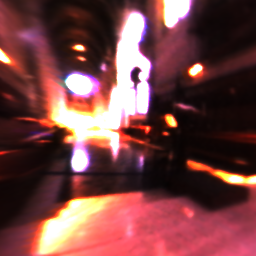
\includegraphics[width=\textwidth]{grace_m00_c00}
	\caption{Basis-Textur}\label{fig:pmrem-basis}
\end{subfigure}
~
\begin{subfigure}{0.18\textwidth}
	
\includegraphics[width=\textwidth]{grace_m01_c00}
	\caption{Stufe 1}\label{fig:pmrem-1}
\end{subfigure}
\begin{subfigure}{0.18\textwidth}
	
\includegraphics[width=\textwidth]{grace_m02_c00}
	\caption{Stufe 2}\label{fig:pmrem-2}
\end{subfigure}
\begin{subfigure}{0.18\textwidth}
	
\includegraphics[width=\textwidth]{grace_m03_c00}
	\caption{Stufe 3}\label{fig:pmrem-3}
\end{subfigure}
\begin{subfigure}{0.18\textwidth}
	
\includegraphics[width=\textwidth]{grace_m04_c00}
	\caption{Stufe 4}\label{fig:pmrem-4}
\end{subfigure}
\caption[Beispiel einer PMREM Textur]{Basis-Textur (\subref{fig:pmrem-basis}) und die ersten vier \ac{PMREM} Stufen einer Fläche der Environment Cubemap (\subref{fig:pmrem-1} - \subref{fig:pmrem-4})}
\end{figure}

\section{Wo wird es eingesetzt?}
\label{sec:pbr-wo}

\ac{PBR} findet inzwischen in folgenden kommerziellen Engines Verwendung:
\begin{itemize}
\item CryEngine (Crysis 3) \parencite{Schulz2014}
\item Unreal Engine 4 \parencite{Martin2012}
\item Frostbite (Battlefield 3 \& 4) \parencite{Lagarde2014}
\item IW-Engine (Call of Duty) \parencite{Lazarov2011}
\item EVE Online Engine \parencite{CCP2014}
\item Killzone: Shadow Fall \parencite{Drobot2013}
\item FOX Engine (Metal Gear Solid) \footnote{http://www.eurogamer.net/articles/digitalfoundry-tech-analysis-mgs5-fox-engine [Abgerufen: \today]}
\end{itemize}


%%%%%%%%%%%%%%%%%%%%%%%%%%%%%% Anwendungsbeispiele
\chapter{Anwendungsbeispiele}
\label{chap:anwendung}

Es folgt eine exemplarische Implementierung eines Tone-Map Render"-schritts. Die Aufgabe des Render"-schritts besteht darin eine HDR-Textur auf einen vom Monitor darstellbaren RGB Farbraum abzubilden. Die eigentliche Abbildung der Farbwerte wird im Shader |"res/glsl/sampling/tonemap.frag"| vorgenommen und ist hier, mit einem Verweis auf die Implementierung, nicht weiter aufgeführt. Die folgende Implementierung wird schrittweise erläutert und in Teilen aus didaktischen Gründen etwas gegenüber der eigentlichen Implementierung vereinfacht. Der zusammenhängende Quellcode dieses Beispiels findet sich in \fref{lst:tonemap-pass-vollstaendig}.

\paragraph{Ressourcenverwaltung} In der Implementierung wird eine eigene |Resource| Monade zur Verwaltung der Ressourcen auf Basis des |resourcet|\footnote{https://hackage.haskell.org/package/resourcet} Pakets verwendet. In dieser |Resource| Monade lassen sich Ressourcen akquirieren (zum Beispiel mit |glResource|) und über die |Applicative| und |Functor| Instanzen kombinieren. Verlässt das Programm den Kontext der |Resource| Monade, zum Beispiel beim Beenden der Renderloop, werden alle Ressourcen über die registrierte Operation freigegeben.

\paragraph{StateVars} StateVars sind eine einfache Kapselung von zwei IO Operationen, von der eine Operation einen Wert abfragt und und die andere Operation einen Wert setzt. Oft werden StateVars in Verbindung mit externen (foreign) Biblitheken verwendet um veränderliche Zustände zu kapseln. StateVars können als normale Haskell Datenobjekte verwendet werden. Eine Ad-Hoc Implementierung findet sich in \fref{lst:statevar}.

\begin{haskell}[label={lst:tonemap-pass-sig},caption={\texttt{ToneMapPass} Signatur},nolol]
type ToneMapInput = (HDRSensor, Texture2D PixelHDR, Maybe (Texture2D PixelHDR))
type ToneMapOutput = (Texture2D PixelRGB8)
type ToneMapPass = RenderPass ResIO ToneMapInput ToneMapOutput
\end{haskell}

Die Eingabe in unser |RenderPass| ist ein Triple aus |HDRSensor|, einer HDR Textur |Texture2D PixelHDR| und einer weiteren optionalen HDR Textur, die additiv mit der ersten gemischt wird. |HDRSensor| ist Teil einer |HDRCamera| und beinhaltet für das Tone-Mapping benötigte Größen, wie den Weiß-Punkt oder die Belichtung (Exposure). Die Ausgabe ist eine übliche RGB Textur.

\begin{haskell}[label={lst:tonemap-pass-res},caption={\texttt{ToneMapPass} Resourcen Allokation},nolol]
toneMap :: Resource ToneMapPass
toneMap = do
  emptyvao <- glResource
  boundVertexArray $= emptyvao
  fbo <- glResource
  
  pipeline <- [ $(embedShaderFile "res/glsl/sampling/drawRectangle.vert")
              , $(embedShaderFile "res/glsl/sampling/tonemap.frag")]
              `compileShaderPipeline` includePaths
  Just (FragmentShader{..}) <- traverse fragmentUniforms =<< get (fragmentShader $ pipeline^.pipelineProgram)

  outTexture <- liftIO . newIORef =<< createTexture2D GL_TEXTURE_2D (Tex2D 1 1) 1

  return $ mkStaticRenderPass $ \(sensor, sceneTex, mBloomTex) -> do
\end{haskell}

In \fref{lst:tonemap-pass-res}, dem Ressourcenblock des Renderschritts, werden die Ressourcen akquiriert, die zur Ausführung der ab \fref{lst:tonemap-pass-run-resize} beschrieben Routine notwenig sind. Dazu gehören ein Vertex Array Objekt, Framebuffer Objekt und die aus dem Vertex-Shader |drawRectangle.vert| und dem Fragment-Shader |tonemap.frag| erzeugte OpenGL Pipeline\footnote{https://www.opengl.org/wiki/GLSL\_Object\#Program\_pipeline\_objects}. Die Uniform Variablen des Fragment-Shaders werden von |fragmentUniforms| als |StateVar|s gekapselt (siehe Verwendung \fref{lst:tonemap-pass-run-pipeline}). Zusätzlich erzeugen wir uns eine interne |IORef| für die Ausgabetextur. Da die verwendeten OpenGL Texturen\footnote{erzeugt mit \texttt{glTexStorage*}} in ihrer Größe unveränderlich sind, muss für neue Ausgabegrößen entsprechend auch jeweils eine neue Textur erzeugt werden (siehe \fref{lst:tonemap-pass-run-reize}). Dieses Texturobjekt speichern wir uns für den nächsten Aufruf in der |IORef|.

\begin{haskell}[label={lst:tonemap-pass-run-resize},caption={[ToneMapPass Größenanpassung des Framebuffers]\texttt{ToneMapPass} Größenanpassung des Framebuffers},nolol]
    target <- get outTexture
    when (target^.textureDimension /= sceneTex^.textureDimension) $ do
      let V2 w h = sceneTex^.asRectangle.extend
      newtarget <- (\t -> resizeTexture2D t w h) =<< get outTexture
      outTexture $= newtarget
      void $ attachFramebuffer fbo [mkAttachment newtarget] Nothing Nothing
    boundFramebuffer RWFramebuffer $= fbo
\end{haskell}

Gegebenenfalls wird die Ausgabetextur in ihrer Größe an die Größe der Basistextur angepasst. Da die Größenanpassung der Textur intern durch das Erzeugen einer neuen Textur durchgeführt wird, muss die neue Textur noch dem Framebuffer neu angefügt werden (\fref{lst:tonemap-pass-run-resize}).

\begin{haskell}[label={lst:tonemap-pass-run-pipeline},caption={\texttt{ToneMapPass} Zuweisung an Uniform Variablen},nolol]
    boundProgramPipeline $= pipeline^.pipelineProgram

    iScene $= sceneTex
    iBloom $= mBloomTex
    iHdrSensor $= sensor
\end{haskell}

In \fref{lst:tonemap-pass-run-pipeline} wird die erzeugte Shaderpipline für diesen Renderschritt aktiviert und den in |StateVar|s gekapselten Uniform Variablen des Fragment-Shaders Werte zugewiesen.

\begin{haskell}[label={lst:tonemap-pass-run-draw-and-out},caption={\texttt{ToneMapPass} Draw-Call und Textur ausgeben},nolol]
    glDrawArrays GL_TRIANGLES 0 3

    get outTexture
\end{haskell}

Abschließend wird der Draw-Call abgesetzt und die nun von OpenGL gefüllte Textur als Ausgabe zurück gegeben (\fref{lst:tonemap-pass-run-draw-and-out}).


%%%%%%%%%%%%%%%%%%%%%%%%%%%%%% Analyse
\chapter{Resultat}
\label{chap:resultat}

In der vorliegenden Arbeit wurde eingangs in \fref{chap:engine-uebersicht} aus den gestiegenen Anforderungen an Softwareprojekte in der Spielebranche die Motivation entwickelt, neue Mittel und Wege für das Beherrschen der zunehmenden Komplexität zu suchen. Es wurde festgestellt, dass die Programmiersprache das wichtigste Kommunikationsmittel unter den Softwareentwicklern ist. Dementsprechend spielt die Programmiersprache eine zentrale Rolle in den Softwareprojekten. Sie bestimmt die Kommunikation aber auch die Softwarearchitektur und die Möglichkeiten der Entwickler.

Jede Branche und jedes Projekt besitzt eigene individuelle Anforderungen und Herausforderungen. In der Grafik-Engine-Entwicklung stellen die Grafik-\ac{API}s die Kernherausforderungen. In \fref{chap:modern-opengl} wurde am Beispiel von \textit{OpenGL} die Entwicklung der Grafik-\ac{API} betrachtet und welche Herausforderungen und Möglichkeiten diese Schnittstelle mit sich bringt.

\fref{chap:loesungen-durch-fp} zitierte Entwicklergrößen aus der Spielebranche. Die getroffenen Aussagen geben die aktuellen Probleme in der Spiele- und Engine-Entwicklung wieder. Es wurde gezeigt, dass die wesentlichen Probleme, die sich in den Industriesprachen C++, C\# oder Java zeigen, in anderen Sprachen entweder konzeptionell keine Probleme darstellen oder bereits gelöst sind. Diese Diskussion wird in diesem Kapitel in \fref{sec:xp-haskell} noch einmal abschließend aufgegriffen und um persönliche Einschätzungen des Autors erweitert.

Aus der Motiviation heraus neue Wege und Lösungen für aktuelle Probleme in der Engine-Entwicklung zu suchen, wurde in \fref{chap:ueberblick-pipeline} eine Renderkomponente einer Engine in Haskell entwickelt. Es wurde gezeigt, dass einfache funktionale Konzepte zu einer hohen Komponierbarkeit der einzelen Bausteine mit geringen Reibungsverlusten führt.

Neben der theoretischen Konzeption war ein wesentlicher Teil dieser Arbeit die praktische Anwendung des Konzepts. Es wurde Eingangs das Ziel gesteckt, dass in \fref{chap:pbr} beschriebene \ac{PBR} Konzept, mit der entwickelten Renderkomponente umzusetzen. Die praktische Umsetzung eines aktuellen Echtzeit-Rendering-Verfahrens dient dabei als praktischer Beweis der Machbarkeit und Anwendbarkeit des Konzepts auf konkrete praktische Problemstellungen. Die Implementierung wird in diesem Kapitel in \fref{sec:diskussion-impl} noch einmal genauer beleuchtet.

\section{Diskussion der Implementierung}\label{sec:diskussion-impl}

Im Fokus deser Arbeit stand die Konzeption der Renderkomponente der Engine, wärhend die Detailbetrachtung der einzelnen Renderschritte in den Hintergrund gerückt ist. Exemplarisch wurde in \fref{chap:anwendung} ein einfacher Renderschritt implementiert, um das generelle Vorgehen zu verdeutlichen. Grundlegende Entscheidungen werden in \fref{sec:konzepte-impl} erläutert und begründet. In \fref{sec:laufzeit-impl} wird das Laufzeitverhalten in der Praxis kurz dargestellt und analysiert.

\subsection{Konzepte der Implementierung}\label{sec:konzepte-impl}

Es wurde für die Implementierung der Renderschritte auf eine Abstraktion der Grafik-\ac{API} verzichtet. Zum einen, da ausschließlich \textit{OpenGL} zum Einsatz kommen sollte, und die Abstraktionsschicht nicht benötigt wurde, um die Grafikschnittstelle flexibel austauschen zu können. Zum anderen sollte die Umsetzung möglichst direkt \textit{OpenGL} verwenden. Dies machte es auch einfacher \textit{OpenGL} Beispiele nach Haskell zu übertragen. Der Verzicht auf eine Abstraktionsschicht reduzierte auch den Aufwand für die Umsetzung des Projekt auf ein vertratbares Niveau. Zudem ist der aktuelle Stand von \textit{OpenGL}\footnote{Version 4.3 zum Zeitpunkt der Projektphase} noch schwer mit funktionalen Konzepten einzufangen (siehe: \fref{chap:haskell-modern-gl}).

Die direkte Umsetzung der Logik eines Renderschritts in \textit{OpenGL} vereinfacht zudem die Verwendung von \textit{OpenGL} Erweiterungen. Dies war für die praktische Umsetzung des \ac{PBR} Verfahrens von Bedeutung, da einige spezielle Erweiterungen\footnote{z.B. ARB\_shading\_language\_include : https://www.opengl.org/registry/specs/ARB/shading\_language\_include.txt} verwendet wurden. Auch in der Implementierung von \acf{AO} mittels \textit{Sparse Textures} wurden spezielle Erweiterungen benötigt.

Anhand von \fref{lst:tonemap-pass-vollstaendig} und \fref{lst:pipeline-vollstaendig} lässt sich erkennen, dass die Trennung und Kapselung der Implementierungsdetails gut funktioniert. Ohne Abstraktionsebene zwischen Anwendung und \textit{OpenGL} ist die Hierarchie der Pipeline-Struktur flach. Später lassen sich gegebenenfalls Abstraktionsschichten einziehen, ohne dass die Pipeline auf der Kompositionsebene angepasst werden muss. Die Struktur der Pipeline auf der Kompositionsebene ist klar und verständlich, die Arrow Notation hilft bei der Zuordnung von Eingaben und Ausgaben. Kleine Renderschritte lassen sich getrennt von einander entwickeln und beispielsweise zu Biblitheken zusammenfassen. Jeder Renderpass kann seine Umgebung und die nötigen Ein- und Ausgaben klar definieren. Konvertierungen von Ein- bzw. Ausgaben können über die vorgestellten Klassen-Instanzen vorgenommen werden.

\subsection{Testszenen}\label{sec:testszenen-impl}

\begin{figure}
\begin{subfigure}{\textwidth}
	\centering
	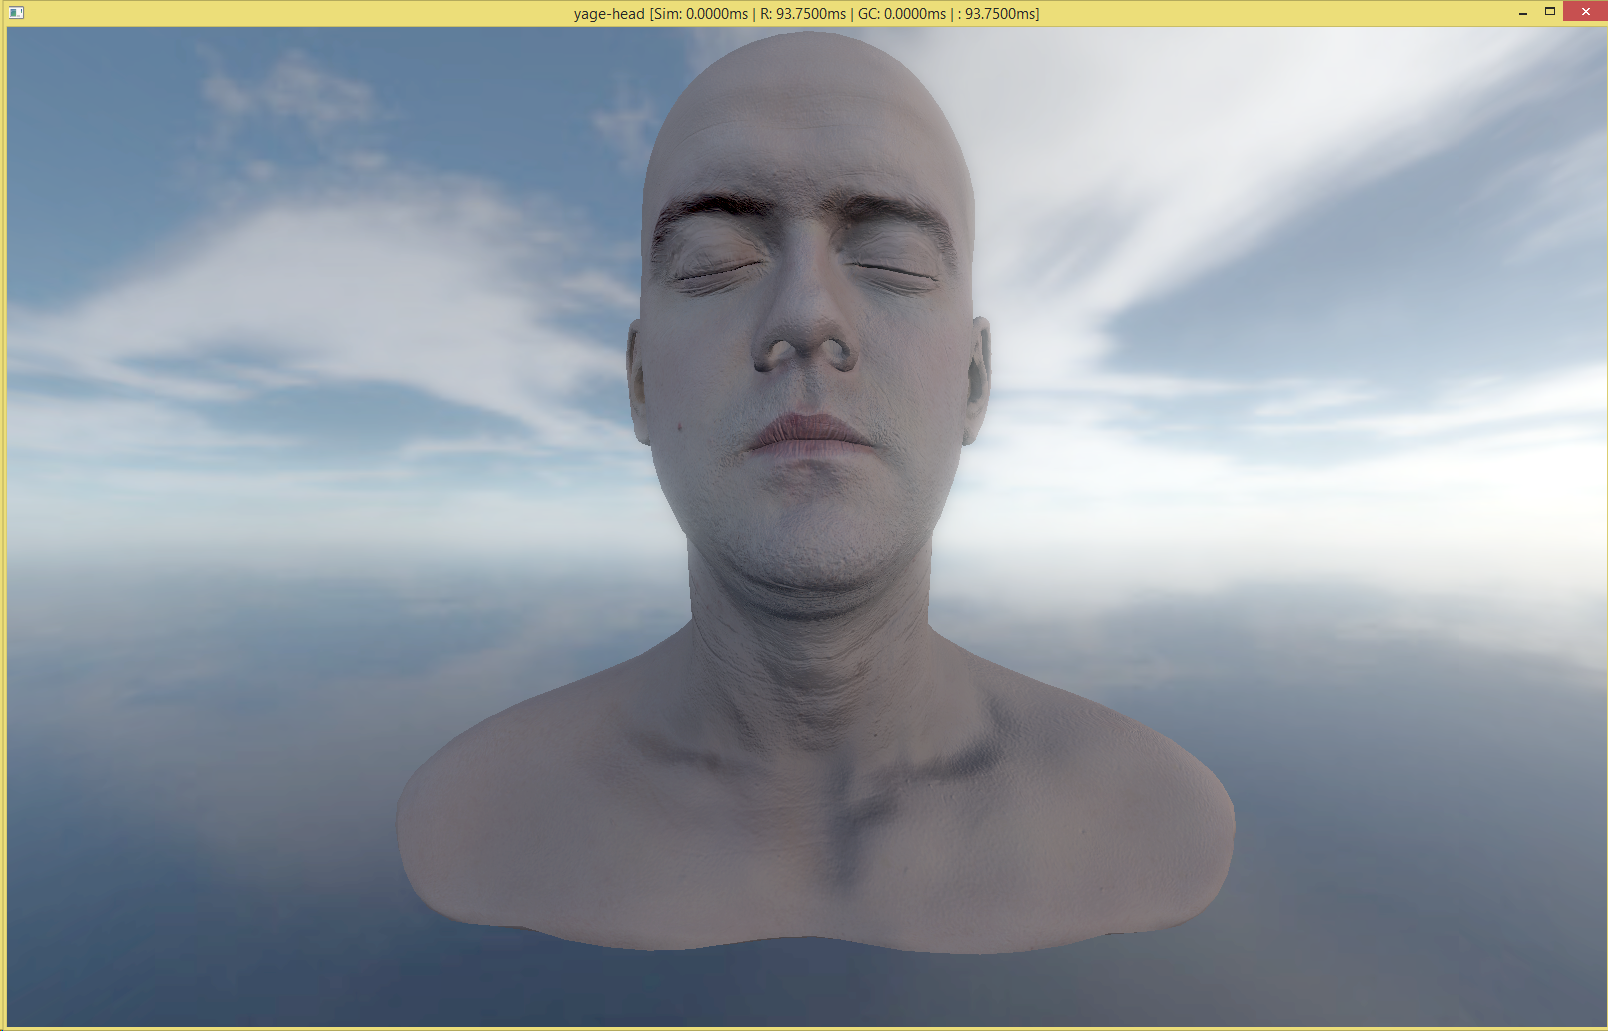
\includegraphics[width=.7\textwidth]{shots/head}
	\caption{Head}\label{fig:impl-scenes-head}
\end{subfigure}\\
\begin{subfigure}{\textwidth}
	\centering
	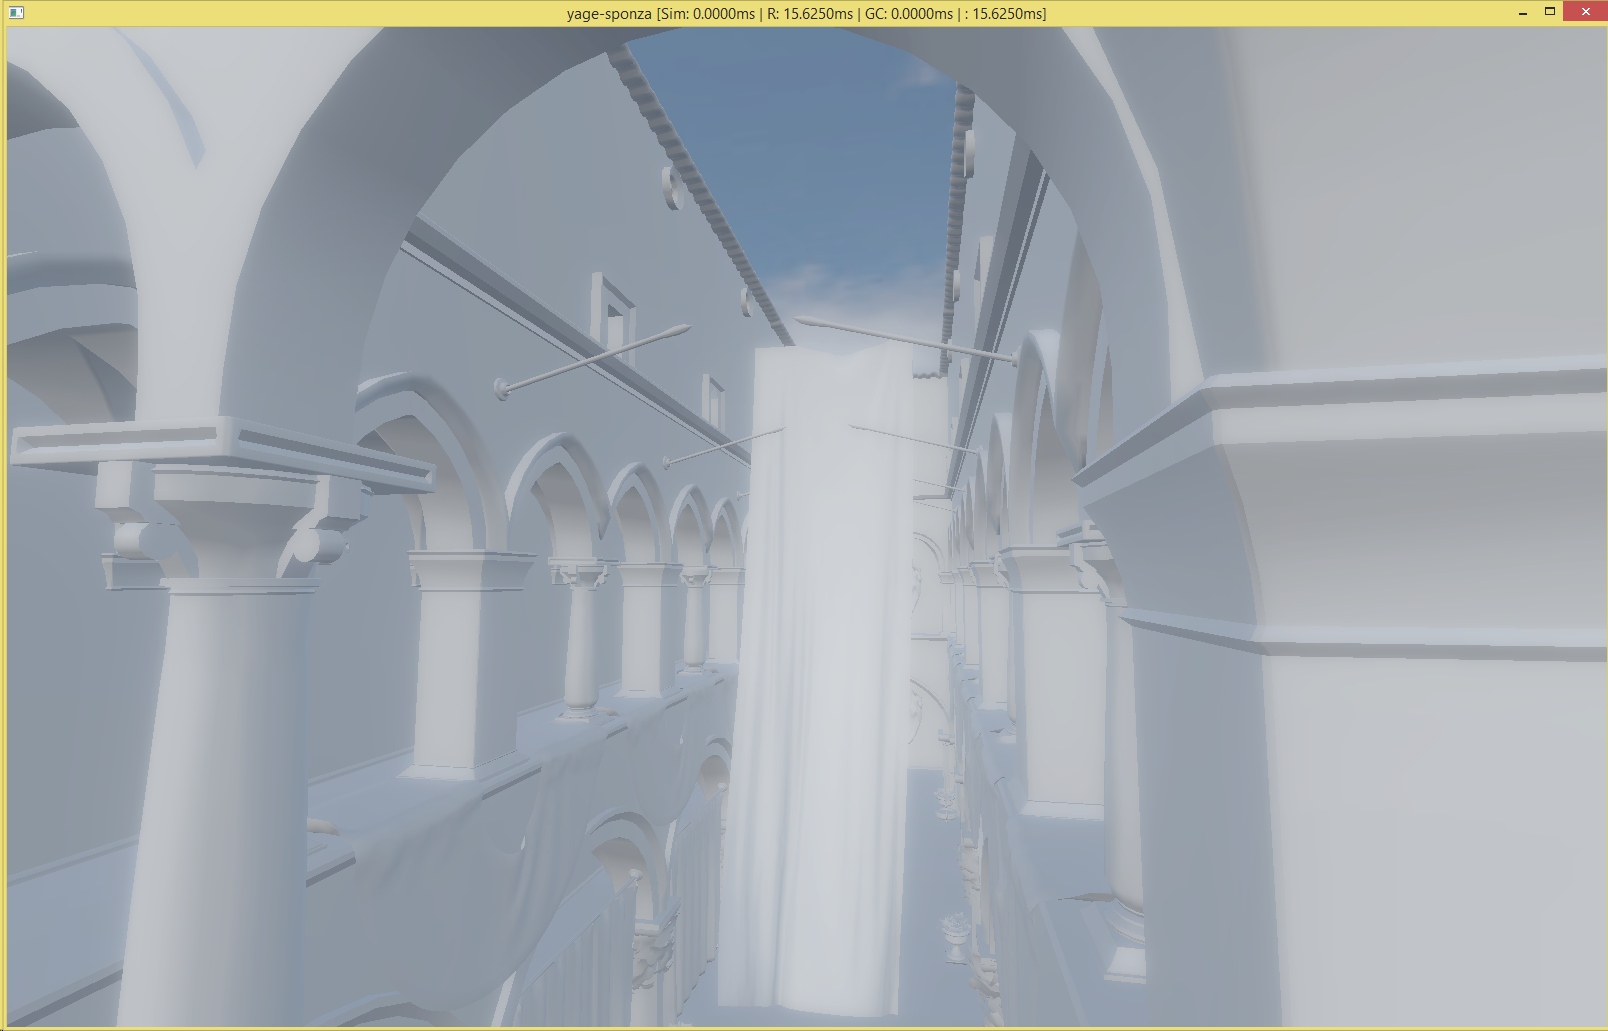
\includegraphics[width=.7\textwidth]{shots/sponza-ibl01}
	\caption{Sponza}\label{fig:impl-scenes-sponza}
\end{subfigure}\\
\begin{subfigure}{\textwidth}
	\centering
	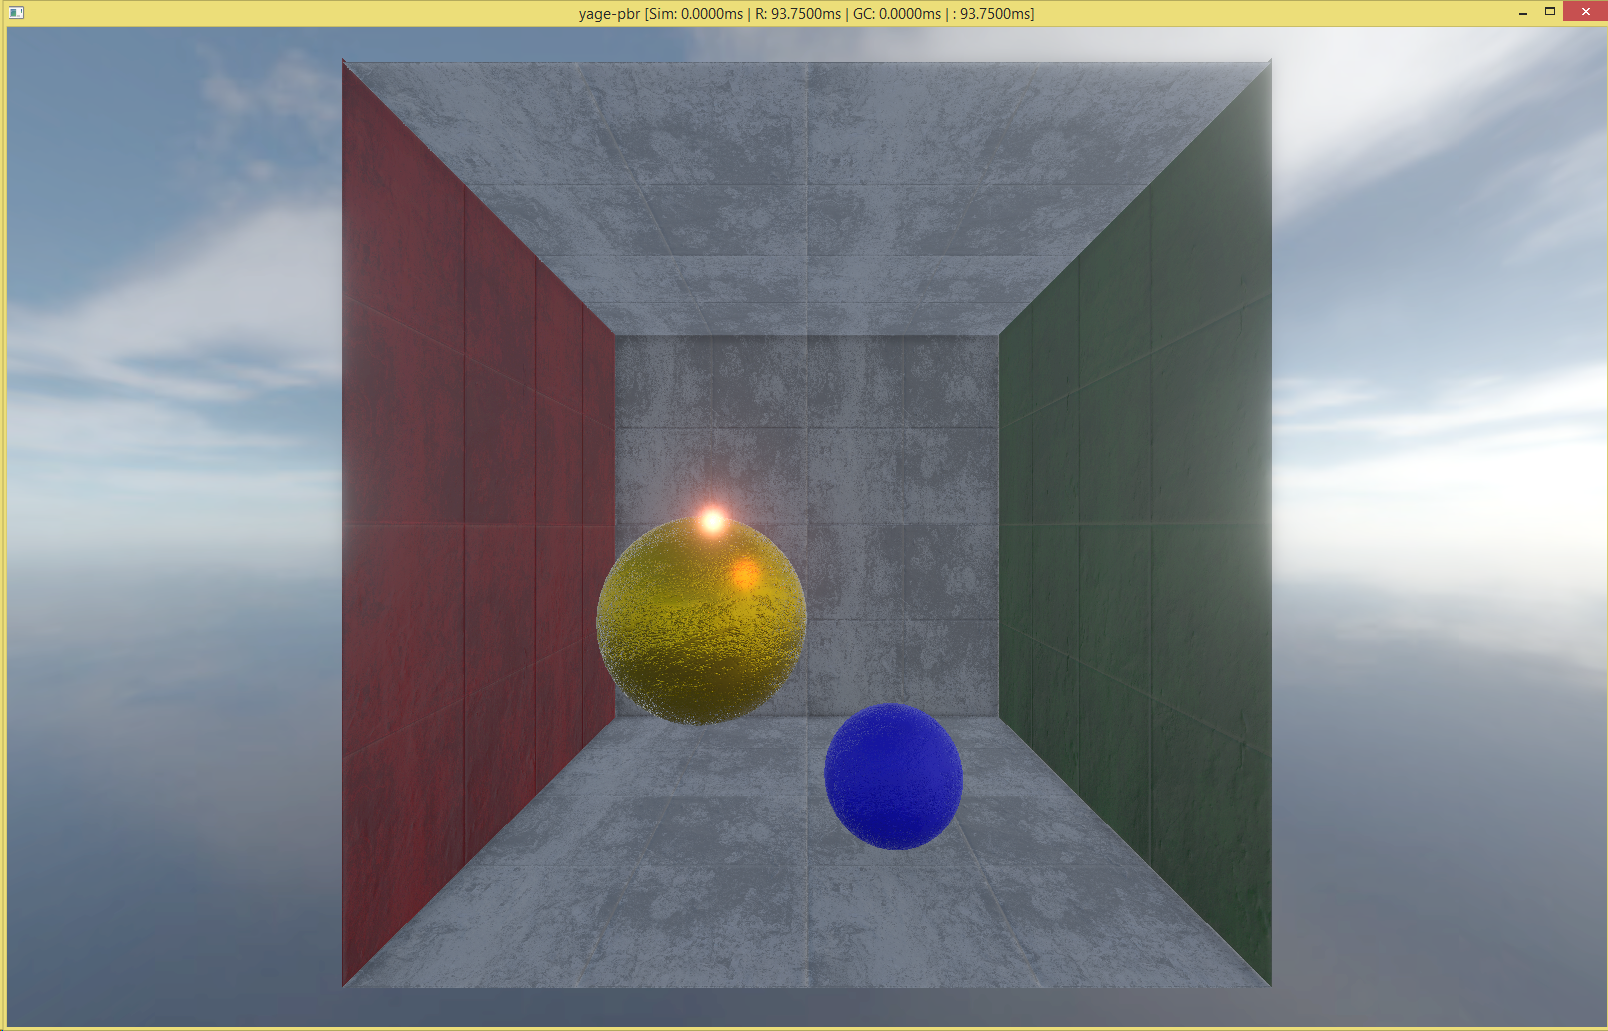
\includegraphics[width=.7\textwidth]{shots/box-blue-start}
	\caption{Box}\label{fig:impl-scenes-box}
\end{subfigure}
\caption{Implementierung Testszenen}\label{fig:impl-scenes}
\end{figure}


Die Testszenen besitzen keinen keinen Anspruch auf Praxisnähe, sondern dienten während der Umsetzung der Engine als Funktionstest. Die Testszene in \fref{fig:impl-scenes-head} diente als Test für das Laden von einem komplexen Modell mit realistischen Texturen. \fref{fig:impl-scenes-sponza} zeigt das Sponza-Modell\footnote{http://www.crytek.com/cryengine/cryengine3/downloads} ohne Texturen aber mit aktiviertem \ac{IBL} auf Basis der gefilterten Umgebungstextur (\fref{sec:pbr-ibl}). \fref{fig:impl-scenes-box} zeigt eine generische Szene mit Testsphären für das Testen der Beleuchtungsparamter der \ac{PBR} Pipeline.

\subsection{Laufzeitverhalten}\label{sec:laufzeit-impl}

Gemessen wurde die durchschnittliche Zeit pro Render-Frame und die prozentuale CPU Last durch das Aufrufen der \textit{OpenGL}-\ac{API}. Drei Szenen (\fref{fig:impl-scenes}) wurden mit dem Programm \textit{nVidia Nsight} ausgewertet. Die Spezifikation des Testsystems ist der \fref{tab:spec-system} zu entnehmen. Die Ergebnisse werden in \fref{tab:performance} dargestellt, jeweils mit und ohne aktiviertem \ac{AO}\footnote{Ambient Occlusion wurde im Zuge des VR Projects implementiert}.


\begin{table}[h]
\centering
\begin{tabular}{@{}lcccc@{}}
\toprule
       & CPU API (\%) & GPU (ms/F) & GPU mit \ac{AO} (ms/F) & \\ \midrule
sponza & 28  		  &  15  & 134  &  \\
head   & 31    		  &  15  & 100  &  \\
box    & 23    		  &  15  & 100  &  \\ \bottomrule
\end{tabular}
\caption{Millisekunden pro Frame für drei Beispielszenen.\\Jeweils ohne und mit Ambient Occlusion}\label{tab:performance}
\end{table}

\begin{table}[h]
\centering
\begin{tabular}{@{}llc@{}}
\toprule
CPU &  Intel(R) Core(TM) i5-3570K CPU \@ 3.40GHz  & \\
GPU &  NVIDIA GeForce GTX 570  & \\
RAM &  32 GB  & \\ \bottomrule
\end{tabular}
\caption{Testsystem}\label{tab:spec-system}
\end{table}

Bisher stand die Performance der Engine nur dann im Fokus, wenn die Performance, trotz der einfachen Szenen, zum Problem wurde. Das war in der Projektphase nur zwei Mal der Fall, aktuell bei der \ac{AO} Implementierung. Techniken zur Reduzierung der API Aufrufe, wie zum Beispiel Frustum-Culling, wurden noch nicht implementiert.

\section{Erfahrungen mit Haskell}\label{sec:xp-haskell}

In der Praxis wird Haskell nicht unvoreingenommen betrachtet. Verfechter von Sprachen wie C/C++ führen das Argument an, Haskell (oder eine andere Sprache) weise eine geringere Laufzeiteffizienz als C/C++ auf. Dies stimmt zwar prinzipiell, doch sind selbst in zeitkritischen Anwendungen nicht alle Komponenten gleich kritisch. Zudem hat die Wahl der geeigneten Algorithmen einen grundlegenderen Einfluss auf die Zeiteffizienz als die Wahl der Programmiersprache. Programmiersprachen sind Kommunikationmittel die an den Menschen gerichtet sind. Entsprechend sollten Programmiersprachen primär als Werkzeug für den Entwickler betrachtet werden, die Form des Problems sollte die Wahl des Werkzeugs bestimmen. In \fref{sec:engines-herausforderungen} und \fref{chap:loesungen-durch-fp} wurden aktuelle treibende Probleme in der Softwareentwicklung benannt und es wurde aufgezeigt, dass Haskell diese Probleme lösen kann oder ihnen gar nicht unterliegt, wie beispielsweise die \texttt{NULL} Problematik oder den \textit{Shared State} in nebenläufigen Anwendungen.

% \begin{figure}
% \centering
% \includegraphics[width=10cm]{benchmarkgame-chart}
% \caption{Benchmark Game: binary-trees\protect\footnotemark}\label{fig:benchmark-chart}
% \end{figure}
% \footnotetext{http://benchmarksgame.alioth.debian.org/u32/performance.php?test=binarytrees}

Die Produktivität der Entwickler sollte nicht unter allen Umständen der Laufzeiteffizient geopfert werden. Ein laufzeiteffizientes und doch gescheitertes Projekt bleibt ein gescheitertes Projekt. Der Gründer von \textit{Epic Games} (\textit{Unreal Engine}) würde 10\% der Performance für 10\% mehr Produktivität opfern \parencite[Seite 20]{Sweeney2006}.


% Next Mainstream Programming Language

\subsection{Vorteile von Haskell}

In \fref{chap:loesungen-durch-fp} wurden schon einige Vorzüge von Haskell diskutiert: Die Möglichkeit zur Abstraktion, die Kompositionsfähigkeit, die Ad-Hoc Beweisführung, das Begünstigen von Multi-Threading durch unveränderliche Daten. Haskell besitzt für viele Probleme in der Softwareentwicklung Lösungen und Lösungskonzepte. 

Abseits der genannten Vorzüge zeigt beispielsweise die Implementierung des Renderschritts in \fref{chap:anwendung}, dass Haskell zudem auch imperative Programmierung erlaubt, sollte dies punktuell notwendig sein. Die Implementierung des Renderschritts folgt in dem Beispiel der imperativen Natur der \textit{OpenGL}-\ac{API}. Hierbei zeigt sich, dass sich funktionale Konzepte gut mit imperativer Programmierung mischen lassen. Viele Konzepte aus Haskell haben inzwischen ihren Einzug in andere imperative Sprachen gefunden: Lambda-Funktionen in C++ und Java, Monaden in C\#\footnote{http://blogs.msdn.com/b/wesdyer/archive/2008/01/11/the-marvels-of-monads.aspx} oder die Strategie Objekte als unveränderlich (immutable) zu entwickeln, damit Multi-Threading sicher und einfacher umgesetzt werden kann \parencite[Seite 46ff]{Peierls:2005:JCP:1076522}.

Ein großer Vorteil von Haskell ist der \ac{GHC}, der eine sehr aktive Entwicklergemeinde besitzt\footnote{https://phabricator.haskell.org/} und fortlaufend verbessert und erweitert wird. Der \ac{GHC} ist ein herausragendes Beispiel für eine "`Real World"' Anwendung von Haskell. Im Vergleich mit dem \textit{gcc} Compiler\footnote{https://gcc.gnu.org/onlinedocs/gcc/Contributors.html} für C/C++ ist die aktive Entwicklergemeine des \ac{GHC} sehr klein\footnote{https://www.haskell.org/ghc/contributors}. C und C++ befinden sich schon jahrelang in einer breiten Anwendung und die Compiler wurden laufend weiterentwickelt und optimiert, teils mit Unterstützung großer Unternehmen wie \textit{IBM} oder \textit{Intel}. Daraus lässt sich schlussfolgern, dass große Fortschritte durch Optimierungen des Compilers nicht mehr zu erwarten sind --- `die "`low hanging fruits"' dürften schon alle gepflückt worden sein'. Haskell und der \ac{GHC} könnten noch einige Optimierungen ermöglichen (Spekulation). Zum einen begünstigt durch die Tatsache, dass viele gereifte Optimierungen aus anderen Sprachen sich nicht ohne weiteres auf Haskell anwenden lassen, und zum anderen eröffnet die Möglichkeit zur Abstraktion in Haskell neue Spielräume für den Compiler. Zum Beispiel erleichtert die referenzielle Transparenz von Haskell dem Compiler sichere Transformationen des Quelltextes\footnote{oder der Zwischensprache} zur Übersetzungszeit vorzunehmen, während in imperativen Sprachen die Neuanordnung von effektbehafteten Operationen nicht trivial ist. Und zum anderen konnten in den \ac{GHC}, aufgrund der kleineren Entwicklergemeinde, in der Summe deutlich weniger Arbeitsstunden investiert werden\footnote{http://www.quora.com/Is-Haskell-as-fast-as-C++-If-not-why-not}.

\subsection{Probleme mit Haskell}\label{sec:probleme-haskell}


Die produktive Verwendung von Haskell bringt aber auch einige Probleme mit sich. Oft sind die Probleme aber eher organisatorischer und menschlicher Natur. Zum einen sind die funktionalen Konzepte, beispielsweise im Vergleich zu den OOP Konzepten, nicht auf breiter Front bekannt und erfordern neue Denkmuster. Die bestehenden Denkmuster konnten sich jahrelang verfestigen. Deswegen stoßen neue Denkansätze auf Widerstand.

Das schrittweise Einführen (Drop In Replacement) von Haskell ist nicht immer einfach. Während sich in modernen Serverarchitekturen selektiv einige kleine isolierte Dienste mit Haskellimplementierungen ersetzen lassen, stellt sich das bei monolithischen Projekten als schwer bis unmöglich heraus. Auch ist die Verknüpfung von Haskell mit C++ noch nicht umfassend gelöst.

Während der Entwicklung auf mehreren Plattformen (Linux, Windows, OS X) traten immer wieder Probleme mit Fremdabhängigkeiten auf. Das Projekt verwendet für \textit{OpenGL} die Bindings aus der Biblithekt |gl|\footnote{http://hackage.haskell.org/package/gl} und zum Erstellen des OpenGL-Kontexts und der Behandlung von Geräteeingaben |GLFW-b|\footnote{http://hackage.haskell.org/package/GLFW-b}. Besonders die Umstellung auf OS X vom \textit{gcc} auf den \textit{Clang}\footnote{http://clang.llvm.org/} Compiler sorgte beim |GHC| für massive Probleme. Projekte mit der |CPP| Direktive konnten zum Teil gar nicht mehr kompiliert werden. Das ist aber kein Alleinstellungsmerkmal von Haskell. Und seit der Einführung der Cabal Sandbox\footnote{http://coldwa.st/e/blog/2013-08-20-Cabal-sandbox.html} können mit Haskell und Cabal mehrere Projekte gleichzeitig und ohne Konflikte oder Abhängigkeitsprobleme entwickelt werden. Zuvor litt das Haskell Ökosystem massiv unter den Abhängigkeitskonflikten, wenn keine isolierten Entwicklungsumgebungen genutzt wurden\footnote{http://www.reddit.com/r/haskell/comments/2al3vx/how\_do\_you\_avoid\_the\_cabal\_hell/}.

Zudem mangelt es Haskell an wirklich umfassenden Entwicklungsumgebungen. Zwar ist die \textit{Emacs} Unterstützung herausragend, doch fehlt es an grafischen \ac{IDE}s, die eine ähnliche Entwicklerunterstützung bieten wie zum Beispiel \textit{Eclipse} für Java oder {Visual Studio} für C++ und .Net. Das schreckt einige Entwickler ab.

Abschließend lässt sich das Fazit zeihen, dass Haskell an Vorurteilen und dem Henne-Ei Problem leidet. Durch die geringe Wahrnehmung von Haskell im produktiven Umfeld wird Haskell die Eignung neben der akademischen Anwendung abgesprochen. Viele kommerzielle Anwendungen von Haskell existieren entweder nur vorborgen oder hinter verschlossenen Türen. Beispielsweise ist es einer Webseite die verwendet Technologie nicht anzumerken\footnote{Chordify verwendet Haskell zur Akkord-Erkennung von Musik: http://chordify.net/}. Ist die Schwelle der Wahrnehmung einmal überschritten, könnten die Vorzüge von Haskell schnell überzeugen. Trotz der geringen Wahrnehmung im praktischen Umfeld, existiert eine Haskell-Gemeinde die regelmäßig Biblitheken entwickelt, die sich aktuellen technologischen Problemen widmen\footnote{reddit.com/r/haskell/}. Sind Entwickler einmal von Haskell überzeugt, scheint Haskell die Motivation zu liefern, weiter in der Sprache zu entwickeln, trotz der geringen Reichweite. Persönlich kann der Autor das bestätigen.


%%%%%%%%%%%%%%%%%%%%%%%%%%%%%% Ausblick
\chapter{Ausblick}
\label{chap:ausblick}

Im Abschluss dieser Arbeit werden noch kurz offene Felder und weitere Ideen für die Zukunft diskutiert.

\paragraph{Material Graph} Auf Basis des entwickelten Rendering-Frameworks könnte in Zukunft eine Bibliothek zur semi-prozeduralen Erzeugung von Materialien entwickelt werden. Die könnte aus Bausteinen bestehen, die sich mittels eines gerichteten Graphens in Abhängigkeit zueinenader setzten lassen. Eine anschließende toplogische Sortierung der Knoten dient zur Auflösung der Abhängigkeiten. Die Bausteine könnten entweder Texturen als Basis in den Graphen importieren oder prozedural erzeugen. Weitere Bausteine filtern, kombinieren oder manipulieren auf sonstigem Wege ihre Eingangskanäle. Die Form der Definition des Rendersystems aus dieser Arbeit weißt schon eine Struktur auf, die das ermöglichen würde. Die Idee stammt aus diversen Material Editoren, wie dem des \textit{Unreal 4 Editors} (siehe \fref{fig:material-graph}) oder \textit{Shader Forge}\footnote{http://www.acegikmo.com/shaderforge/} oder \textit{Substance Designer}\footnote{https://www.allegorithmic.com/products/substance-designer}.

\begin{wrapfigure}{r}{0.4\linewidth}
\centering
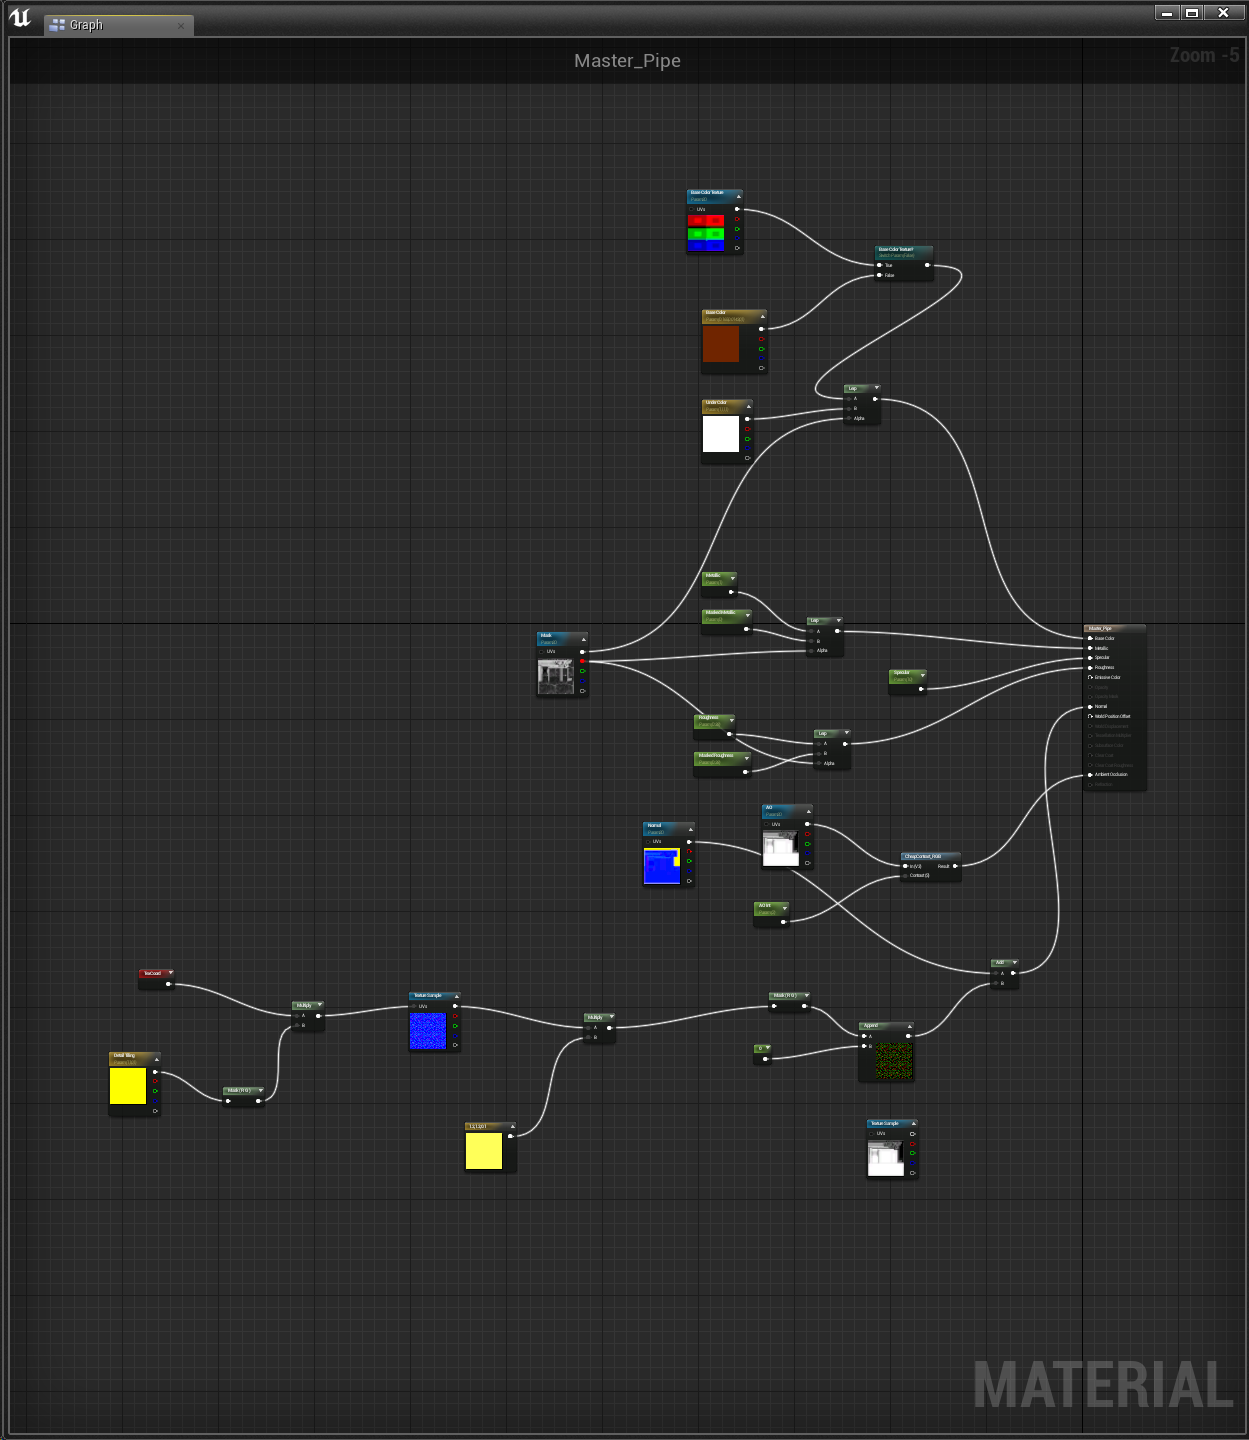
\includegraphics[width=0.4\textwidth]{ue4-material-graph}
\caption{Unreal Engine 4 \mbox{Material Graph}}\label{fig:material-graph}
\end{wrapfigure}

\paragraph{GUI-Framework}\label{sec:gui-framework} Haskell mangelt es an in ausschließlich in Haskell definierten und platformunabhängigen \acsp{GUI}. Bestehende Bindings zu \acs{GUI}-Frameworks sind oft nur unter großem Aufwand, zum Beipsiel unter Windows oder OS X, für einzurichten. Hinzu kommt, dass diese externen Frameworks imperativ gefärbt sind und deswegen oft noch funktional adaptiert werden müssen. Ein ausschließlich auf funktionalen Konzepten (z.B. \ac{FRP}\footnote{http://stud.fh-wedel.de/\~inf9912/research/20131207-info-seminar-frp-netwire/}) basierendes \acs{GUI}-Framework ohne Abhängigkeiten die sich als Hürde für Entwickler und Anwender herausstellen, brächte einige Vorteile für Akzeptanz von Haskell mit sich. Lässt sich erst einmal auf breiter Front produktive Anwendungssoftware entwickeln, die auch nicht nur hinter verschlossenen Türen verwendet wird, dürfte das weitere Aufmerksamkeit von Entwicklern auf Haskell ziehen. Oft wird von außenstehenden Entwicklern berechtigterweise angebracht, dass es wenige "`Real World"' Anwendungen von Haskell gibt oder wenn es sie gibt, sie nur versteckt hinter verschlossenen Türen existieren und nicht bewusst wahrgenommen werden, wie dies zum Beispiel bei Server-Anwendungen der Fall ist.

\paragraph{Vulkan \& SPIR-V} Zu den Kernzielen von \textit{Vulkan} gehören zum einen die Reduzierung des \acs{API}-Overheads und die Reduzierung der \ac{API} auf die modernen und wesentlichen Funktionen (\fref{sec:vulkan}) aber auch zum anderen in der Entwicklung einer expliziten \acs{API}. Sollte dies gelingen, drüfte sich der Umfang der \acs{API} deutlich reduzieren, und so könnten sich neue Möglichkeiten für die funktionale Adaptierung der Grafik-\acs{API} entwickeln. Die explizite \ac{API} könnte es zum ersten mal bei vertretbaren Aufwand ermöglichen die \ac{API} in einer relativ kompakten \ac{DSL} abzubilden. Da sich Haskell selbst sehr gut zur Definition, Parsen und Übersetzen von Sprachen eignet, könnte mit der Zwischensprache \textit{SPIR-V} sich die Möglichkeit auftun, eine (Teil-) Menge von Haskell direkt nach \textit{SPIR-V} hin zu übersetzen. Beispielsweise mittels der \acf{GHC}-\acs{API}, wie dies bei \textit{GHCJS}\footnote{https://github.com/ghcjs/ghcjs} bereits realisiert ist.


%%%%%%%%%%%%%%%%%%%%%%%%%%%%%% Appendix

\appendix

%%%%%%%%%%%%%%%%%%%%%%%%%%%%%% Bib

%%%%%%%%%%%%%%%%%%%%%%%%%%%%%% Bib
\nocite{*}
\printbibliography[heading=head]



%%%%%%%%%%%%%%%%%%%%%%%%%%%%%% Quellen
\chapter{Quellen}

\section[ToneMapPass]{\texttt{ToneMapPass}}
\label{sec:src-tonemappass}

\begin{haskell}[label={lst:tonemap-pass-vollstaendig},caption={\texttt{ToneMapPass} vollständig}]
type ToneMapInput = (HDRSensor, Texture2D PixelHDR, Maybe (Texture2D PixelHDR))
type ToneMapOutput = (Texture2D PixelRGB8)
type ToneMapPass = RenderPass ResIO ToneMapInput ToneMapOutput

toneMap :: Resource ToneMapPass
toneMap = do
  emptyvao <- glResource
  boundVertexArray $= emptyvao

  pipeline <- [ $(embedShaderFile "res/glsl/sampling/drawRectangle.vert")
              , $(embedShaderFile "res/glsl/sampling/tonemap.frag")]
              `compileShaderPipeline` includePaths

  Just (FragmentShader{..}) <- traverse fragmentUniforms =<< get (fragmentShader $ pipeline^.pipelineProgram)

  outTexture <- liftIO . newIORef =<< createTexture2D GL_TEXTURE_2D (Tex2D 1 1) 1
  fbo <- glResource
  return $ mkStaticRenderPass $ \(sensor, sceneTex, mBloomTex) -> do
    target <- get outTexture
    when (target^.textureDimension /= sceneTex^.textureDimension) $ do
      let V2 w h = sceneTex^.asRectangle.extend
      newtarget <- (\t -> resizeTexture2D t w h) =<< get outTexture
      outTexture $= newtarget
      void $ attachFramebuffer fbo [mkAttachment newtarget] Nothing Nothing

    boundFramebuffer RWFramebuffer $= fbo

    glDisable GL_DEPTH_TEST
    glDepthMask GL_FALSE
    glDepthFunc GL_ALWAYS
    glDisable GL_BLEND
    glDisable GL_CULL_FACE
    glFrontFace GL_CCW

    boundVertexArray $= emptyvao
    boundProgramPipeline $= pipeline^.pipelineProgram

    iScene $= sceneTex
    iBloom $= mBloomTex
    iHdrSensor $= sensor
    
    glDrawArrays GL_TRIANGLES 0 3

    get outTexture
\end{haskell}

\section[StateVar]{\texttt{StateVar}}
\label{sec:src-statevar}

\begin{haskell}[label={lst:statevar},caption={Definition \texttt{StateVar}}]
data StateVar a = StateVar (IO a) (a -> IO ())

($=) :: StateVar a -> a -> IO ()
(StateVar _ setter) $= a = setter a

get :: StateVar a -> IO a
get (StateVar getter _) = getter
\end{haskell}

\begin{landscape}
\section{Deferred PBR Pipeline Übersicht}
\label{sec:src-pipeline}
\lstinputlisting[language=Haskell]{src/deferred-pbr-pipeline.hs}
\end{landscape}

\chapter[DVD mit Projektquellen]{DVD mit Projektquellen}\label{chap:dvd}

Quellen auf Github mit Entwicklungsumgebung, Windows Binaries und konsolidierten Quellen:
https://github.com/MaxDaten/yage-meta/releases/tag/0.6.1


\chapter{Eidesstattliche Erklärung}
Ich erkläre hiermit an Eides Statt, dass ich die vorliegende Arbeit selbstständig 
und ohne Benutzung anderer als der angegebenen Hilfsmittel angefertigt 
habe; die aus fremden Quellen direkt oder indirekt übernommenen Gedanken 
sind als solche kenntlich gemacht. 
Die Arbeit wurde bisher in gleicher oder ähnlicher Form keiner anderen Prüfungskommission vorgelegt
und auch nicht veröffentlicht.

\begin{flushright}
Ort, Datum  \ Unterschrift (Vor- und Nachnahme)
\end{flushright}


\thispagestyle{empty}
% \cleardoublepage
\null\newpage



\end{document}
